\cotefile{144}
\scanpage{168}

\[
\sigma_1,\sigma_2,\sigma,\rho_1,\rho_2
\]
\[
\left.
\begin{gathered}
\sigma_1^2=\sigma_2^2=(\sigma_1\sigma_2)^2=1\\
\sigma_1\sigma_2=\sigma^2,\quad
\sigma_1(\sigma)=\sigma_2(\sigma)=\sigma^{-1}
\end{gathered}
\right\}
\begin{array}{l}
D_\sigma\ \text{\unsure{engendré} par }\sigma_1,\sigma_2,\sigma\\[-2pt]
\shortparallel\\[-2pt]D_4
\end{array}
\]
\[
\left.
\begin{gathered}
\sigma_i(\rho_j)=\rho_{\unsure{j}}^{-1}\\
\sigma(\rho_1)=\rho_2
\end{gathered}\right|
\Rightarrow \sigma(\rho_2)=\rho_1
\]
\[
\deleted{\unsure{\sigma}}\qquad
D_\sigma*_{D_{\sigma_1}}D_{\rho_1}
\quad(\text{\unsure{engendré} par }\rho_1,\sigma_1)
\]

\figure{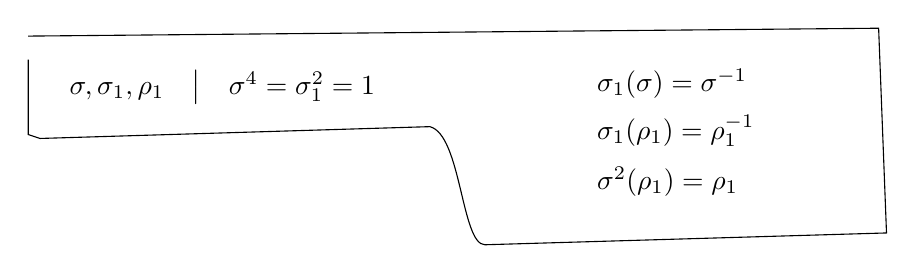
\begin{tikzpicture}[x=1cm,y=1cm]
\draw (0,2)--(10.8,2.1)--(10.9,-.5)--(5.8,-.65)
 .. controls (5.5,-.65) and (5.5,.75) .. (5.1,.85)
 --(.15,.7)--(0,.75)--(0,1.7);
\node[anchor=west] at (.4,1.35) {$\sigma,\sigma_1,\rho_1\quad\big|\quad
 \sigma^4=\sigma_1^2=1$};
\node[anchor=west] at (7.1,1.4) {$\sigma_1(\sigma)=\sigma^{-1}$};
\node[anchor=west] at (7.1,.8) {$\sigma_1(\rho_1)=\rho_1^{-1}$};
\node[anchor=west] at (7.1,.15) {$\sigma^2(\rho_1)=\rho_1$};
\end{tikzpicture}}
\[
\sigma_2=\sigma_1\underset{\text{\unsure{centre}}}{\underbrace{\sigma^2}}\ 
\unsure{\text{et}}\ \text{\unsure{commute à}}\ \sigma_1
\qquad \sigma_1\sigma_2=
\]
\[
\sigma_2(\unsure{\rho_1})=
\]

\figure{\begin{tikzpicture}[x=1cm,y=1cm]
\draw (-3,1.35)--(7.8,1.65);
\node at (-1.3,.15) {$\sigma^2-$};
\draw (1,0) ellipse (1.4 and 1.25);
\draw[->] (1,1.2)--(1,-1.15);
\draw (1.04,1.08)--(.96,-.65);
\draw[->] (2.3,0)--(-.3,.04);
\draw (1.9,-.08)--(.15,.02);
\draw[->] (2.28,-.6) .. controls (2.25,-.95) and (2,-1.13) .. (1.9,-1.15);
\end{tikzpicture}}
\[
\left\{\begin{aligned}
\sigma_1e_1&=e_1\\
\unsure{e_1|\sigma_1}e_2&=-e_2
\end{aligned}\right.
\qquad
\left\{\begin{aligned}
\sigma_2e_1&=-e_1\\
\sigma_2e_2&=e_2
\end{aligned}\right.
\qquad
\left\{\begin{aligned}
\sigma e_1&=e_2\\
\unsure{\sigma}e_2&=-e_1
\end{aligned}\right.
\]

\figure{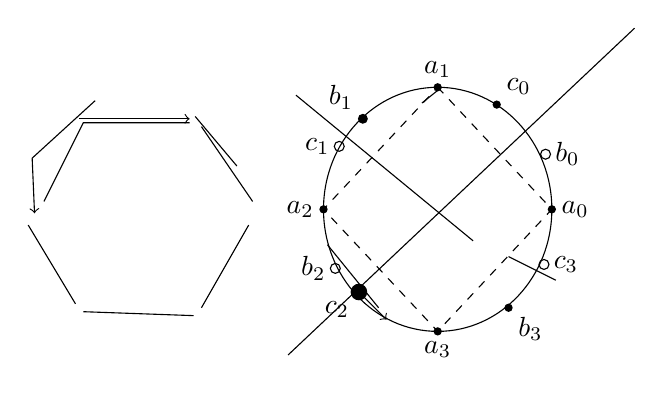
\begin{tikzpicture}[x=1cm,y=1cm]
\draw (-4,.9)--(-3.5,1.9)--(-2.15,1.9);
\draw (-2,1.85)--(-1.35,.9);
\draw (-1.4,.6)--(-2,-.45);
\draw (-2.1,-.55)--(-3.5,-.5);
\draw (-3.6,-.4)--(-4.2,.6);
\draw[->] (-3.55,1.95)--(-2.15,1.95);
\draw[->] (-3.35,2.18)--(-4.15,1.45)--(-4.12,.75);
\draw (-2.08,1.98)--(-1.55,1.35);
\draw (1,0.8) ellipse (1.45 and 1.55);
\draw[dashed] (1,2.35)--(2.45,.8)--(1,-.75)--(-.45,.8)--cycle;
\draw (-.8,2.25)--(1.45,.4);
\draw (-.9,-1.05)--(3.5,3.1);
\draw (.8,2.15)--(1.05,2.35);
\draw (1.9,.2)--(2.5,-.1);
\draw (.25,-.45)--(-.4,.35);
\fill (2.45,.8) circle (1.5pt) node[right] {$a_0$};
\fill (1,2.35) circle (1.5pt) node[above] {$a_1$};
\fill (-.45,.8) circle (1.5pt) node[left] {$a_2$};
\fill (1,-.75) circle (1.5pt) node[below] {$a_3$};
\draw (2.37,1.5) circle (1.8pt) node[right] {$b_0$};
\fill (.05,1.95) circle (1.8pt) node[above left] {$b_1$};
\draw (-.3,.05) circle (1.8pt) node[left] {$b_2$};
\fill (1.9,-.45) circle (1.5pt) node[below right] {$b_3$};
\fill (1.75,2.13) circle (1.5pt) node[above right] {$c_0$};
\draw (-.25,1.6) circle (1.8pt) node[left] {$c_1$};
\fill (0,-.25) circle (3pt) node[below left] {$c_2$};
\draw (2.35,.1) circle (1.8pt) node[right] {$c_3$};
\draw[->] (0,-.25)--(.35,-.6);
\end{tikzpicture}}
\[
\rho_1e_1=e_1\qquad
\rho_1e_2=\deleted{\unsure{e_1}}e_2-e_1
\]
\[
\unsure{\tau'_4|\sigma'_1}=
\begin{pmatrix}1&0\\0&-1\end{pmatrix}
\qquad
\underset{\substack{\shortparallel\\\tau_\infty}}
 {\unsure{\tau''_4|\sigma''_2}}=
\begin{pmatrix}-1&0\\0&1\end{pmatrix}
\qquad
\sigma=\begin{pmatrix}0&-1\\1&0\end{pmatrix}
\]
\figure{\begin{tikzpicture}\draw (0,.1)--(0,0)--(2.1,0)--(2.1,.1);\end{tikzpicture}}
\[
\unsure{\rho_0|\rho_1}=
\begin{pmatrix}1&-1\\0&1\end{pmatrix}
\deleted{\unsure{\rho_1}}
\qquad
\unsure{\sigma_1}\xi_0=\rho'\xi'_0=\xi_1
\]
\margin{168}
\scanpage{169}

UNIVERSITE DES SCIENCES

ET TECHNIQUES DU LANGUEDOC

M A T H E M A T I Q U E S \hfill 21.10.80

\begin{center}
SEMINAIRE D'ALGEBRE

1980-1981
\end{center}

Vendredi de 10 h à 12 h, Salle 431 du Bâtiment de Mathématiques.

31 Octobre, J. HELMSTETTER (Institut Fourier, Université de Grenoble I)

\uline{Algèbres de Clifford et groupes de Clifford.}

\uline{Une sous-variété remarquable $XE$ dans l'algèbre extérieure $\unsure{A|\Lambda}E$.}

Soit $E$ un espace vectoriel de dimension finie sur le corps commutatif $K$ ; $XE$ est l'ensemble des éléments de $\Lambda E$ de la forme $x\wedge\operatorname{Exp}u$, où $x$ est un élément décom-\newline
posable de $\Lambda E$ (il est possible que $x\in K$) et où $u\in\Lambda^2E$ ; le symbole $\operatorname{Exp}$ désigne une exponentielle dans la sous-algèbre paire de $\Lambda E$. On commence par le théorème suivant : le produit intérieur d'un élément de $XE$ par un élément de $XE^*$ (où $E^*$ est le dual de $E$), est encore dans $XE$.

Application : soit $Q$ une forme quadratique sur $E$ et soit $B$ une forme bilinéaire (pas nécessairement symétrique) telle que $Q(a)=B(a,a)$ pour tout $a\in E$ ; on peut ``déformer'' le produit extérieur de l'algèbre $\Lambda E$ pour en faire un nouveau produit (noté $xy$) isomorphe à celui de l'algèbre de Clifford associée à $Q$ ; ainsi l'espace vectoriel $\Lambda E$ devient une algèbre $\Lambda(E,B)$ isomorphe au quotient de l'algèbre tenso-\newline
rielle $TE$ par l'idéal bilatère engendré par les éléments $a\unsure{\otimes}\unsure{a-}Q(a)$ ; si $x$ et $y\in XE$, on démontre que $xy\in XE$.

\uline{Indications sur les exposés suivants} : On étudie l'algèbre $\Lambda(E,B)$ mentionnée ci-dessus

Il existe une application involutive $x\to x'$ de $XE$ dans lui-même telle que $xx'=x'x\in K$ et $xax'\in E$ quels que soient $x\in XE$ et $a\in E$. Le groupe de Clifford $X(E,B)$ est l'ensemble des éléments de $XE$ inversibles dans $\Lambda(E,B)$ ; on définit un homomorphisme surjectif de $X(E,B)$ sur le groupe orthogonal $GO(E,Q)$ (groupe des automorphismes de $E$ qui conservent $Q$ ainsi que tous les éléments de $E$ orthogonaux à $E$).

\hfill A. MICALI

\uline{N.B.} Le Séminaire d'Algèbre se fera, cette année, à une cadence d'un exposé par mois sur \uline{les Algèbres de Clifford et Groupes de Clifford} et de trois à quatre exposés par mois sur les \uline{Automorphismes des anneaux de polynômes et séries formelles}.

\margin{169}
\scanpage{170}
\diagram{\begin{tikzcd}
(z,s)\arrow[r] & (\varepsilon z\exp 2\pi as,\ \varepsilon's)
\end{tikzcd}}
\margin{$\varepsilon,\varepsilon'\in\mu$\par $a\in\unsure{\mathbb Q|\mathbf Q}$}

\figure{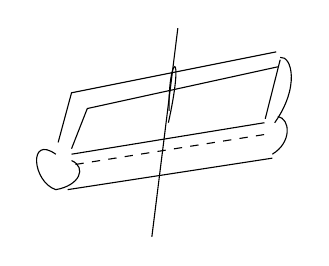
\begin{tikzpicture}[x=1cm,y=1cm]
\draw (0,.25) .. controls (-.35,.5) and (-.3,-.1) .. (0,-.2)
 .. controls (.3,-.15) and (.4,.08) .. (.2,.17);
\draw (.15,-.2)--(2.75,.2);
\draw (.2,.25)--(2.65,.65);
\draw[dashed] (.25,.12)--(2.65,.5);
\draw (.03,.4)--(.2,1.03)--(2.8,1.55);
\draw (.2,.32)--(.4,.83)--(2.82,1.36);
\draw (2.75,.25) .. controls (3,.4) and (2.98,.7) .. (2.82,.73);
\draw (2.78,.65)..controls (3.1,1.1) and (3,1.5)..(2.85,1.48);
\draw (2.66,.7)--(2.85,1.45);
\draw (1.22,-.8)--(1.55,1.85);
\draw (1.43,.65)..controls (1.65,1.65) and (1.42,1.5)..(1.44,.8);
\end{tikzpicture}}
\[
(z\exp 2i\pi as)^{(-1)^\nu},\quad\varepsilon s
\]
\[
\deleted{\varepsilon\ \varepsilon'}\qquad D_\infty\times\mu
\]
\figure{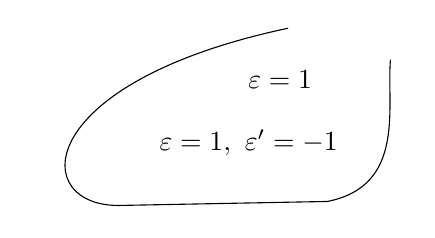
\begin{tikzpicture}
\draw (2.3,1.8)..controls (-1,1.1) and (-1,-.5)..(.2,-.45)
 --(2.8,-.4)..controls (3.8,-.2) and (3.55,.8)..(3.6,1.4);
\node at (2.2,1.15) {$\varepsilon=1$};
\node at (1.8,.35) {$\varepsilon=1,\ \varepsilon'=-1$};
\end{tikzpicture}}

\figure{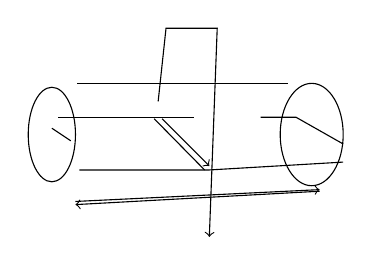
\begin{tikzpicture}[x=1cm,y=1cm]
\draw (0,0) ellipse (.3 and .6);
\draw (3.3,0) ellipse (.4 and .65);
\draw (.32,.65)--(3,.65);
\draw (.35,-.45)--(2,-.45)--(3.7,-.35);
\draw (.08,.22)--(1.8,.22);
\draw (2.65,.22)--(3.1,.22)--(3.7,-.12);
\draw (0,.08)--(.24,-.08);
\draw[->] (1.35,.42)--(1.45,1.35)--(2.1,1.35)--(2,-1.3);
\draw[->] (1.4,.2)--(2,-.4);
\draw (1.3,.2)--(1.94,-.45);
\draw[->] (.3,-.85)--(3.4,-.7);
\draw[->] (3.4,-.72)--(.3,-.89);
\end{tikzpicture}}
\[
\sigma_1(z,s)=(z^{-1},s)\qquad
\underline a(z,s)=(-z,-s)
\]
\[
\sigma_2(z,s)=(z,\deleted{\unsure{-}}s)
\]
\[
\deleted{\unsure{\rho}}\Theta(z,s)=(z\exp 2i\pi s,s)
\]
\figure{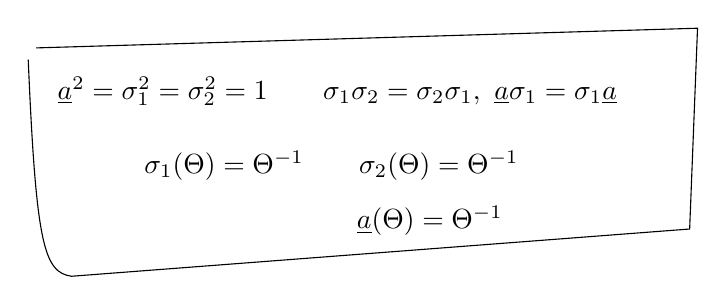
\begin{tikzpicture}[x=1cm,y=1cm]
\draw (0,2.1)--(8.4,2.35)--(8.3,-.2)--(.45,-.8)
 .. controls (.1,-.75) and (0,-.4)..(-.1,1.95);
\node[anchor=west] at (.15,1.55)
 {$\underline a^2=\sigma_1^2=\sigma_2^2=1\qquad
 \sigma_1\sigma_2=\sigma_2\sigma_1,\ 
 \underline a\sigma_1=\sigma_1\underline a$};
\node[anchor=west] at (1.25,.6)
 {$\sigma_1(\Theta)=\Theta^{-1}\qquad\sigma_2(\Theta)=\Theta^{-1}$};
\node at (5,-.1) {$\underline a(\Theta)=\Theta^{-1}$};
\end{tikzpicture}}
\margin{\[
\begin{gathered}
(z^{-1}\exp 2i\pi s,s)\\
(z\exp -2i\pi s,s)\unsure{)}\\
z\exp -2i\pi s,+s\\
-z\exp -2i\pi s,-s\\
z\exp -2i\pi s,s)
\end{gathered}
\]}
\[
\underline a\quad\alpha,\beta,\Theta
\]
\margin{170}
\scanpage{171}

U N I V E R S I T E

DES SCIENCES ET TECHNIQUES

DU LANGUEDOC

\verb|^^^^^^^^^^^^|

\hfill Montpellier, le 14 octobre 1980

Service de la Scolarité

MA/gs

Diffusion : Liste A

N° 5254

\begin{center}
\uline{AVIS DE SOUTENANCE D'UNE THESE DE DOCTEUR-INGENIEUR}

``\uline{AGRONOMIE OPTION ZOOTECHNIE}''
\end{center}

\uline{NOM et prénom du candidat} : DELAVEAU Alain

\uline{Titre de la thèse} : ``CONTRIBUTION A L'ETUDE DE LA MORTALITE DES LAPEREAUX ENTRE LA NAISSANCE ET LE SEVRAGE - (Aspects\unsure{.} physio-\newline
logiques et zootechniques).''

\uline{Date, heure et lieu de soutenance prévus} : 17 octobre 1980 à 9 heures,30

Ecole Nationale Supérieure Agronomique

\uline{Nom du directeur de thèse} : M. L. DAUZIER

\uline{Désignation du laboratoire où la thèse est préparée} : Laboratoire de Physiologie animale à l'E.N.S.A. de Montpellier

\uline{Analyse de l'ouvrage} : La mortalité des lapereaux entre la naissance et le sevrage n'apparaît pas comme un phénomène aléatoire puisque l'essentiel des pertes seproduit durant la première semaine après la mise bas. On note d'ailleurs des causes identiques de pertes de lapereaux dans des élevages expérimentaux différents.

La qualité du nid joue, de plus, un rôle essentiel. C'est ainsi qu'il est possible de diminuer la mortalité post-natale en aménageant le nid le jour, ou même, 10 jours après la parturition. De plus, nous avons enregistré moins de pertes en utilisant des boîtes à nid équipées d'un fond creux. Mais, nous n'avons pas noté d'effet de la température interne de cette même boîte à nid sur les pertes de lapereaux.

Enfin, nous n'avons pas mis en évidence d'incidence de la séparation mère-lapereaux sur la mortalité entre la naissance et le sevrage.

\uline{Durée approximative des recherches ayant abouti à la thèse} : 4 ans

\uline{Composition du jury proposé} :
\begin{tabular}{l}
M. L. DAUZIER\\
M. JD. BAYLE\\
M. M. PRUD'HON\\
M. F. LEBAS\\
M. Y. REYNES
\end{tabular}

\begin{flushright}
P/ Le Secrétaire Général\\
L'Attachée d'administration\\
Universitaire,

\unsure{Gentil}

\uline{A. GENTIL}
\end{flushright}
\margin{171}
\scanpage{173}

\diagram{\begin{tikzcd}
\underset{a}{\bullet}\arrow[r,"\ell"]\arrow[dr,bend right=18,"\ell'"']&
\gamma^{-1}(a)\\
&\gamma'^{-1}(a)
\end{tikzcd}}
\[
(\gamma,\ell)(\gamma',\ell')=(\gamma\gamma',\gamma'^{-1}(\ell)\circ\ell')
\]
\[
(\gamma.\ell)(\gamma'.\ell')=(\gamma\gamma')
 \underbrace{\gamma'^{-1}\ell\gamma'}\,\ell'
\]
\diagram{\begin{tikzcd}[column sep=large]
\underset{a}{\bullet}\arrow[rr,Rightarrow]\arrow[dr,no head,"\ell'"']&&
(\gamma\gamma')^{-1}a=\gamma'^{-1}(\gamma^{-1}a)\\
&\gamma'^{-1}(a)\arrow[ur,"\gamma'^{-1}(\ell)"']&
\end{tikzcd}}

\[
\widetilde u\widetilde v\widetilde u^{-1}\widetilde v^{-1}
\]
\diagram{\begin{tikzcd}
\gamma a\arrow[r,"\ell"]&\underset{a}{\bullet}\arrow[r]&\gamma^{-1}a\\
\gamma'a\arrow[ur,bend right=15,"\ell'"']&&
\end{tikzcd}}
\[
(\gamma,\ell)(\gamma',\ell')
=(\gamma\gamma',\deleted{\unsure{\gamma'(\ell)\circ\ell'}}
 \inserted{\ell\circ\gamma(\ell')})
\]
\diagram{\begin{tikzcd}
&\gamma(a)\arrow[dr,"\ell"]&\\
\gamma\gamma'a\arrow[ur,no head,"\gamma(\ell')"]
 \arrow[dr,"\deleted{\unsure{\gamma'(\ell)}}"']&&\underset{a}{\bullet}\\
&\gamma'(a)\arrow[ur,"\ell'"]&
\end{tikzcd}}
\diagram{\begin{tikzcd}
1\arrow[r]&\Pi\arrow[r,no head]&E\arrow[r,no head]&G\arrow[r,no head]&1
\end{tikzcd}}
\[
(\ell,\gamma)(\ell',\gamma')=(\ell.\gamma(\ell')
\]
\[
\boxed{(\ell,\gamma)(\ell',\gamma')=(\ell\unsure{,|.}\gamma(\ell'),\gamma\gamma')}
\]
\margin{$\gamma.\ell$}

\[
\alpha=u\underline a^{-1}\varepsilon_3(\tau')
\qquad
\beta=u\underline b^{-1}
\]
\diagram{\begin{tikzcd}
\unsure{u}\arrow[r,mapsto]&
\deleted{\unsure{u_a}\quad a=\varepsilon_3(\tau')\alpha^{-1}u,\quad b=\beta^{-1}u}
\end{tikzcd}}
\[
\begin{aligned}
\widetilde{\unsure{\eta}}
 &=\deleted{\unsure{\beta(}}\widetilde\beta
     \widetilde\sigma(\widetilde\beta)^{-1}
 & &=\unsure{\eta}_0\zeta(6\nu)\\
\widetilde\sigma(\widetilde{\unsure{\eta}})
 &=\widetilde\sigma(\widetilde\beta)\widetilde\beta^{-1}
   =\widetilde{\unsure{\eta}}^{-1}
 & &=\widetilde\sigma(\unsure{\eta}_0)\zeta(6\nu)
   =\unsure{\eta}_0^{-1}\zeta(6\nu)
\end{aligned}
\]
$\widetilde\sigma^2$ \unsure{ne commute à} $\widetilde\beta$ que si
$\deleted{\unsure{\beta}}\unsure{\nu_2}=0$
i.e. $\nu=2\nu'$.

\figure{\begin{tikzpicture}\draw (0,0)..controls (1,-.1) and (3,.3)..(4,.4);\end{tikzpicture}}

\[
\widetilde{\unsure{\eta}}=\unsure{\eta}_0=[\beta_0,\sigma_0]
=\beta_0(\sigma_0)\sigma_0^{-1}
=\underline u(\sigma_0)\sigma_0^{-1}
\]
\[
\widetilde\sigma=\sigma_0\zeta(3)
\]
\[
\deleted{\widetilde{\unsure{\eta}}=u(\widetilde\sigma)\widetilde\sigma^{-1}=u(}
\]
\[
\widetilde{\unsure{\eta}}
=\underline u(\widetilde\sigma)\widetilde\sigma^{-1}
=\underline u(\sigma_0)\zeta(3\mu)\sigma_0^{-1}\zeta(-3)
=\underline u(\sigma_0)\sigma_0^{-1}
  \zeta\bigl(\underbrace{3(\mu-1)}_{6\nu}\bigr)
\]
\[
\begin{array}{ccc}
\beta(\widetilde\sigma)&=&u(\widetilde\sigma)\\
\shortparallel&&\shortparallel\\
\beta(\sigma_0)\zeta(3)&&\unsure{u}
\end{array}
\]
\margin{173}
\scanpage{174}

UNIVERSITE DES SCIENCES

ET TECHNIQUES DU LANGUEDOC

M A T H E M A T I Q U E S \hfill 30.10.80

\begin{center}
SEMINAIRE DE GEOMETRIE DIFFERENTIELLE

Mardi 4 novembre, 9 h, Salle 331

A. MEDINA
\end{center}

``La courbure des métriques invariantes à gauche sur les groupes de Lie'' d'après J. MILNOR.

\[
\widetilde\eta=\eta_0\qquad \widetilde{\unsure{\xi}}=\unsure{\xi}_0
\]
\[
\begin{aligned}
\widetilde u(\widetilde\varepsilon_0)
 &=\widetilde u(\widetilde\sigma\widetilde\rho)
 =\deleted{\unsure{\zeta}}\zeta(\nu')\widetilde\eta\widetilde\sigma
   \zeta(-\nu'')\widetilde{\unsure{\xi}}\widetilde\rho\\
 &=\zeta(\nu'-\nu'')
   \underbrace{\eta_0\sigma(\unsure{\xi}_0)}_{\ell_0^\nu}
   \underbrace{\widetilde\sigma\widetilde\rho}
     _{\sigma_0\rho_0\zeta(1)=\varepsilon_0\zeta(1)}\\
 &\unsure{=}\\
 &=\zeta(\nu'-\nu'')
    \underbrace{\ell_0^\nu}_{\varepsilon_0^{2\nu}}
      \varepsilon_0\zeta(1)\\
 &=\zeta(1+\nu'-\nu'')\deleted{\unsure{\ell_0^\nu}}
       \varepsilon_0^{2\nu+1}\\
 &=\zeta(1+\nu'-\nu'')
   \underbrace{\varepsilon_0^\mu}_{\widetilde\varepsilon_0^\mu\zeta(-\mu)}
\end{aligned}
\]
\[
\boxed{\widetilde u(\widetilde\varepsilon_0)
 =\zeta(\nu'-\nu''-2\nu)\widetilde\varepsilon_0^\mu}
\]
\[
\underbrace{\nu'-\nu''}=2\nu
\]
\[
-\nu_2\nu_3+\nu_0=2(2\nu_3-3\nu_2-6\nu_2\nu_3+6\nu_0)
\]
\[
11\nu_0=0\qquad \nu_0=0
\]
\[
\widetilde u_{\unsure{1}}(\widetilde\varepsilon_0)
 =\zeta(\nu'_1-\nu''_1-2\nu_1)\widetilde\varepsilon_0^{\mu_1}
\]
\[
\widetilde u_1\widetilde u(\widetilde\varepsilon_0)
 =\zeta(\mu_1(\nu'-\nu''-2\nu))
    \widetilde u_1(\widetilde\varepsilon_0^\mu)
\]
\margin{174}
\scanpage{175}

\uline{Construction}\quad Soit \deleted{\unsure{G}}
\[
(1)\qquad G=\mathrm{GL}(2,\widehat{\mathbb Z}).\widehat{\mathbb Z}
\qquad(\text{produit }\tfrac12\text{ direct})
\]
où $\mathrm{GL}(2,\widehat{\mathbb Z})$ opère sur $\widehat{\mathbb Z}$ par
\[
(2)\qquad u.\lambda=\det(u)\lambda
\]
\deleted{Considérons \unsure{l'hom.}}\inserted{Pour}
$u\in\mathrm{GL}(2,\widehat{\mathbb Z})$, on désigne par $u_0$ son image dans $G$
et pour $\lambda\in\widehat{\mathbb Z}$, on désigne par $\zeta(\lambda)$ son image dans $G$.

\[
(3)\qquad
\left\{
\begin{gathered}
\diagram{\begin{tikzcd}
\widetilde{\mathrm{SL}(2,\mathbb Z)}\arrow[r]&G\\
\widetilde\rho\arrow[r,mapsto]&\rho_0.\zeta(-2)\\
\widetilde\sigma\arrow[r,mapsto]&\sigma_0.\zeta(3)
\end{tikzcd}}\\
\left[
\diagram{\begin{tikzcd}
\widetilde\omega_0=\widetilde\rho^{-3}=\widetilde\sigma^2
 \arrow[r,mapsto]&\omega_0.\zeta(6)\\
\ell'_0=\widetilde\omega_0^2\arrow[r,mapsto]&\zeta(12)
\end{tikzcd}}
\right]\\
\diagram{\begin{tikzcd}
\widetilde{\unsure{\Gamma}}_0=\widetilde\tau'\arrow[r,mapsto]&
\deleted{\unsure{\zeta}}\unsure{\Gamma}_0
\end{tikzcd}}
\end{gathered}\right.
\]
\deleted{Soit} Le \unsure{sgroupe}
$\deleted{\unsure{\mathrm{SL}(2,\mathbb Z)}}\ \deleted{SG}$
\[
(4)\qquad SG=\mathrm{SL}(2,\widehat{\mathbb Z}).\widehat{\mathbb Z}
\]
image réciproque de $\mathrm{SL}(2,\widehat{\mathbb Z})$ dans $G$,
\deleted{opère} admet comme centre $\mu\times\widehat{\mathbb Z}$ -- il s'ensuit que l'opération de
$\deleted{\unsure{S}}G$ sur $SG$ par autom. int. se factorise en une opération de
$G/\widehat{\mathbb Z}^{\unsure{*}}\simeq\mathrm{GL}(2,\widehat{\mathbb Z})$
sur $SG$, donc si $\alpha\in\mathrm{GL}(2,\widehat{\mathbb Z})$, $x\in SG$,
$\alpha(x)=\alpha x\alpha^{-1}$ est défini \deleted{\unsure{par}} comme
$\widetilde\alpha x\widetilde\alpha^{-1}$, sans référence explicite à un relèvement parti-\newline
culier $\widetilde\alpha$ de $\alpha$ dans $G\deleted{\unsure{S}}$ :
\[
(5)\qquad
\alpha(x)\ \text{ou}\ \alpha x\alpha^{-1}
\overset{\mathrm{def}}=
\widetilde\alpha(x)\deleted{\unsure{\alpha}}
=\widetilde\alpha x\widetilde\alpha^{-1}
=\alpha_0(x)=\alpha_0x\alpha_0^{-1}.
\]
Considérons
\[
(6)\qquad
\left\{\begin{gathered}
\beta\in\mathrm{SL}(2,\widehat{\mathbb Z}).\deleted{\unsure{\mathrm{GL}}},
\\
\text{i.e.}\qquad
\beta=\underline u\deleted{\unsure{\beta}}(t\sigma+u)^{-1}
\end{gathered}\right.
\]
\margin{\[
\beta=\underline u b^{-1},\quad
\underline u=\begin{pmatrix}\mu&\lambda\\0&1\end{pmatrix},\quad
b\in\operatorname{Norm}_{\mathrm{GL}(2,\widehat{\mathbb Z})}(L_0)
\]
\deleted{\unsure{par un isom.}\ $\longrightarrow\ L_0$}
\[
\nu_2\in\{0,1\},\quad t^2+u^2=\mu\in\widehat{\mathbb Z}^{*}.
\qquad t,u\in\widehat{\mathbb Z}
\]}
Considérons un rel. $\widetilde\beta$ de $\beta$ dans $SG$
(p. ex. $\widetilde\beta_{\unsure{1}}=\beta_0$), d'où
\[
(7)\qquad
\widetilde\eta\overset{\mathrm{def}}=
\deleted{\unsure{\widetilde\beta(\widetilde\sigma)}}.
[\widetilde\beta,\widetilde\sigma]
=\widetilde\beta\widetilde\sigma(\widetilde\beta)^{-1}
=\widetilde\beta(\widetilde\sigma)
 \unsure{\widetilde\sigma^{-1}|\widetilde\beta^{-1}}
=\beta(\widetilde\sigma)\widetilde\sigma^{-1}.
\]
On a
\[
\sigma(\widetilde\eta)\overset{\unsure{(4)}}=
\widetilde\sigma(\widetilde\eta)
=\widetilde\sigma(\widetilde\beta)
 \underbrace{\widetilde\sigma^2(\widetilde\beta)^{-1}}=
\]
\margin{175}
\scanpage{176}

U N I V E R S I T E

DES SCIENCES ET TECHNIQUES

DU LANGUEDOC

\verb|^^^^^^^^^^^^|

\hfill Montpellier, le 14 octobre 1980

Service de la Scolarité

AM/gs

Diffusion : Liste A

N° 5256

\begin{center}
\uline{AVIS DE SOUTENANCE D'UNE THESE DE 3e CYCLE}

``\uline{PHYSIQUE THEORIQUE option ASTROPHYSIQUE}''
\end{center}

\uline{NOM et prénom du candidat} : GRAL Joëlle

\uline{Titre de la thèse} : ``ETUDE DES ETOILES VARIABLES A LONGUE PERIODE PROPRIETES DES ONDES DE CHOC ET ENVELOPPES CIRCUMSTELLAIRES''

\uline{Date, heure et lieu de soutenance prévus} : mardi 21 octobre 1980 à 16 h.,30

Bâtiment Mathématiques - Université des Sciences et Techniques du Languedoc.

\uline{Nom du Directeur de thèse} : M. H. ANDRILLAT

\uline{Désignation du Laboratoire où la thèse est préparée} : Laboratoire d'Astronomie

\hfill U.S.T.L.

\uline{Analyse de l'ouvrage} : Le spectre des étoiles variables à longue période, et plus particulièrement les raies d'émission peuvent être expliquées par le passage d'une onde de choc dans l'atmosphère de l'étoile. Après quelques géné-\newline
ralités sur les ondes de choc, je me suis penchée sur la vitesse de l'onde ; elle est assez grande pour qu'une enveloppe de matière soit éjectée à chaque dilata-\newline
tion de l'étoile. J'ai donc abordé le problème de perte de masse et l'étude des enveloppes circumstellaires ce qui conduit à donner plusieurs modèles statiques et dynamiques sur la structure des étoiles variables.

\uline{Durée approximative des recherches ayant abouti à la thèse} : 2 ans

\uline{Composition du jury} :
\begin{tabular}{l}
M. ANDRILLAT H.\\
M. SABATIER P.\\
M. DELOUPY Cl.\\
Mme MENNESSIER M.O.
\end{tabular}

\begin{flushright}
P/ le Secrétaire Général,\\
l'Attachée d'administration\\
Universitaire,

\unsure{Gentil}

\uline{A. GENTIL}
\end{flushright}
\margin{176}
\scanpage{177}

\[
\boxed{\begin{gathered}
\left\{\begin{aligned}
\widetilde u(\widetilde\rho)&=\lambda'\widetilde\xi\widetilde\rho\\
\widetilde u(\widetilde\sigma)&=\lambda''\widetilde\eta\widetilde\sigma\\
\deleted{\unsure{u}}\ \widetilde u(\widetilde\omega_0)&=\widetilde\omega_0^\mu
\end{aligned}\right.\\
\deleted{\unsure{\mathrm{rel}}}\quad
\widetilde u(\widetilde\varepsilon_0)\overset?=\widetilde\varepsilon_0^\mu
\end{gathered}}
\quad\Longleftrightarrow\quad
\underbrace{\nu'-\nu''}_{-\nu_2\nu_3+\nu_0}=2\nu
\]
\[
\lambda',\lambda''\in\widehat Z_{1,1}
\qquad(\text{i.e. }\nu_0=0,\ \text{si }\nu_2=\nu_3=0)
\]
\margin{\uline{Ext} \unsure{des op.} de $M_{0,3}[\unsure{0}]$\par
\unsure{dans|de} $\mathrm{SL}(2,\mathbb Z)^\wedge$ à
$\mathrm{SL}(2,\mathbb Z)^{\sim\wedge}$}

Relations
\[
\left\{\begin{aligned}
\widetilde\rho^{-3}&=\widetilde\sigma^2=\widetilde\omega_0\\
\widetilde\varepsilon_0&=\widetilde\sigma\widetilde\rho
\end{aligned}\right.
\qquad \text{\uline{NB} On pose }\ell'_0=\widetilde\omega_0^2
\]

\deleted{$\lambda',\lambda''$ déterminés par
\[
\left\{\begin{aligned}
\underbrace{\widetilde\eta\widetilde\sigma(\widetilde\eta)}
 _{\in\widehat Z_{1,1}}\,
 \deleted{\unsure{\widetilde\omega_0}}\lambda''{}^2
 &=\deleted{\unsure{\ell_0}}\widetilde\omega_0^{2\nu}\\
\underbrace{\widetilde\xi\rho(\widetilde\xi)\rho^2(\widetilde\xi)}
 _{\in\widehat Z_{1,1}}\ .\lambda'{}^3
 &=\widetilde\omega_0^{2\nu}
\end{aligned}\right.
\]}

\[
\widetilde u(\widetilde\rho)=\lambda'\operatorname{int}(\widetilde\alpha)(\widetilde\rho)
\]
\[
\widetilde u(\widetilde\rho^3)
=\lambda'{}^3\operatorname{int}(\widetilde\alpha)
 \bigl(\underbrace{\widetilde\rho^3}_{\widetilde\omega_0^{-1}}\bigr)
=\lambda'{}^3\widetilde\omega_0^{-\varepsilon_3}
\overset?=\widetilde u(\widetilde\omega_0^{-1})
=\widetilde\omega_0^{-\mu}
\]
\[
\lambda'{}^3=\widetilde\omega_0^{-(\mu-\varepsilon_3)}
\deleted{=\unsure{\widetilde\omega_0^{-2\nu'}}}
\]
\margin{\[
\boxed{\begin{aligned}
\lambda'&=\widetilde\omega_0^{-\frac{\mu-\varepsilon_3}{3}}\\
\lambda''&=\widetilde\omega_0^{\frac{\mu-\varepsilon_2}{2}}
\end{aligned}}
\begin{aligned}
&=\unsure{\widetilde\omega_0^{-2\nu''}}=\unsure{\ell'_0}^{-\nu''}\\
&=\omega_0^{2\nu'}=\ell'_0{}^{\nu'}
\end{aligned}
\]
\[
\lambda'\lambda''\deleted{\unsure{\nu_3}}=
\omega_0^{\frac{\mu-3\varepsilon_2+2\varepsilon_3}{6}}
\]}

MR LE PROFESSEUR GROTHENDIECK ALEX.

MATHEMATIQUES \hfill 5

\deleted{\[
\widetilde u(\widetilde\sigma)
=\lambda''\operatorname{int}(\widetilde\beta)(\widetilde\sigma)
\]
\[
\widetilde u(\widetilde\sigma^2)
=\lambda''{}^2\operatorname{int}(\widetilde\beta)
 \bigl(\underbrace{\widetilde\sigma^2}_{\widetilde\omega_0}\bigr)
=\lambda''{}^2\widetilde\omega_0^{\varepsilon_2}
\overset?=\widetilde u(\widetilde\omega_0)
=\widetilde\omega_0^\mu
\]}

\[
\begin{aligned}
\widetilde u(\widetilde\varepsilon_0)
 &=\deleted{\unsure{\xi}}\widetilde u(\widetilde\sigma)\widetilde u(\widetilde\rho)
 =\lambda''\widetilde\eta\widetilde\sigma\lambda'\widetilde\xi\widetilde\rho\\
 &=\lambda''\widetilde\eta\deleted{\unsure{\widetilde\sigma}}
     \sigma(\lambda'\widetilde\xi)\widetilde\sigma\widetilde\rho\\
 &=\lambda''\widetilde\eta.\sigma(\lambda'\widetilde\xi)
   \widetilde\varepsilon_0\overset?=\widetilde\varepsilon_0^\mu
\end{aligned}
\]
\[
\lambda''\widetilde\eta\sigma(\lambda'\widetilde\xi)
 \overset?=\widetilde\ell_0^\nu
\]
\[
(\lambda'\lambda'')
 \underbrace{\sigma(\widetilde\eta)\widetilde\xi}
 _{\widetilde\eta^{-1}\widetilde\xi}
 \overset?=\widetilde\ell_{\unsure{1}}^\nu
\]
\margin{\[
\widetilde\eta=\widetilde\beta\sigma(\widetilde\beta^{-1})
\]
\[
\sigma(\widetilde\eta)=\sigma(\widetilde\beta)\widetilde\beta^{-1}
=\widetilde\eta^{-1}
\]}
\[
\boxed{(\lambda'\lambda'')\deleted{\unsure{\widetilde\eta\widetilde\xi}}
 \overset?=\unsure{\widetilde\xi^{-1}}\widetilde\eta
 \widetilde\ell_{\unsure{1}}^\nu\quad ?}
\]
\margin{177}
\scanpage{178}

U N I V E R S I T E

DES SCIENCES ET TECHNIQUES

DU LANGUEDOC

\verb|^^^^^^^^^^^^|

\hfill Montpellier, le 14 octobre 1980

Service de la Scolarité

MA/gs

Diffusion : Liste A

N° 5255

\begin{center}
\uline{AVIS DE SOUTENANCE D'UNE THESE DE 3e CYCLE}

``SIGNAUX ET BRUITS - Option 2''

\uline{Traitement du Signal et Communication}
\end{center}

\uline{NOM et prénom du candidat} : AMEZIANE \unsure{Rajae|Rajab}

\uline{Titre de la thèse} : ``ACQUISITION OPTIMISEE DES DONNEES EXPERIMENTALES PROCEDURES ET PROGRAMMES''

\uline{Date, heure et lieu de soutenance prévu} : 17 octobre 1980 à 11 h.15

Salle des Séminaires - C.E.E.S. - Université des Sciences et Techniques du Languedoc

\uline{Nom du directeur de thèse} : M. FILLARD J.P.

\uline{Désignation du Laboratoire où la thèse est préparée} : Laboratoire de Physique des Solides III - U.S.T.L.

\uline{Analyse de l'ouvrage} : Après un rappel de la théorie des phénomènes thermo-\newline
stimulés et des utilisations des divers types de mesures (TSC, TSL, vidages frac-\newline
tionnés, etc...), on décrit les dispositifs cryogéniques utilisés dans les zones de températures adaptées (77K-400K et 4K-300K). On présente successive-\newline
ment les diverses méthodes et programmes automatiques de mesure et d'exploita-\newline
tion des données physiques ainsi que des programmes assurant le fonctionnement du matériel cryogénique dans un mode automatisé.

\uline{Durée approximative des recherches ayant abouti à la thèse} : 3 ans

\uline{Composition du jury proposé} :
\begin{tabular}{l}
M. SAVELLI M.\\
M. FILLARD J.P.\\
M. LECOY G.\\
M. CAMBON G.\\
M. CASTAGNE M.
\end{tabular}

\begin{flushright}
P/ le Secrétaire Général,\\
l'Attachée d'administration\\
universitaire,

\unsure{Gentil}

\uline{A. GENTIL}
\end{flushright}
\margin{178}
\scanpage{180}

\diagram{
\begin{tikzcd}[column sep=small,row sep=small]
\widetilde G_\nu & \widetilde G_{\nu-1} && \widetilde G_5 & \widetilde G_4 &\\
\unsure{\Gamma|\mathcal T}_{0,\nu}^{!+}\arrow[r] &
\unsure{\Gamma|\mathcal T}_{0,\nu-1}^{!+} & \cdots &
\unsure{\Gamma|\mathcal T}_{0,5}^{!+}\arrow[r] &
\unsure{\Gamma|\mathcal T}_{0,4}^{!+}\arrow[r]\arrow[d,equal] &
\unsure{\Gamma|\mathcal T}_{0,3}^{!+}\arrow[d,equal]\\
\cup & \cup && \cup &
\operatorname{SL}(2,\mathbb Z)/\mathord{\pm}1 &
\deleted{\unsure{\mathfrak S_3\{1\}}}\\
\Pi_{0,\nu-1} & \Pi_{0,\nu-2} & \cdots & \Pi_{0,4} & \cup & \{1\}\\
\cup & \cup && \cup & \Pi_{0,3} &\\
\unsure{L_{0,\nu}^{(0,\nu-1)}|L_0^{(0,\nu-1)}} &
L_0^{(0,\nu-2)} && L_0^{(0,4)} & \cup &\\
&&&& L_0^{(0,3)}&
\end{tikzcd}
}

\margin{dans $\unsure{\Gamma|\mathcal T}_{0,\nu}^{!+}$ $(\nu\geq4)$ s-groupes
canoniques \deleted{\unsure{nilpotents}} \unsure{commutifs|commutatifs}
de rang $\nu-3$ (i.e. $\simeq\mathbb Z^{\nu-3}$)}

\figure{
\begin{tikzpicture}[x=1cm,y=1cm]
\node at (-.9,-.15) {$\deleted{\unsure{0}}$};
\fill (0,0) circle (.035); \node[below] at (0,0) {$1$};
\fill (.7,0) circle (.035); \node[below] at (.7,0) {$2$};
\fill (1.4,0) circle (.035); \node[below] at (1.4,0) {$3$};
\node at (2.4,0) {$\cdots$};
\fill (3.5,0) circle (.055); \node[below] at (3.5,0) {$\nu-1$};
\fill (4.3,0) circle (.055); \node[below] at (4.3,0) {$\nu$};
\draw (-.15,-2.15) ellipse (.47 and .60);
\fill (-.15,-2.05) circle (.055);
\node[below] at (-.15,-2.05) {$0$};
\node at (-.15,-1.65) {$\deleted{\unsure{\infty}}$};
\fill (2.7,-2.05) circle (.04); \node[below] at (2.7,-2.05) {$1$};
\fill (6.5,-2.05) circle (.04); \node[below] at (6.5,-2.05) {$\infty$};
\end{tikzpicture}
}

\[
k[x,\unsure{x_1-x_0|x_\nu-x_0}]
\subset k\{x_1\}\{\deleted{\unsure{x_2}}\}---\{X_\nu\}
\]

\figure{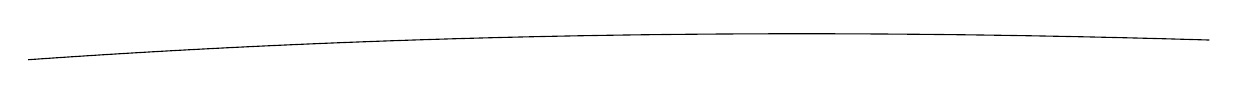
\begin{tikzpicture}\draw (0,0) .. controls (5,.35) and (10,.4) .. (15,.25);\end{tikzpicture}}

\diagram{
\begin{tikzcd}[column sep=small,row sep=small]
\unsure{\Gamma|\mathcal T}_{1,\nu}^{!+}\arrow[r] & \cdots &
\unsure{\Gamma|\mathcal T}_{1,3}^{!+}\arrow[r] &
\unsure{\Gamma|\mathcal T}_{1,2}^{!+}\arrow[r] &
\unsure{\Gamma|\mathcal T}_{1,1}^{!+}\arrow[d,equal]\\
&&\cup&\cup&\operatorname{SL}(2,\mathbb Z)\\
\Pi_{1,\nu-1}&&\Pi_{1,2}&\Pi_{1,1}&\cup\\
\cup&&\cup&\cup&L_0^{\unsure{\widetilde G}}\\
L_0^{(1,\nu-1)}&&L_0^{(1,2)}&L_0^{(1,1)}&
\end{tikzcd}
}

\margin{dans $\unsure{\Gamma|\mathcal T}_{1,\nu}^{!+}$ $(\nu\geq1)$ s-gr
can. \deleted{\unsure{nilpotents}} comm. \deleted{$\unsure{\mathbb Z}$}
de rang $\nu$}

\figure{\begin{tikzpicture}\draw (0,0) -- (14,.7);\end{tikzpicture}}

\margin{$g\geq2,\ \nu\geq0$}

\diagram{
\begin{tikzcd}[column sep=small,row sep=small]
\unsure{\Gamma|\mathcal T}_{g,\nu}^{\unsure{!+1|!+}}\arrow[r] & \overset{\unsure{\wedge}}{\cdots} &
\unsure{\Gamma|\mathcal T}_{g,2}^{!+}\arrow[r,no head] &
\unsure{\Gamma|\mathcal T}_{g,1}^{!+}\arrow[r,no head] &
\unsure{\Gamma|\mathcal T}_{g,0}^{!+}\\
\cup&&\cup&\cup&\cup\\
\Pi_{g,\nu-1}&\cdots&\Pi_{g,1}&\Pi_g&
\unsure{\mathbb Z_g|Z_g}\simeq\mathbb Z^g\\
\cup&&\cup&\cup&\\
L_0^{(g,\nu-1)}&&L_0^{(g,1)}&\Lambda_g\ (\simeq\mathbb Z)&\\
&&&?&
\end{tikzcd}
}

\margin{s-groupes canoniques \deleted{\unsure{nilpotents}}
\unsure{comm.} de rang $\deleted{\unsure{2}}g+\nu$}

\[
\deleted{\unsure{1+2+\cdots+(\nu-1)\leq\frac{(\nu-1)\nu}{2}}}
\]

\margin{180}
\scanpage{181}

\begin{center}
U N I V E R S I T E\\
DES SCIENCES ET TECHNIQUES\\
DU LANGUEDOC\\
\rule{2.8cm}{.4pt}\\
MA/FP
\end{center}
\uline{Diffusion} : Liste A\\
N° 3109

\begin{center}
\uline{AVIS DE SOUTENANCE D'UNE THESE DE DOCTEUR DE}\\
\uline{3ème CYCLE : TECTONIQUE-GEOPHYSIQUE- GEOCHIMIE}
\end{center}

\uline{Nom et Prénom du candidat} : RISPOLI René

\uline{Titre de la thèse} : Microtectonique et champ de contraintes dans les calcaires fins du Languedoc. Exemple des Matelles et du Cirque de Navacelles.

\uline{Date, heure et lieu de soutenance prévus} : 9 Juin 1981, 10h 30, Salle de Cours n° 6\\
U.S.T.L.

\uline{Nom du Directeur de thèse} : MM. les Professeurs MATTAUER, PROUST.

\uline{Désignation du laboratoire où la thèse est préparée} : Laboratoire de Géologie Structurale.

\uline{Analyse de l'ouvrage} : Aux Matelles (20 Km) au Nord de Montpellier, l'observation des microstructures tectoniques pyrénéennes dans les calcaires permet de décrire la géométrie du champ des contraintes et plus particulièrement les concentrations et déviations de $\sigma_1$, $\sigma_2$, $\sigma_3$. On propose à partir de ces données des modèles évolutifs pour les fentes, stylolites et failles. Ces microstructures s'associent entre elles dans les systèmes en échelon qui sont des cisaillements potentiels. Leur description fournit des renseignements sur leur fonctionnement mécanique.

Sur le site du Cirques de Navacelles (Causse du Larzac) la déformation tectonique pyrénéenne est observée. Deux phases de distension mésozoïques sont décrites. L'utilisation de l'analyse numérique des microfailles permet de définir la variation de $\mathrm R=\sigma_2-\sigma_3\,/\,\sigma_1-\sigma_3$ avec la profondeur z. L'utilisation des modèles de contraintes dans la croûte permet d'évaluer la poussée tectonique pyrénéenne entre 100 et 200 bars.

\uline{Durée approximative des recherches ayant abouti à la thèse} : 3 ans.

\uline{Composition du jury proposé} :

\begin{flushleft}
M. MATTAUER M\\
M. PROUST F.\\
M. ARTHAUD F\\
M. ETCHECOPAR A.\\
M. VASSEUR G.
\end{flushleft}

\begin{flushright}
p. Le Secrétaire Général\\
L'Attachée d'Administration Universitaire,\\
\uline{\unsure{Gentil}}\\
A. GENTIL.
\end{flushright}

\margin{181}
\scanpage{182}

\margin{$g,\nu$}

$X$ \uline{propre}

1°) Connexe, lisse \inserted{\unsure{sauf}} pts doubles ordinaires
\inserted{(diviseur $D$)}, dim $1$

2°) $\chi(\deleted{\unsure{X,}}\underline{\mathcal O}_X)\deleted{\unsure{g}}=1-g$

i.e. si $\widetilde X^{\unsure{*|+}}$ la \unsure{normalisée}, $g_i$ les genres,
$\mu$ le nb des pts doubles
\[
g-1=\sum(g_i-1)+\mu
\]
\[
g=\sum g_i+\mu+1-s
\]

\margin{$s$ nb de comp. irr.\\
$\mu$ \rule{1.8cm}{.4pt} pts doubles\\
(\uline{NB} on a tjrs $\mu+1-s\geq0$\\
à cause connexité)}

\margin{
\figure{
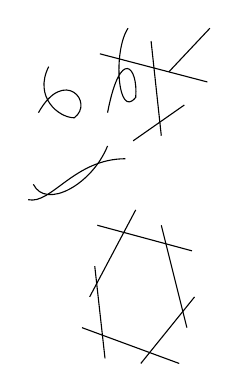
\begin{tikzpicture}[x=.65cm,y=.65cm]
\draw (.1,3.8) .. controls (-.2,3.2) and (.3,2.8) .. (.6,2.8)
 .. controls (1,3.1) and (.4,3.8) .. (-.1,2.9);
\draw (1.25,2.9) .. controls (1.5,4.2) and (1.85,3.8) .. (1.8,3.2)
 .. controls (1.45,2.75) and (1.35,4.1) .. (1.65,4.55);
\draw (1.1,4.05) -- (3.2,3.5);
\draw (2.1,4.3) -- (2.3,2.45);
\draw (2.45,3.7) -- (3.25,4.55);
\draw (1.75,2.35) -- (2.75,3.05);
\draw (-.2,1.5) .. controls (.05,1) and (.95,1.5) .. (1.25,2.25);
\draw (-.3,1.2) .. controls (.15,1.1) and (.6,2.0) .. (1.6,2.0);
\draw (1.05,.7) -- (2.9,.2);
\draw (1.8,1) -- (.9,-.7);
\draw (1,-.1) -- (1.2,-1.9);
\draw (.75,-1.3) -- (2.65,-2.0);
\draw (1.9,-2.0) -- (2.95,-.7);
\draw (2.3,.7) -- (2.8,-1.3);
\end{tikzpicture}
}}

3°) $S\subset X$ \deleted{\unsure{fini|un}} \deleted{\unsure{multisecti.} étale diviseur}
\inserted{sous-schéma. fini étale, de rang $\nu$}
contenu dans l'\unsure{ouv.} des pts de lissité de $X$

4°) Si $X_i$ comp. irréd. \deleted{de genre} \inserted{avec}
$\widetilde X_i$ genre $1$, alors $X_i$ contient un
pt double \uline{ou} \deleted{\unsure{un}} $X_i\cap S\neq\varnothing$
i.e. $X_i\cap(D\cup S)\neq\varnothing$
($\Longleftrightarrow$ \unsure{Exclu ici.}
pour $X$ lisse de genre $1$, $S=\varnothing$)

5°) Si $X_i$ comp. irréd. avec $\widetilde X_i$ de
genre $0$, alors l'image inverse de $(D\cup S)$ dans
$\widetilde X_i$ a au moins trois pts.

\margin{\figure{\begin{tikzpicture}\draw (.2,0) .. controls (-.1,.1) and (0,1) .. (-.1,1.5) .. controls (-.3,1.7) and (-.1,1.75) .. (-.1,2) -- (-.1,3.2);\end{tikzpicture}}\unsure{pas d'autom. inf. de la} ``situation''}

\figure{\begin{tikzpicture}\draw (0,0) -- (15,1.2);\end{tikzpicture}}

\diagram{
\begin{tikzcd}[column sep=small,row sep=small]
\widetilde D\arrow[r,phantom,"\subset"]\arrow[ddr,"\mathrm{surj}"']&
\underbrace{\widetilde D\amalg S}\arrow[r,"\mathrm{surj}"]\arrow[d,phantom,"\unsure{\wr}"]&
\pi_0(\widetilde X)\arrow[r,"\uline{g}"]\arrow[d,equal]&\mathbb N\\
&\widetilde\Delta&\Delta&\\
&D&&
\end{tikzcd}
}

\margin{$\widetilde D\longrightarrow D$ fibres de $\operatorname{card}\leq2$}

\diagram{
\begin{array}{l}
\left\{
\begin{array}{l}
\operatorname{card}S=\textcircled{$\nu$}\\[2pt]
\displaystyle\sum_{\delta\in\Delta}(g_\delta-1)
+\underbrace{\mu}_{\operatorname{card}\widetilde D}
=\textcircled{$g$}\unsure{+|-}1\\[4pt]
\operatorname{card}\bigl(\unsure{\widetilde D|D}\amalg_{\widetilde D}\Delta\bigr)=1\\
\deleted{\text{fibres de }\widetilde D\longrightarrow\Delta
\text{ de }\operatorname{card}\leq2}
\end{array}\right.
\end{array}
}

\margin{182}
\scanpage{183}

maquette de $X$ (sur $k$ alg. clos)

\[
\begin{aligned}
\widetilde D&=\text{image inv. de }D\text{ dans }\widetilde X\\
\widetilde S&=\rule{3.7cm}{.4pt}\ S\text{ dans }\widetilde X
\qquad(\text{NB }\widetilde S\xrightarrow{\sim}S)\\
\Delta&=\pi_0(\widetilde X)\simeq\text{ens des comp. irréd. de }X\\
D&=(\text{pour mémoire})\text{ ens des pts doubles}
\end{aligned}
\]

\diagram{
$\Sigma\left\{\vphantom{\begin{matrix}a\\a\\a\\a\end{matrix}}\right.$
\begin{tikzcd}[column sep=small,row sep=large]
\widetilde D\arrow[r,phantom,"\overset{\unsure{\mathrm{can}}}{\subset}"]
 \arrow[dr,"q\ (\mathrm{surj})"']&
\widetilde D\amalg\widetilde S\arrow[r,"p\ (\mathrm{surj})"]&
\Delta\arrow[r,"\uline{g}"]&\mathbb N\\
&D&&
\end{tikzcd}
}

a) $D\amalg_{\widetilde D}\Delta$ de card. $1$

b) \deleted{les fibres de $q:\widetilde D\to D$ de card $\leq2$}
\inserted{$q$, de degré $2$}

c) $\displaystyle\sum_{\delta\in\Delta}(\uline{g}(\delta)-1)
+\underbrace{\operatorname{card}\overset{\deleted{\unsure{\sim}}}{D}}_{\mu}
=\textcircled{$g$}-1$

d) $\operatorname{card}\widetilde S=\textcircled{$\nu$}$

e) Si $\delta\in\Delta$ tel que $g(\delta)=1$, alors
$p^{-1}(\delta)\neq\varnothing$
($\Longleftrightarrow$ on n'a pas
$\widetilde D=\widetilde S=\varnothing,\ \Delta\unsure{=}\unsure{\{\delta\}},
\ \uline{g}(\delta)=1$)

f) Si $\delta\in\Delta$ tel que $g(\delta)=0$, alors
$\unsure{\operatorname{card}}p^{-1}(\delta)\geq3$

\[
\mu(\Sigma)=\sum_{\delta\in\Delta}\mu(\delta,\Sigma)
\]
où $\mu(\delta,\Sigma)$ ne dépend que de
$\uline{g}(\delta)\overset{\mathrm{def}}=g_\delta$, et de
$\operatorname{card}(p^{-1}(\delta))\overset{\mathrm{def}}=\nu_\delta$,
\[
\begin{aligned}
\mu(\delta,\Sigma)&=
\deleted{\unsure{\xi(g_\delta)}}
\mu(g_\delta,\nu_\delta)
\overset{\mathrm{def}}=
\deleted{\Big\{}
\begin{matrix}
3(g_\delta-1)+\nu_\delta&
\deleted{\text{si }g_\delta\geq1}\\
\deleted{\unsure{\nu_\delta}}&
\deleted{\text{si }g_\delta\unsure{\leq|\geq}1}
\end{matrix}
\end{aligned}
\]
\[
\begin{aligned}
\unsure{\mu}(\Sigma)
&=\sum_\delta\mu(\delta,\Sigma)
=3\sum(g_\delta-1)
+\underbrace{\sum\nu_\delta}_{
\underbrace{\operatorname{card}\widetilde D}_{2\mu}
+\underbrace{\operatorname{card}\widetilde S}_{\nu}}
=3\sum(g_\delta-1)+2\mu+\nu\\
&=3\underbrace{\left(\sum_\delta(g_\delta-1)+\mu\right)}_{g-1}
+\nu-\mu
=\underbrace{(3(g-1)+\nu)}_{\mu(g,\nu)}-\mu
=\mu(g,\nu)-\mu
\end{aligned}
\]

\margin{183}
\scanpage{184}

UNIVERSITE DES SCIENCES\\
ET TECHNIQUES DU LANGUEDOC
\hfill SESSION DE JUIN 1981

\begin{center}
D.E.U.G. A 1ère Année - Maths Appliquées\\
(Séries I et II)

Epreuve d'Analyse - Durée 3 heures

I
\end{center}

On donne l'équation différentielle
\[
xyy'+2y^2=\frac{1}{\unsure{x}^3(x+1)^2}
\]

1 - Déterminer la solution de cette équation définie sur l'intervalle $]1,+\infty[$
et qui prend la valeur $-\frac{1}{4\sqrt3}$ pour $x=2$.

On pourra poser $y^2=z$.

2 - Soit A un nombre réel ; $A>1$. Calculer l'intégrale
\[
\mathrm F(A)=\int_1^A\frac{1}{x^2}\sqrt{\frac{x-1}{x+1}}\,\mathrm dx
\]
\unsure{On pourra poser} $x\unsure{=}\frac1u$ \unsure{et utiliser} la relation
\[
\sqrt{\frac{1-u}{1+u}}=\frac{1-u}{\sqrt{1-u^2}}
\]

3 - Etudier la limite de $\mathrm F(A)$ lorsque A tend vers $+\infty$.

\begin{center}II\end{center}

Etude de la courbe définie paramétriquement par les équations
\[
x=\frac{t(3t^2-2)}{1-t^2}
\qquad
y=\frac{t^4}{1-t^2}
\]

1 - Montrer qu'il suffit d'étudier l'arc obtenu pour $t\in[0,+\infty[$,
l'ensemble de la courbe pouvant s'en déduire par une symétrie.

2 - Calculer les dérivées $\frac{\mathrm dx}{\mathrm dt}$, $\frac{\mathrm dy}{\mathrm dt}$.
Vérifier que ces deux dérivées s'annulent pour $t=\sqrt2$.
Etablir le tableau donnant les variations de x et de y en fonction de t.

3 - Etude de la courbe au voisinage de l'origine.

4 - Etude de la \unsure{branche} infinie obtenue lorsque t tend vers 1.

5 - Etude de la branche infinie obtenue lorsque t tend vers $+\infty$.

On pourra chercher les parties entières de x et de y considérées
comme fractions rationnelles de t et en déduire une parabole asymptotique à la
courbe.

6 - Etude de la courbe au voisinage du point $t=\sqrt2$.

7 - Dessin de la courbe entière.

\begin{center}\rule{1.5cm}{.4pt}\end{center}

\margin{184}
\cotefile{148}
\scanpage{1}

\figure{
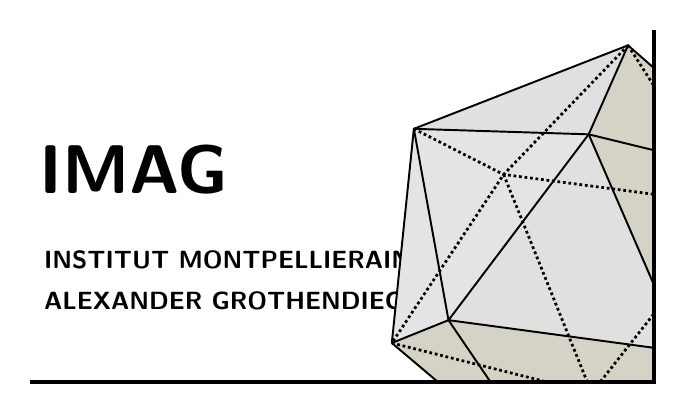
\begin{tikzpicture}[x=1cm,y=1cm]
\node[anchor=west,font=\sffamily\bfseries\fontsize{58}{62}\selectfont] at (.1,-1.9) {IMAG};
\node[anchor=west,font=\sffamily\bfseries\small] at (.16,-3.05) {INSTITUT MONTPELLIERAIN};
\node[anchor=west,font=\sffamily\bfseries\small] at (.16,-3.56) {ALEXANDER GROTHENDIECK};
\begin{scope}
\clip (4.65,-4.60) rectangle (8.03,-.10);
\fill[gray!24] (4.98,-1.38)--(7.70,-.32)--(7.2,-1.45)--cycle;
\fill[yellow!15!gray!45] (7.70,-.32)--(8.02,-.60)--(8.02,-1.65)--(7.2,-1.45)--cycle;
\fill[blue!4!gray!20] (4.98,-1.38)--(7.2,-1.45)--(5.42,-3.81)--(4.70,-4.10)--cycle;
\fill[gray!24] (7.2,-1.45)--(8.02,-3.34)--(8.02,-4.16)--(5.42,-3.81)--cycle;
\fill[yellow!15!gray!45] (7.2,-1.45)--(8.02,-1.65)--(8.02,-3.34)--cycle;
\fill[yellow!15!gray!45] (4.70,-4.10)--(5.42,-3.81)--(8.02,-4.16)--(8.02,-4.59)--(5.28,-4.59)--cycle;
\draw[line width=.7pt] (4.70,-4.10)--(4.98,-1.38)--(7.70,-.32)--(8.02,-.60);
\draw[line width=.7pt] (4.98,-1.38)--(7.2,-1.45)--(8.02,-1.65);
\draw[line width=.7pt] (7.70,-.32)--(7.2,-1.45)--(8.02,-3.34);
\draw[line width=.7pt] (7.2,-1.45)--(5.42,-3.81)--(8.02,-4.16);
\draw[line width=.7pt] (4.98,-1.38)--(5.42,-3.81)--(5.95,-4.59);
\draw[line width=.7pt] (4.70,-4.10)--(5.42,-3.81);
\draw[line width=.7pt] (4.70,-4.10)--(5.28,-4.59);
\draw[densely dotted,line width=1pt] (4.98,-1.38)--(6.12,-1.96)--(8.02,-2.21);
\draw[densely dotted,line width=1pt] (7.70,-.32)--(6.12,-1.96)--(4.70,-4.10);
\draw[densely dotted,line width=1pt] (6.12,-1.96)--(7.18,-4.59);
\draw[densely dotted,line width=1pt] (4.70,-4.10)--(6.65,-4.59);
\draw[densely dotted,line width=1pt] (7.35,-4.59)--(8.02,-3.74);
\draw[densely dotted,line width=1pt] (7.70,-.32)--(8.02,-.82);
\end{scope}
\draw[line width=1.4pt] (.1,-4.60)--(8.03,-4.60)--(8.03,-.12);
\end{tikzpicture}
}
\scanpage{2}

\margin{(29.11.83)}

Soit $X$ surf. à bord compacte orientée, à structure torique
\inserted{(i.e. torseur sous $\mathbb U=\{z\in\mathbb C\mid |z|=1\}$)}
donnée sur les comp. connexes du bord.
On définit
\[
\begin{aligned}
\operatorname{SRT}(\unsure{X})={}&
\text{quotient du groupe des autom de }X
\text{ (\deleted{\unsure{en}} resp. l'orientation}\\
&\text{et les structures toriques) par la comp. neutre du}\\
&\text{sous-groupe }\operatorname{Aut}^!(\vec X)
\deleted{\unsure{\mathrm{bijec.}}}
\text{ de Aut qui induit}\\
&\text{l'identité sur }\partial X
\end{aligned}
\]

On a ainsi un \unsure{dévissage} de $\operatorname{SRT}(X)$ en trois étages
\[
\underbrace{S_{\unsure{*}}T^!(X)}_{
\operatorname{Aut}^!(\unsure{\vec X|\overline X})/
\text{comp. neutre}}
\qquad\mathbb U^I\qquad\unsure{\mathfrak S_I}
\qquad I=\pi_0(\partial X)
\]
ou encore
\[
\mathbb Z^I\qquad T(X)\qquad\mathbb U^I\qquad\unsure{\mathfrak S_I}
\]

En fait, on définit can! un sous-groupe \inserted{droit}
$\mathbb R^I$ de $\operatorname{SRT}(X)$
contenant $\mathbb Z^I$, de telle façon qu'on ait
\[
\underbrace{\operatorname{SRT}^!(X)}_{
\substack{\text{noyau de}\\
\operatorname{SRT}^!(\unsure{X|\alpha})\to\unsure{\mathfrak S_I^!|\mathfrak S_I'}}}
=\mathbb R^I.S_*T^!(X)
\]

\diagram{
\begin{tikzcd}[column sep=small,row sep=large]
\mathbb R^I &
\mathord{:}\arrow[l,phantom,"\subset"']\arrow[dr,no head,"\unsure{\lambda}"] &&\\
\mathbb Z^I\arrow[u,"\unsure{\mathrm{can}}"']\arrow[r,hook]&
S_*T^!\arrow[u,hook]\arrow[r,phantom,"\subset"]&
\operatorname{SRT}^!\arrow[r,phantom,"\subset"]&
\operatorname{SRT}
\end{tikzcd}
}
\margin{\deleted{\unsure{et propre}}}

i.e. on a

\margin{\uline{NB} $\operatorname{SUT}(X)\simeq
T(X)\times\underset{\operatorname{Aut}((T_i)_{i\in I})}{\unsure{\mathfrak S_I}}$}

\margin{\unsure{jusqu'ici on ne fait intervenir}
que $S_*T^!(X)$; à l'exclusion de $S_*T(X)$,
dont la défini. exige une str. suppl.
$\uline{s}$, cf ci-dessous}

\diagram{
\begin{tikzcd}[column sep=small,row sep=large]
&\operatorname{SRT}(X)\arrow[d,no head,"\unsure{\mathfrak S_I}"]&\\
&\mathbb R^I.\unsure{S_*T^!}\arrow[dl,no head,"T^!"']
 \arrow[dr,no head,"\mathbb U^I"]&\\
\mathbb R^I\arrow[dr,no head,"\mathbb U^I"']&&S_*T^!(X)\\
&\mathbb Z^I\arrow[ur,"T^!(X)"']&
\end{tikzcd}
}
\margin{$T(X)\left\{\vphantom{\begin{matrix}a\\a\\a\end{matrix}}\right.$}
\margin{$\left.\vphantom{\begin{matrix}a\\a\\a\end{matrix}}\right\}\operatorname{Aut}((T_i)_{i\in I})$}

d'où
\diagram{
\begin{tikzcd}[row sep=large,column sep=small]
\operatorname{SRT}\deleted{\unsure{(X)}}/\mathbb Z^I
 \overset{\mathrm{def}}=\operatorname{SUT}(X)
 \arrow[d,"\unsure{\mathfrak S_I}"]\\
T^!(X)\times\mathbb U^I
\end{tikzcd}
}
\[
(*)\qquad1\longrightarrow\mathbb U^I\longrightarrow
\operatorname{SUT}(X)-\unsure{T|\Gamma}(X)-1
\]

De plus, chaque fois qu'on se donne un
marquage, i.e. un pt \deleted{\unsure{de}}
\[
\uline{s}=(s_i)\in
\prod_{i\in I=\pi_0(\partial X)}
\deleted{\unsure{\mathbb U_i}}T_i
\]
\margin{$T_i=$ comp. connexe (torique) de $\partial X$ d'indice $i$}

on trouve un plongement
\[
S_*T^{\unsure{!}}(X,\uline{s})\hookrightarrow\operatorname{SRT}(X)
\]
tel qu'on en déduise
\[
S_*T^{\unsure{!}}(X,\uline{s})
\mathbin{\wedge}_{\mathbb Z^I}\mathbb R^I
\simeq\operatorname{SRT}(X)
\]

\margin{1}
\scanpage{3}

Une façon de le voir est de dire que
la donnée de $\uline{s}$ définit un scindage
\inserted{$\varphi_{\uline{s}}$} de
l'extension $(*)$ ci-dessus, et que \unsure{vu pour}
ss-groupe de $\operatorname{SRT}(X)$,
$S_{\unsure{1|*}}T(X,\uline{s})$ s'identifie
à l'image inverse de
\[
\varphi_{\uline{s}}(T(X))\subset\operatorname{SUT}(X)
\]
par l'hom. can
\[
\operatorname{SUR}(X)\longrightarrow\operatorname{SUT}(X)
\]
de passage au quotient. Le chgt de
$\uline{s}$ en $\uline{s}'=u.\uline{s}$
transforme $\varphi_{\uline{s}}$ en
\[
\varphi_{\uline{s}'}=\operatorname{int}(u)\circ\varphi_{\uline{s}}
\]
donc si $\widetilde u\in\mathbb R^I$ relève $u$, on trouve
\[
S_{\unsure{1|*}}T(X,\uline{s}')
=\operatorname{int}(\widetilde u)S_{\unsure{1|*}}T(X,\uline{s}).
\]

En termes de $\vec X$, la définition de
$S_{\unsure{1|*}}T(X,\uline{s})$
dépend d'un choix $\uline{s}$ \uline{non-anodin},
par contre celle de $S_1RT(X)$ ne dépend que d'
un choix anodin, celui de la famille des
structures toriques $(t_i)_{i\in I}$.
De plus $\prod T_i$ comme
torseur sous $\unsure{\mathbb U^I}$ se réalise
\inserted{(pas fidèlement d'ailleurs)}
comme une classe de scindages de l'ext $(*)$
(via autom. int. par $\mathbb U^I$)
$\bigl[$\unsure{déduits} de $\operatorname{SRT}(X)$
avec \unsure{ses} structures suppl.$\bigr\}$
savoir les inclusions

\diagram{
\begin{tikzcd}[row sep=small]
\mathbb R^I\arrow[dr] &\\
&\operatorname{SRT}(X)\\
S_{\unsure{1|*}}T^!(X)\arrow[ur]&
\end{tikzcd}
}

\unsure{coïncid.} sur $\mathbb Z^I$.

\margin{2}
\scanpage{4}

Ceci dit, si on se donne un
multimarquage de $\partial X$, savoir pour
chaque $i\in I$ un $n_i\in\mathbb N^*$ et un
sous-\inserted{$\mathbb U_{n_i}$-}torseur
$T_i(n_i)\subset T_i$,
\deleted{\unsure{les groupes}} i.e.
un $s_i\in T_i^{\wedge n_i}$, d'où
$\deleted{\unsure{\uline{s}\in}}$
\[
\uline{s}\in\prod_{i\in I}T_i^{\wedge n_i},
\]
alors le groupe de Teichmüller \unsure{multimarqué}
$S_{\unsure{*|1}}T(\unsure{X},\uline{s})$,
généralisant le précédent, est
plongé dans $\operatorname{SRT}(X)$ de façon naturelle,
en prenant un $s_i^0$ dans chaque $T_i(n_i)$, d'où
$\uline{s}^0\in\prod T_i$ et
$ST(X,\uline{s}^0)\subset\operatorname{SRT}(X)$,
et on prend le ss-groupe
\[
ST(X,\uline{s})=ST(X,\uline{s}^0).
\prod_{i\in I}\frac1{n_i}\mathbb Z_i
\]
où $\mathbb Z_i$ est le $i$ème facteur de
$\mathbb Z^I\subset\operatorname{SRT}(X)$.

\margin{3}
\scanpage{5}
\mspage{1}

\uline{Courbes \inserted{exceptionnelles} de type} $(1,1)$ (sur $\mathbb C$)

A) \uline{Courbe \inserted{ell.} anharmonique de type carré}

Cat. de ces courbes \unsure{équivalente} : celle des carrés
\deleted{\unsure{équilatères}} orientés, i.e. des torseurs sur
\[
\mathbb Z/4\mathbb Z\simeq\mu_4(\mathbb C)\simeq
\text{groupe des unités algébriques de }\mathbb Q[i]
\]
\margin{i.e. groupe des unités de $\mathbb Z[i]$
\unsure{anneau} des entiers de $\mathbb Q[i]$}

La donnée d'un tel torseur \inserted{($S$)} permet de tordre
$\mathbb E\ell_0\overset{\mathrm{def}}\simeq
\mathbb C/\mathbb Z[i]$ et trouver
\[
\mathbb E\ell_0(S)\simeq\mathbb E\ell_0
\mathbin{\wedge}_{\mathbb Z/4\mathbb Z}S
\]

\margin{
\figure{
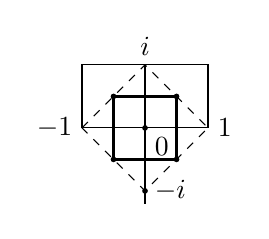
\begin{tikzpicture}[scale=.8]
\draw[thin] (-1,0)--(-1,1)--(1,1)--(1,0);
\draw[dashed] (-1,0)--(0,1)--(1,0)--(0,-1)--cycle;
\draw (-1,0)--(1,0);
\draw (0,-1.2)--(0,1);
\draw[thick] (-.5,-.5)--(-.5,.5)--(.5,.5)--(.5,-.5)--cycle;
\foreach \x/\y in {0/0,-.5/.5,.5/.5,.5/-.5,-.5/-.5,0/-1}
{\fill (\x,\y) circle (.045);}
\node[left] at (-1,0) {$-1$}; \node[right] at (1,0) {$1$};
\node[above] at (0,1) {$i$}; \node[right] at (0,-1) {$-i$};
\node[below right] at (0,0) {$0$};
\end{tikzpicture}
}}

Si le carré est réalisé comme un carré \inserted{au dedans}
dans un plan euclidien \inserted{$V_S$} (canoniquement), de centre $0$,
\deleted{
\figure{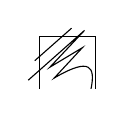
\begin{tikzpicture}[scale=.55]
\draw (0,0)--(0,1.2)--(1.3,1.2)--(1.3,0);
\draw (-.25,.2)--(1.05,1.35)--(.25,.5)--(1,.95)--(.35,.25)
 .. controls (1.2,.75) and (1.3,.5) .. (1.2,0);
\draw (-.1,.65)--(.75,1.4);
\end{tikzpicture}}
}
\figure{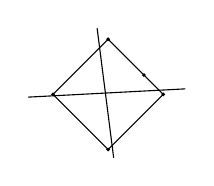
\begin{tikzpicture}[scale=.7]
\draw (-1,0)--(0,1)--(1,0)--(0,-1)--cycle;
\draw (-1.45,-.05)--(1.4,.1); \draw (.1,-1.15)--(-.2,1.2);
\foreach \x/\y in {-1/0,0/1,1/0,0/-1,.65/.35}
{\fill (\x,\y) circle (.035);}
\end{tikzpicture}}
on en déduit dans le plan (vectoriel via $0$) $V_S$
un syst. de deux \deleted{axes de}
coordonnées \inserted{mod. signes}
via les diagonales, d'où un
\deleted{\unsure{lattice}} \inserted{réseau}
$\Gamma_S$ dans $V_S$ (sous-groupe discret de
rang $2$) et
\[
\boxed{\mathbb E\ell_0(\unsure{S})\unsure{\simeq|/2}
X_S=V_S/\Gamma_S}.
\]

\margin{
\figure{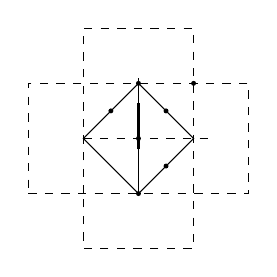
\begin{tikzpicture}[scale=.7]
\draw[dashed] (-1,-1)--(-1,2)--(1,2)--(1,-2)--(-1,-2)--(-1,-1);
\draw[dashed] (-2,-1)--(2,-1)--(2,1)--(-2,1)--cycle;
\draw (-1,0)--(0,1)--(1,0)--(0,-1)--cycle;
\draw[dashed] (-1,0)--(1.4,0);
\draw (0,-1)--(0,1.1);
\draw[very thick] (0,-.2)--(0,.65);
\foreach \x/\y in {0/0,0/1,0/-1,-.5/.5,.5/.5,.5/-.5,1/1}
{\fill (\x,\y) circle (.045);}
\end{tikzpicture}}
}

Il y a dans $X_S$ un élément d'ordre $2$ canonique
\inserted{$\unsure{\eta_S}$}
(stable par automorphismes), les deux autres él. d'
ordre $2$ sont échangés par le générateur $i$ de
$\mu_4(\mathbb C)\simeq\operatorname{Aut}(\unsure{X_S})$.
(\uline{NB} $\unsure{\eta_S}$ peut donc être défini

\margin{4}
\scanpage{6}

\begin{center}
U N I V E R S I T E\\
DES SCIENCES ET TECHNIQUES\\
DU LANGUEDOC\\
\textasciicircum\textasciicircum\textasciicircum\textasciicircum\textasciicircum\textasciicircum\textasciicircum\textasciicircum\textasciicircum\textasciicircum\textasciicircum\textasciicircum\textasciicircum
\end{center}

Montpellier, le 14 octobre 1983

Service de la Scolarité

Diffusion : Liste A\\
MA/gs \hfill N° 4375

\begin{center}
AVIS DE SOUTENANCE D'UNE THESE DE DOCTORAT DE 3e CYCLE

\uuline{ECOLOGIE GENERALE ET APPLIQUEE OPTION ECOLOGIE AQUATIQUE}
\end{center}

\uline{NOM et Prénom du candidat} : MONTI Dominique

\uline{Titre de la thèse} : ``Recherches sur l'optimisation du plan d'échantillonnage employé pour la cartographie des peuplements benthiques. Application à la macrofaune benthique de l'étang de Pierre Blanche (Palavas, Hérault, France).

\uline{Date,-heure et lieu de soutenance prévus} : Le 2 novembre 1983 à 15 heures,\\
Salle de cours n° 9 - Université des Sciences et Techniques du Languedoc

\uline{Nom du Directeur de thèse} : M. AMANIEU

\uline{Désignation du Laboratoire où la thèse est préparée} : Laboratoire d'Hydrobiologie marine - U.S.T.L.

\uline{Analyse de l'ouvrage} : Cette réflexion porte sur le problème du choix du nombre et de l'organisation spatiale des points de prélèvement en écologie. Quel effort doit-on fournir pour un niveau de précision fixé ? Et où doit-on prélever ?

Ce travail est basé sur la réalisation de différents sous-échantillonnages d'une information initiale supposée maximale. Les différents sous-échantillonnages varient par le nombre et l'organisation spatiale des points de prélèvements ; et ils sont tous effectués à partir de la même liste d'objets.

Chaque sous-échantillonnage employé donnera naissance à une carte qui sera par la suite comparée à la carte dite ``de référence'' ; il restera à apprécier au vu de ces résultats si les cartes obtenues diffèrent de la référence, en quelles proportions et de quelle manière.

Les résultats théoriques sont appliqués à l'étude de la macrofaune benthique d'un étang littoral (l'étang de Pierre Blanche à Palavas, France).

\uline{Durée approximative des recherches ayant abouti à la thèse} : 3 ans

\uline{Composition du jury Proposé} : \begin{tabular}[t]{ll}
MM. & AMANIEU M.\\
& BLANC F.\\
& FRONTIER S.\\
& GRANDJOUAN G.\\
& LASSERRE G.
\end{tabular}

\begin{flushright}
P/ le Secrétaire Général,\\
L'Attachée Principale d'Administration\\
Scolaire et Universitaire,

\unsure{A. Gentil}

A. GENTIL
\end{flushright}

\margin{5}
\scanpage{7}
\mspage{2}

comme l'unique élément de \({}_2(X_S)\) qui est fixe par $\operatorname{Aut}(X_S)\simeq\mathbb Z/4\mathbb Z$. En fait
\inserted{\[
(X_S)^{\unsure{i}}\overset{\unsure{\mathrm{def}}}{\unsure{=}}\{x\in X_S\deleted{\}} \mid ix=x\}=\{e,\eta_S\}
\]}
\deleted{\unsure{$X$}} La surface top. $X_S$ a une déc. cell. \inserted{\unsure{can.}} \inserted{\unsure{can. Aut.}} avec 1 sommet $e$, deux arêtes, une face, correspondant aux deux mailles du réseau $\Gamma_S$.

On considère $X_S$ comme muni de cette décomposition. Parfois c'est l'image inv. de celle-ci par $2\operatorname{id}_{X_S}$ qui est plus commode, 4 sommets (formant \({}_2(X_S)\)), \deleted{quatre} \inserted{huit} arêtes, \deleted{(\uline{NB} \unsure{le}} \inserted{4} faces. On peut considérer $\mathbb Z/4\mathbb Z\simeq\mu_4(\mathbb C)$ comme le groupe d'automorphismes commun de ces deux structures cellulaires.

\figure{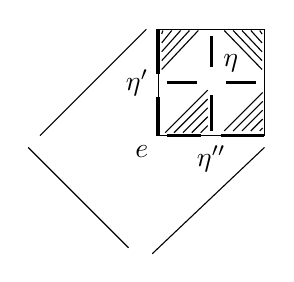
\begin{tikzpicture}[scale=.75]
\draw (-2,0)--(-.2,1.8);
\draw (-2.2,-.2)--(-.5,-1.9);
\draw (-.1,-2)--(1.8,-.2);
\draw (0,0) rectangle (1.8,1.8);
\draw[densely dashed] (0,1.8)--(1.8,1.8)--(1.8,0);
\draw[line width=1.2pt] (0,0)--(0,.65) (0,1.05)--(0,1.8) (.15,0)--(.72,0) (1.06,0)--(1.8,0);
\draw[line width=1.2pt] (.9,.08)--(.9,.69) (.9,1.16)--(.9,1.68) (.15,.9)--(.65,.9) (1.15,.9)--(1.65,.9);
\foreach \t in {.12,.27,.42,.57,.72}{
 \draw[thin] (\t,.05)--(.84,.89-\t);
 \draw[thin] (.06,1+\t)--(.8-\t,1.78);
 \draw[thin] (1+\t,1.78)--(1.76,1+\t);
 \draw[thin] (1+\t,.08)--(1.77,.85-\t);
}
\node[below left] at (0,0) {$e$};
\node[left] at (0,.9) {$\eta'$};
\node[below] at (.9,0) {$\eta''$};
\node[above right] at (.94,.92) {$\unsure{\eta}$};
\end{tikzpicture}}

La deuxième est mieux adaptée pour la description du quotient
\[
\deleted{\unsure{X}\mathbb E\ell(\unsure{S})}\quad X_S/\pm1
\]
qui est une sphère, subdivisée en \deleted{deux} \inserted{faces} \unsure{carrés}, se raccordant suivant un équateur \deleted{carré}, subdivisé en quatre arêtes par $e^{\unsure{\natural}},\eta^{\unsure{\natural}},\eta'^{\unsure{\natural}},\eta''^{\unsure{\natural}}$.

\figure{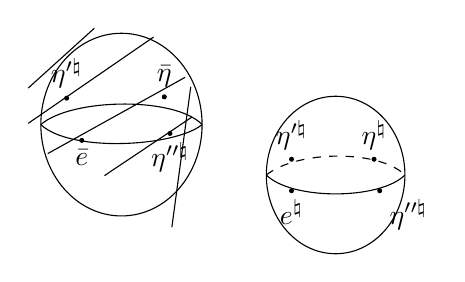
\begin{tikzpicture}[scale=.8]
\begin{scope}
\draw (0,0) ellipse (1.28 and 1.45);
\draw (-1.28,0) .. controls (-.8,.42) and (.85,.45) .. (1.28,0);
\draw (-1.28,0) .. controls (-.8,-.45) and (.85,-.35) .. (1.28,0);
\fill (-.63,-.25) circle (.04) node[below] {$\unsure{\bar e}$};
\fill (-.87,.42) circle (.04) node[above] {$\unsure{\eta'^\natural}$};
\fill (.68,.44) circle (.04) node[above] {$\unsure{\bar\eta}$};
\fill (.77,-.14) circle (.04) node[below] {$\unsure{\eta''^\natural}$};
\draw (-1.48,.58)--(-.43,1.53) (-1.48,.02)--(.51,1.39) (-1.17,-.46)--(1.01,.75) (-.27,-.81)--(1.12,.12) (1.1,.6)--(.8,-1.63);
\end{scope}
\begin{scope}[xshift=3.4cm,yshift=-.8cm]
\draw (0,0) ellipse (1.1 and 1.25);
\draw[dashed] (-1.1,0) .. controls (-.6,.4) and (.7,.4) .. (1.1,0);
\draw (-1.1,0) .. controls (-.7,-.4) and (.7,-.4) .. (1.1,0);
\fill (-.7,.25) circle (.04) node[above] {$\unsure{\eta'^\natural}$};
\fill (.61,.25) circle (.04) node[above] {$\unsure{\eta^\natural}$};
\fill (-.7,-.25) circle (.04) node[below] {$\unsure{e^\natural}$};
\fill (.7,-.25) circle (.04) node[below right] {$\unsure{\eta''^\natural}$};
\end{scope}
\end{tikzpicture}}

\margin{6}
\scanpage{8}

\begin{center}
U N I V E R S I T E\\
DES SCIENCES ET TECHNIQUES\\
\uline{DU LANGUEDOC}

Service de la Scolarité\\
MA/GJ\\
Diffusion : Liste A\\
N° : 4679
\end{center}

Montpellier, le 20 octobre 1983

\begin{center}
\uline{AVIS DE SOUTENANCE D'UNE THESE DE DOCTEUR INGENIEUR}

\uline{AUTOMATIQUE}
\end{center}

\uline{Nom et prénom du candidat} : SITOHANG Benhard

\uline{Titre de la thèse} : LINAIRE : SYSTEME DE GESTION DE BASES DE DONNEES RELATIONNELLES SUR MICRO-ORDINATEUR.

\uline{Date, heure et lieu de soutenance prévus:} 28 OCTOBRE 1983 à 14h30 - CRIG USTL

\uline{Nom du Directeur de thèse} : Monsieur le Professeur B. FILLIATRE

\uline{Désignation du laboratoire où la thèse est préparée} : CRIG USTL

\uline{Résumé de la thèse} :

La conception et la réalisation d'un Système de Gestion de Bases de Données Relationnelles sur micro-ordinateur, que nous avons baptisé ``LINAIRE'', est le sujet de cette thèse.

Nous mettons l'accent sur trois points principaux :

1. BOUCLE MULTI-NIVEAUX ; c'est une technique du traitement de données, permettant d'éviter l'utilisation des relations intermédiaires comme résultats des opérateurs relationnels, ce qui serait particulièrement pénalisant pour un micro-ordinateur possédant une mémoire centrale limitée.

2. STRUCTURE INTERNE DE LA BASE ; elle est multiple, afin de préserver au mieux les performances tout en offrant en particulier la possibilité d'accélérer le traitement de l'opérateur relationnel ``équi-joint''.

3. L'adaptation sur un micro-ordinateur du langage de manipulation de QUERY-BY-EXAMPLE (langage de haut niveau, interactif, et tabulaire).

\uline{Durée approximative des recherches ayant abouti à la thèse} : 2 ans

\uline{Composition du jury proposé} :

\begin{tabular}{ll}
MM. & FILLIATRE B.\\
& CHEIN M.\\
& PICHAT E.\\
& PIROTTE A.\\
& PRUNET F.
\end{tabular}

\begin{center}
P. le Secrétaire Général,\\
l'Attachée Principale d'Administration Scolaire\\
et Universitaire,

\unsure{A. Gentil}

A. GENTIL
\end{center}

\margin{7}
\scanpage{9}
\mspage{3}

B) Courbes \inserted{ell.} \unsure{anharmoniques} de type hexagonal.

La catégorie de ces courbes équivaut à celle des hexagones orientés, i.e. des torseurs $S$ sous
\[
\begin{aligned}
\mathbb Z/6\mathbb Z&\simeq\mu_6(\mathbb C)\simeq
\text{groupe des unités \inserted{\unsure{alg.}} de }Q(\underbrace{\sqrt[3]{1}}_{\zeta})\\
&\simeq\text{groupe des unités de}\\
&\qquad \deleted{\mathbb Z[\zeta]\unsure{=}\mathbb Z[T]/}\\
&\qquad \mathbb Z[\zeta]=\mathbb Z[T]/(1+T+T^2)\\
&\qquad (\zeta\unsure{=|:}\exp 2i\pi/3)
\end{aligned}
\]

\figure{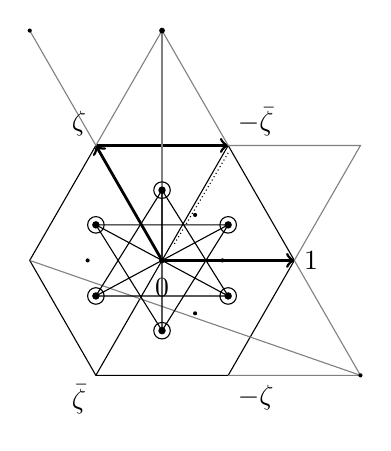
\begin{tikzpicture}[scale=1.05]
\coordinate (O) at (0,0);
\coordinate (A) at (1.6,0);
\coordinate (B) at (.8,1.39);
\coordinate (C) at (-.8,1.39);
\coordinate (D) at (-1.6,0);
\coordinate (E) at (-.8,-1.39);
\coordinate (F) at (.8,-1.39);
\draw (A)--(B)--(C)--(D)--(E)--(F)--cycle;
\draw[line width=1pt,->] (O)--(A);
\draw[line width=1pt,->] (O)--(C);
\draw[line width=1pt,->] (C)--(B);
\draw (E)--(O)--(B);
\draw[densely dotted] (.15,.2)--(.8,1.3);
\draw[thin,gray] (-1.6,2.78)--(C)--(0,2.78)--(B);
\draw[thin,gray] (0,2.78)--(0,0);
\draw[thin,gray] (A)--(2.4,-1.39)--(F);
\draw[thin,gray] (D)--(2.4,-1.39);
\draw[thin,gray] (A)--(2.4,1.39)--(B);
\fill (0,2.78) circle (.035);
\fill (-1.6,2.78) circle (.025);
\fill (2.4,-1.39) circle (.025);
\foreach \p in {(0,.85),(.8,.43),(.8,-.43),(0,-.85),(-.8,-.43),(-.8,.43)}{
 \draw \p circle (.10);
 \fill \p circle (.045);
}
\draw[thin] (0,.85)--(.8,-.43)--(-.8,-.43)--cycle;
\draw[thin] (0,-.85)--(.8,.43)--(-.8,.43)--cycle;
\draw[thin] (0,.85)--(0,-.85) (-.8,.43)--(.8,-.43) (-.8,-.43)--(.8,.43);
\foreach \p in {(-.9,0),(.73,0),(.4,.55),(.4,-.64)}\fill \p circle (.025);
\fill (O) circle (.035);
\node[below] at (0,-.10) {$\unsure{0}$};
\node[right] at (A) {$1$};
\node[above left] at (C) {$\zeta$};
\node[above right] at (B) {$-\bar\zeta$};
\node[below left] at (E) {$\bar\zeta$};
\node[below right] at (F) {$-\zeta$};
\end{tikzpicture}}

\deleted{\unsure{On pourra}} \inserted{On pose}
\[
\mathbb E\ell_1\deleted{(\unsure{S})}\simeq\mathbb C/\mathbb Z[\zeta]
\]
\[
\mathbb E\ell_1(S)\simeq\mathbb E\ell_1\mathbin{\wedge}_{\mathbb Z/6\mathbb Z}S
\]

\uline{Construction} On réalise l'hexagone orient. $S$ \unsure{euclidiennement} (canonique), \unsure{dans} \unsure{vectoriel} euclidien $V_S$, \deleted{\unsure{centre}} \inserted{origine} étant le barycentre de $S$. On désigne par $\unsure{V_S|\Gamma_S}$ le \deleted{\unsure{lattice}} \inserted{réseau} engendré par $S$, et
\[
X_S=\mathbb E\ell_1(S)\simeq V_S/\Gamma_S
\]
La structure euclidienne \uline{orientée} de $V_S$ définit la structure complexe de $X_S$.

\margin{8}
\scanpage{10}

\begin{center}
U N I V E R S I T E\\
DES SCIENCES ET TECHNIQUES\\
DU LANGUEDOC\\
\textasciicircum\textasciicircum\textasciicircum\textasciicircum\textasciicircum\textasciicircum\textasciicircum\textasciicircum\textasciicircum\textasciicircum\textasciicircum\textasciicircum\textasciicircum
\end{center}

Montpellier, le 18 octobre 1983

Service de la Scolarité

Diffusion : Liste A\\
AM/gs \hfill N° 4570

\begin{center}
AVIS DE SOUTENANCE D'UNE THESE DE DOCTEUR-INGENIEUR

\uuline{``ECOLOGIE GENERALE ET APPLIQUEE option ECOLOGIE TERRESTRE''}
\end{center}

\uline{NOM et prénom du candidat} : MOUFADDAL Mohamed

\uline{Titre de la thèse} : ``CONTRIBUTION A L'ETUDE DES POSSIBILITES D'EXTENSION DU CEDRE DE L'ATLAS EN DEHORS DE SON AIRE ACTUELLE''

\uline{Date, heure et lieu de soutenance prévus} : Le 28 octobre 1983 à 14 heures à l'Institut de Botanique

\uline{Nom du directeur de thèse} : M. GODRON Michel

\uline{Désignation du laboratoire où la thèse est préparée} : Centre d'Etudes Phytosociologiques et écologiques Louis Emberger (CNRS)

\uline{Aanlyse de l'ouvrage} : L'objet de cette étude étant de cerner les possibilités d'extension du Cèdre (\uline{Cedrus atlantica} Manetti) en dehors de son aire actuelle, il a fallu, après une analyse de l'histoire de répartition du Cèdre, préciser les facteurs climatiques responsables de la distribution actuelle.

Les régions où l'introduction du Cèdre est possible, sont déterminées à partir de l'étude climatique de stations situées à l'intérieur et à l'extérieur de l'aire du Cèdre, et par une étude écologique et dendrométrique comparative de quelques plantations.

\uline{Durée approximative des recherches ayant abouti à la thèse} : 5 ans

\uline{Composition du jury proposé} : \begin{tabular}[t]{ll}
MM. & GODRON M.\\
& BEDEL J.\\
& SCHOENENBERGER A.\\
& ROMANE F.\\
& DAGET Ph.
\end{tabular}

\begin{flushright}
P/ le Secrétaire Général,\\
l'Attachée principale d'administration\\
scolaire et universitaire,

\unsure{A. Gentil}

\uline{A. GENTIL}
\end{flushright}

\margin{9}
\scanpage{11}
\mspage{4}

Le groupe $\mathbb Z/6\mathbb Z$ opère transitivement sur $({}_2X_S)\setminus\{0\}$ car $\pm1$ opère trivialt - donc \({}_2X_S\setminus\{0\}\) est un torseur sous
\[
(\mathbb Z/6\mathbb Z)/\pm1\simeq\mathbb Z/3\mathbb Z
\]
\deleted{(\unsure{conj.}} (générateur canonique $\unsure{\simeq}\,-\bar\zeta\,\unsure{j}=\exp\frac{2\pi}{6}$),
\deleted{\unsure{en ce cas}} \inserted{le torseur} s'identifie \unsure{:|à} $S/\pm1$, en associant à chaque $s\in S$ le milieu du rayon $[0,s]$, ou plutôt son image dans $X_S$.

L'ens des pts fixes de $\mathbb Z/3\mathbb Z\inserted{\subset\mathbb Z/6\mathbb Z}$ sur $X_S$ est de card 3, il s'obtient en prenant les barycentres des six triangles de la subdivision centrale (\unsure{bibarycentrique}) de l'hexagone (pts cerclés) (tels que $(1-\bar\zeta)/3$ etc dans le cas épinglé), ils se groupent en deux paquets de 3 \unsure{mutuellement} congrus \unsure{sous|mod} $\Gamma$, \unsure{donnant|donnent} deux éléments (symétriques) de $X_S$, d'ordre 3,

\margin{10}
\scanpage{12}

\begin{center}
U N I V E R S I T E\\
DES SCIENCES ET TECHNIQUES\\
DU LANGUEDOC\\
\textasciicircum\textasciicircum\textasciicircum\textasciicircum\textasciicircum\textasciicircum\textasciicircum\textasciicircum\textasciicircum\textasciicircum\textasciicircum\textasciicircum\textasciicircum
\end{center}

Montpellier, le 14 octobre 1983

Service de la Scolarité

Diffusion : Liste A\\
MA/gs \hfill N° 4470

\begin{center}
AVIS DE SOUTENANCE D'UNE THESE DE DOCTEUR-INGENIEUR

\uuline{`` PHYSIQUE DES MATERIAUX ''}
\end{center}

\uline{NOM et Prénom du candidat} : GOUDEAU Jacques

\uline{Titre de la thèse} : ``Contraintes de trempe thermique dans des pièces à symétrie de révolution''

\uline{Date, heure et lieu de soutenance prévus} : Le 28 octobre 1983, à 11 heures\\
Salle de l'IREM - Université des Sciences et Techniques du Languedoc

\uline{Nom du Directeur de thèse} : M. ZARZYCKI - M. MAISONNEUVE

\uline{Désignation du Laboratoire où la thèse est préparée} : Laboratoire de Sciences des Matériaux, Mécanique des Milieux continus, Chimie structurale - U.S.T.L.

\uline{Analyse de l'ouvrage} : On étudie l'évolution des champs de température et de contraintes, dans une pièce en verre à symétrie de révolution.

Pour cela on résout par éléments finis un problème de thermovisco-élasticité, avec une loi de comportement de type MAXWELL à coefficients variables en fonction de la température.

On compare les résultats obtenus à ceux d'une méthode optique d'analyse des contraintes ainsi qu'à une méthode industrielle de mésure.

\uline{Durée approximative des recherches ayant abouti à la thèse} : 2 ans

\uline{Composition du jury proposé} : \begin{tabular}[t]{ll}
MM. & ZARZYCKI J.\\
& MAISONNEUVE O.\\
& REGNIER J\\
& FRANCOIS\\
& BOURRET D.
\end{tabular}

\begin{flushright}
P/ le Secrétaire Général,\\
l'Attachée Principale d'Administration\\
Scolaire et Universitaire,

\unsure{A. Gentil}

\uline{A. GENTIL}
\end{flushright}

\margin{11}
\scanpage{13}
\mspage{5}

qui avec l'origine $e$ forment l'ens des pts fixes de $X_S$. (L'ens des pts fixes sous $\mathbb Z/6\mathbb Z$ est réduit à $e$.) Les deux pts fixes sous $\mathbb Z/3\mathbb Z$, distincts de $e$, correspondent aux deux triangles \unsure{co-inscrits|coinscrits} de l'hexagone $S$. (\inserted{les deux} triplets des côtés mutuellement non adjacents.)

\uline{Décompositions cellulaires canoniques.} Décomposition en deux faces triangulaires, par trois arêtes, un seul sommet. Les faces triangulaires correspondent aux éléments de $(X_S)^\zeta\setminus\{e\}$ (chaque face en contient un et un seul) i.e. aux triangles \unsure{co-inscrits|coinscrits} de l'hexagone. Les côtés correspondent aux trois

\margin{12}
\scanpage{14}

\begin{center}
U N I V E R S I T E\\
DES SCIENCES ET TECHNIQUES\\
\uline{DU LANGUEDOC}

Service de la Scolarité\\
MA/GJ\\
Diffusion : Liste A\\
N°: 4680
\end{center}

Montpellier, le 20 octobre 1983

\begin{center}
\uline{AVIS DE SOUTENANCE D'UNE THESE DE DOCTORAT DE 3ème CYCLE}

\uline{EVOLUTION ET BIOSYSTEMATIQUE}
\end{center}

\uline{Nom et prénom de la candidate} : CHAKROUN Saïda

\uline{Titre de la thèse} : LES VARIATIONS SAISONNIERES DES FORMATIONS SECONDAIRES (BOIS, LIBER, CAMBIUM) DU TRONC DE TROIS ESPECES MEDITERRANEENNES, LE CHENE VERT, L'OLIVIER, ET LE MICOCOULIER : UNE ETUDE HISTOPHYSIOLOGIQUE.

\uline{Date, heure et lieu de soutenance prévus} : 28 Octobre 1983 à 9h30\\
Salle de Cours n°9 - U.S.T.L.

\uline{Nom des Directeurs de thèse} : MM. Charles HEBANT et BONNET

\uline{Désignation du laboratoire où la thèse est préparée} : Laboratoire de Biologie Végétale

\uline{Résumé de la thèse} :

Cette étude concerne l'anatomie, l'histologie et l'histochimie des tissus conducteurs secondaires d'\textit{Olea europaea}, de \textit{Quercus ilex}, et de \textit{Celtis australis}.

Le bois et le liber du Chêne et de l'Olivier ont fait l'objet d'une étude structurale approfondie.

Le fonctionnement de la zone cambiale (ainsi que la mise en place de ses dérivés, bois et liber) et l'évolution des réserves amylacées du tronc de ces trois espèces subissent des variations importantes avec le rythme saisonnier, et dans le cas de l'Olivier, avec les alternances de production.

Chez le Chêne et le Micocoulier, la totalité du bois et du liber est différenciée au printemps et en été. Chez l'Olivier, la réactivation cambiale au printemps est plus ou moins précoce selon la charge en fruits ; de plus, seuls les arbres en faible production montrent une reprise d'activité cambiale en automne, cette dernière engendre uniquement du bois.

Chez les trois espèces, la mise en place du liber est initiée plus tardivement que dans le cas du bois. Chez les deux espèces à feuilles persistantes, la zone du liber conducteur ne disparaît jamais, par contre, chez le Micocoulier, à la fin de l'automne et pendant l'hiver, tous les tubes criblés deviennent non conducteurs en accumulant de la callose.

Parallèlement à la réactivation cambiale, on note une hydrolyse de l'amidon. L'amylogénèse est plus ou moins précoce selon l'espèce observée, et dans le cas de l'Olivier, selon la charge en fruits. Une compétition entre la croissance végétative et le développement reproductif de l'Olivier est observée.

Tout au long de l'année, les cellules compagnes et les rayons vasculaires du Chêne et de l'Olivier possèdent une forte activité phosphohydrolasique et respiratoire.

\uline{Durée approximative des recherches ayant abouti à la thèse} : 3 ans

\uline{Composition du jury proposée} :

\begin{tabular}{ll}
MM. & D'AUZAC J.\\
& BONNET A.L.\\
& KAUMAN W.\\
& NABLI M.A\\
& THALER L.\\
& VILLEMUR P.
\end{tabular}

\begin{center}
P. le Secrétaire Général,\\
l'Attachée Principale d'Administration Scolaire\\
et Universitaire,

\unsure{A. Gentil}

A. GENTIL
\end{center}

\margin{13}
\scanpage{15}
\mspage{6}

diagonales de l'hexagone, ou encore aux trois pts d'ordre 2 distincts de $e$.

Ici encore on peut ``doubler'' la décomposition cellulaire, et en \unsure{tirer} une autre avec 4 sommets, \deleted{\unsure{8|6}} \inserted{\unsure{12}} arêtes, et 8 faces (triangulaires), qui permet de mieux comprendre le passage au quotient par $\pm1$, avec quatre sommets (dont un sommet privilégié, correspondant à $e$),

\figure{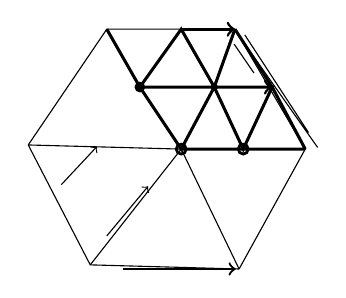
\begin{tikzpicture}[scale=1.05]
\coordinate (L) at (-1.85,0);
\coordinate (UL) at (-.9,1.4);
\coordinate (UR) at (.65,1.4);
\coordinate (R) at (1.5,-.05);
\coordinate (LR) at (.7,-1.5);
\coordinate (LL) at (-1.1,-1.45);
\coordinate (O) at (0,-.05);
\coordinate (T) at (0,1.4);
\coordinate (P) at (-.5,.7);
\coordinate (Q) at (.4,.7);
\coordinate (V) at (1.1,.7);
\coordinate (W) at (.75,-.05);
\draw (L)--(UL)--(UR)--(R)--(LR);
\draw (LR)--(LL)--(L);
\draw (L)--(O)--(LL) (O)--(LR);
\draw[line width=1.1pt] (UL)--(P)--(O)--(Q)--(UR);
\draw[line width=1.1pt] (P)--(T)--(Q)--(W)--(V)--(Q)--(P);
\draw[line width=1.1pt] (O)--(W)--(R) (UR)--(V)--(R);
\draw[->,line width=1pt] (T)--(UR);
\draw[->,line width=1pt] (Q)--(V);
\draw[->] (-1.45,-.48)--(-1.02,-.02);
\draw[->] (-.9,-1.1)--(-.4,-.5);
\draw[->,line width=.8pt] (-.7,-1.5)--(.66,-1.5);
\draw[thin] (.70,1.32)--(1.65,-.03) (.77,1.33)--(1.54,.15) (.64,1.22)--(.88,.87);
\fill (P) circle (.065);
\fill (Q) circle (.045);
\draw[line width=1pt] (O) circle (.06) (W) circle (.06);
\end{tikzpicture}}

six arêtes les reliant $2\unsure{:|à}2$ : c'est la structure tétraédrique \inserted{(orientée)}, avec un sommet fixé, groupe \unsure{d'automorphismes|d'automorphisme} $\mathbb Z/3\mathbb Z$ (\deleted{\unsure{pourtant}} $\simeq\mathbb Z/6\mathbb Z\,/\pm1$, OK !).

\margin{14}
\scanpage{16}

\begin{center}
U N I V E R S I T E\\
DES SCIENCES ET TECHNIQUES\\
DU LANGUEDOC\\
\textasciicircum\textasciicircum\textasciicircum\textasciicircum\textasciicircum\textasciicircum\textasciicircum\textasciicircum\textasciicircum\textasciicircum\textasciicircum\textasciicircum\textasciicircum
\end{center}

Montpellier, le 14 octobre 1983

Service de la Scolarité

Diffusion : Liste A\\
MA/gs \hfill N° 4469

\begin{center}
AVIS DE SOUTENANCE D'UNE THESE DE DOCTORAT DE 3e CYCLE

\uuline{`` SCIENCES AGRONOMIQUES option PHYTOTECHNIE ''}
\end{center}

\uline{NOM et Prénom du candidat} : LECONTE Antoine

\uline{Titre de la Thèse} : ``LA REPRODUCTION SEXUEE DE L'HEVEA BRASILIENSIS (UNE APPROCHE HISTOLOGIQUE ET EXPERIMENTALE)''

\uline{Date, heure et lieu de soutenance prévus} : 27 octobre 1983 à 9h.30 - Salle de cours n°9 - (Bât. administratif ) Université des Sciences et Techniques du Languedoc.

\uline{Nom du Directeur de thèse} : MM. Charles HEBANT - BONNET

\uline{Désignation du laboratoire où la thèse est préparée} : Laboratoire de Biologie végétale - U.S.T.L.

\uline{Analyse de l'ouvrage} : L'amélioration génétique de l'Hévéa est entravée par un très mauvais taux de réussite des pollinisations contrôlées.

L'étude histologique montre que le processus reproducteur (gaméto-génèse, fécondation et développement embryonnaire) se déroule normalement. Une exception est signalée : le cas du clone GT 1 dont la stérilité mâle est décrite. La fécondation a lieu moins de 24 heures après la pollinisation.

L'étude expérimentale, menée en Côte d'Ivoire, porte sur les modalités de la floraison et de la fructification en conditions naturelles et artificielles. La majorité des fleurs subissent une élimination naturelle dans un délai de 5 à 15 jours après la pollinisation. Des traitements hormonaux (ANA, chlorure de cobalt) peuvent augmenter significativement le taux de fructification.

Une explication physiologique de la faible fertilité de l'Hévéa est proposée.

\uline{Durée approximative des recherches ayant abouti à la thèse} : 2 ans

\uline{Composition du jury proposé} : \begin{tabular}[t]{ll}
MM. & BONNET\\
& D'AUZAC\\
& HALLE\\
& NICOLAS D.
\end{tabular}

\begin{flushright}
P/ le Secrétaire Général,\\
l'Attachée Principale d'Administration scolaire et universitaire,

\unsure{A. Gentil}

\uline{A. GENTIL}
\end{flushright}

\margin{15}
\scanpage{17}

\[
M_{\unsure{0\,4|0,4}}
\]

\[
M_{1,1}
\]

\margin{16}
\scanpage{18}

$4$ sommets d'ordre $6$ $+6$ sommets d'ordre $6$ $+12$ sommets d'ordre $3$

$24$ triangles $+4$ hexagones

\figure{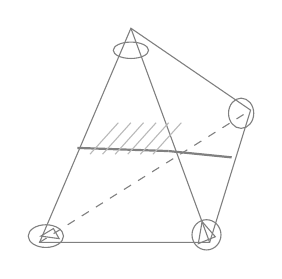
\begin{tikzpicture}[scale=0.8]
\draw[gray] (0,0)--(1.45,3.4)--(3.35,2.1)--(2.7,0)--cycle;
\draw[gray] (1.45,3.4)--(2.7,0);
\draw[dashed,gray] (0,0)--(3.35,2.1);
\draw[gray,thick] (0.6,1.5)--(2.05,1.45);
\draw[gray,thick] (2.05,1.45)--(3.05,1.35);
\draw[gray] (1.45,3.05) ellipse (0.28 and 0.13);
\draw[gray] (0.1,0.1) ellipse (0.28 and 0.18);
\draw[gray] (2.65,0.12) ellipse (0.23 and 0.24);
\draw[gray] (3.2,2.05) ellipse (0.2 and 0.24);
\draw[gray,thin] (0.02,0.1)--(0.22,0.22)--(0.31,0.06)--cycle;
\draw[gray,thin] (2.52,-0.02)--(2.58,0.33)--(2.79,0.09)--cycle;
\foreach \x in {0.8,1,1.2,1.4,1.6,1.8}{\draw[gray!55] (\x,1.4)--(\x+0.45,1.9);}
\end{tikzpicture}}

\figure{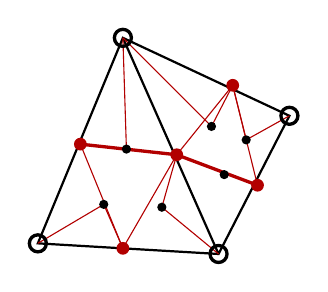
\begin{tikzpicture}[scale=0.9]
\coordinate (A) at (0,0); \coordinate (B) at (1.2,2.9);
\coordinate (C) at (2.55,-0.15); \coordinate (D) at (3.55,1.8);
\draw[thick] (A)--(B)--(D)--(C)--cycle (B)--(C);
\draw[red!70!black,very thick] (0.6,1.4)--(1.96,1.25)--(3.1,0.82);
\draw[red!70!black] (B)--(1.25,1.33) (0.6,1.4)--(1.2,-0.07)--(1.96,1.25)--(2.75,2.23)--(3.1,0.82);
\draw[red!70!black] (A)--(0.93,0.55)--(1.2,-0.07) (C)--(1.75,0.51)--(1.96,1.25);
\draw[red!70!black] (B)--(2.45,1.65)--(2.75,2.23) (D)--(2.94,1.46)--(2.75,2.23);
\foreach \p in {A,B,C,D}{\draw[very thick] (\p) circle (0.12);}
\foreach \p in {(0.6,1.4),(1.96,1.25),(3.1,0.82),(1.2,-0.07),(2.75,2.23)}{\fill[red!70!black] \p circle (0.09);}
\foreach \p in {(1.25,1.33),(0.93,0.55),(1.75,0.51),(2.45,1.65),(2.94,1.46),(2.63,0.97)}{\fill \p circle (0.065);}
\end{tikzpicture}}

\margin{\unsure{voir aussi} cf verso (\unsure{barycentres de} \unsure{triangulation})}

\[
\begin{aligned}
s_0&=4+6+4.3=22\\
s_1&=12+4.\unsure{8|9}=48\\
s_2&=4.7=28
\end{aligned}
\]

\figure{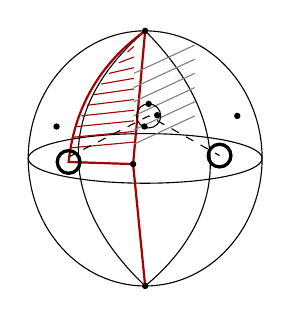
\begin{tikzpicture}[scale=0.9]
\draw (0,0) ellipse (1.65 and 1.8);
\draw (0,0) ellipse (1.65 and 0.35);
\draw (0,1.8) .. controls (-1.45,0.55) and (-1.05,-0.8) .. (0,-1.8);
\draw (0,1.8) .. controls (1.3,0.5) and (1.15,-0.85) .. (0,-1.8);
\draw[red!65!black,thick] (0,1.8)--(-0.17,-0.08)--(0,-1.8);
\draw[red!65!black,thick] (0,1.8) .. controls (-0.8,1.22) and (-1.02,0.5) .. (-1.08,-0.05)--(-0.17,-0.08);
\foreach \y/\x in {0.15/-1.04,0.3/-1.01,0.45/-0.96,0.6/-0.9,0.75/-0.82,0.9/-0.72,1.05/-0.62,1.2/-0.51,1.35/-0.37,1.5/-0.25}{\draw[red!65!black] (\x,\y)--(-0.16,\y+0.08);}
\foreach \y in {0.2,0.4,0.6,0.8,1,1.2}{\draw[gray] (-0.16,\y)--(0.7,\y+0.4);}
\draw[very thick] (-1.08,-0.05) circle (0.16) (1.05,0.04) circle (0.16);
\draw[dashed] (-1.08,0.02)--(0.05,0.6)--(1.05,0.04);
\draw (0.05,0.6) circle (0.17);
\foreach \p in {(0,1.8),(0,-1.8),(-1.25,0.45),(1.3,0.6),(-0.17,-0.08),(0.05,0.77),(0.17,0.61),(-0.01,0.45)}{\fill \p circle (0.045);}
\end{tikzpicture}}

\figure{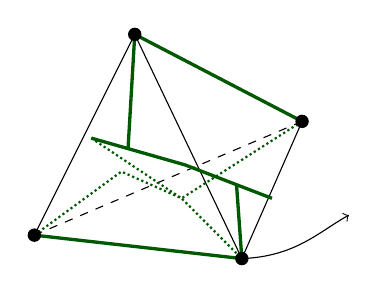
\begin{tikzpicture}[scale=0.85]
\coordinate (A) at (0,0); \coordinate (B) at (1.5,3);
\coordinate (C) at (3.1,-0.35); \coordinate (D) at (4,1.7);
\draw (A)--(B)--(C) (C)--(D);
\draw[green!35!black,very thick] (A)--(C) (B)--(D);
\draw[dashed] (A)--(D);
\draw[green!35!black,very thick] (0.85,1.45)--(2.25,1.05)--(3.55,0.55) (B)--(1.4,1.3) (C)--(3.02,0.76);
\draw[green!35!black,densely dotted,thick] (A)--(1.3,0.95)--(2.2,0.55)--(C);
\draw[green!35!black,densely dotted,thick] (0.85,1.45)--(2.2,0.55)--(D);
\foreach \p in {A,B,C,D}{\fill (\p) circle (0.1);}
\draw[->] (C) .. controls (3.9,-0.32) and (4.25,0.05) .. (4.7,0.3);
\end{tikzpicture}}

\margin{ça fait $2^4-1=15$ \unsure{possibilités} \unsure{d'inversion} \unsure{des faces choisies} \unsure{en} \unsure{des} \unsure{bords} !}

\uline{$4$ types de points-base}

$\bullet$ $3$ structures carrées, sur $I$ (ou $J$)

$\textcolor{red!70!black}{\bullet}$ $2$ structures \unsure{tétraèdres|tétraédriques} $=$ \unsure{orientation des faces}

$\textcolor{red!30!black}{\bullet}$ $6$ structures \inserted{bi}\unsure{pantaloniques} \unsure{appariées|opposées} (maillot ceinturé) (carrée $+$ codiagonale \unsure{$J$} $\simeq$ repère de $J$)

\[
\updownarrow
\]

$\bullet$ $6$ structures pantaloniques de \unsure{quasi-gss} (\unsure{quart de tore})
($\simeq$ carré, $+$ orientation de $I$ i.e. de $J$ $\simeq$ repère de $J$)

\margin{$\omega_I=\unsure{{}^{6J}\omega_J}$}

\diagram{\begin{tikzcd}
\operatorname{rep}(J) \arrow[d,leftrightarrow]\\
J\times\omega_J
\end{tikzcd}}

\figure{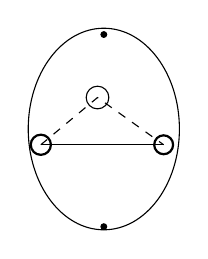
\begin{tikzpicture}[scale=0.8]
\draw (0,0) ellipse (1.2 and 1.6);
\draw (-1,-0.25)--(0.95,-0.25);
\draw[dashed] (-1,-0.25)--(-0.1,0.5)--(0.95,-0.25);
\draw (-0.1,0.5) circle (0.18);
\draw[thick] (-1,-0.25) circle (0.16) (0.95,-0.25) circle (0.15);
\fill (0,1.5) circle (0.055); \fill (0,-1.55) circle (0.055);
\end{tikzpicture}}

\figure{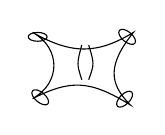
\begin{tikzpicture}[scale=0.8]
\draw (0,0) .. controls (0.45,0.25) and (0.45,0.8) .. (0,1.05)
.. controls (0.65,0.68) and (1.05,0.72) .. (1.6,1.05)
.. controls (1.2,0.55) and (1.2,0.25) .. (1.55,-0.1)
.. controls (0.9,0.3) and (0.6,0.3) .. (0,0);
\draw (0.08,0.98) ellipse (0.15 and 0.07);
\draw[rotate around={-40:(0.12,0.02)}] (0.12,0.02) ellipse (0.16 and 0.08);
\draw[rotate around={-40:(1.5,0.98)}] (1.5,0.98) ellipse (0.16 and 0.08);
\draw[rotate around={45:(1.46,-0.01)}] (1.46,-0.01) ellipse (0.16 and 0.08);
\draw (0.78,0.85)..controls(0.7,0.55)..(0.78,0.3);
\draw (0.89,0.85)..controls(0.98,0.55)..(0.89,0.3);
\end{tikzpicture}}

\margin{sur cette figure, on voit à la fois la \unsure{p.r.q.} du tétraèdre : la configuration-carré, et : la configuration bien \unsure{pantalonnée} du \unsure{quasi-gss}.}

\figure{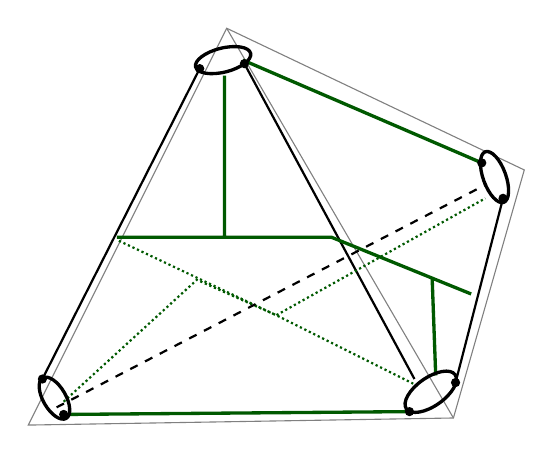
\begin{tikzpicture}[scale=0.9]
\coordinate (A) at (0,0); \coordinate (B) at (2.5,5);
\coordinate (C) at (5.5,0.05); \coordinate (D) at (6.5,3.4);
\draw[thin,gray] (-0.2,-0.15)--(2.6,5.45)--(6.8,3.45)--(5.8,-0.05)--cycle;
\draw[thin,gray] (2.6,5.45)--(5.8,-0.05);
\draw[thick] (0,0.5)--(2.22,4.88) (2.85,4.95)--(5.25,0.5) (5.83,0.45)--(6.5,3.05);
\draw[green!35!black,very thick] (0.32,0)--(5.18,0.04) (2.83,5)--(6.2,3.55);
\draw[green!35!black,very thick] (1.05,2.5)--(4.08,2.5)--(6.05,1.7) (2.57,4.78)--(2.57,2.5) (5.55,0.55)--(5.5,1.92);
\draw[green!35!black,densely dotted,thick] (0.3,0.18)--(2.18,1.9)--(3.3,1.4)--(5.3,0.4);
\draw[green!35!black,densely dotted,thick] (1.08,2.45)--(3.3,1.4)--(6.25,3.05);
\draw[dashed,thick] (0.2,0.1)--(6.27,3.25);
\draw[very thick,rotate around={14:(2.55,5)}] (2.55,5) ellipse (0.4 and 0.17);
\draw[very thick,rotate around={-60:(0.17,0.23)}] (0.17,0.23) ellipse (0.33 and 0.16);
\draw[very thick,rotate around={35:(5.48,0.32)}] (5.48,0.32) ellipse (0.42 and 0.2);
\draw[very thick,rotate around={110:(6.38,3.35)}] (6.38,3.35) ellipse (0.38 and 0.16);
\foreach \p in {(0,0.5),(0.3,0),(2.22,4.88),(2.85,4.95),(5.18,0.04),(5.83,0.45),(6.2,3.55),(6.5,3.05)}{\fill \p circle (0.065);}
\end{tikzpicture}}

\uline{$4$ types de chemins élémentaires}$^{*}$

a) ``\unsure{quart de} twist'' $(2\times3\times4)$ (contour d'un trou)

b) ``sixième de tour'' $(2\times2\times3)$ (sur équateur)

c) pôle vers trou $(2\times2\times3)$ et inv.

d) pôle vers équateur et inv. $(2\times2\times3)$

$2$ types composés supplém.

e) trou vers trou $(2\times3)$ ou ``tiers de tour''

f) demi twist $(2\times2\times3)$

[et bien sûr, g) twist complet $2\times2\times3)$]

\uline{relations} ...

\figure{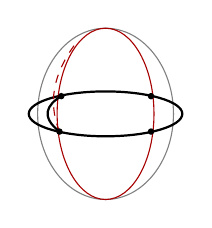
\begin{tikzpicture}[scale=0.75]
\draw[gray] (0,0) ellipse (1.15 and 1.45);
\draw[thick] (0,0) ellipse (1.3 and 0.38);
\draw[red!65!black] (0,0) ellipse (0.82 and 1.45);
\draw[red!65!black,dashed] (-0.78,-0.3)..controls(-1.02,0.3)and(-0.8,0.8)..(-0.5,1.2);
\draw[thick] (-0.78,-0.3)..controls(-1.1,-0.05)and(-1,0.15)..(-0.75,0.3);
\foreach \p in {(-0.78,-0.3),(-0.75,0.3),(0.77,-0.3),(0.77,0.3)}{\fill \p circle (0.055);}
\end{tikzpicture}}

\margin{17}

\margin{$*$ avec les deux sens de parcours, cela fait \uline{huit} types de déformations, à visualiser a) du pt de vue conforme b) du pt de vue combinatoire (ici encore deux pts de vue possibles)}
\scanpage{19}

passage du carré aux deux tétraèdres

\figure{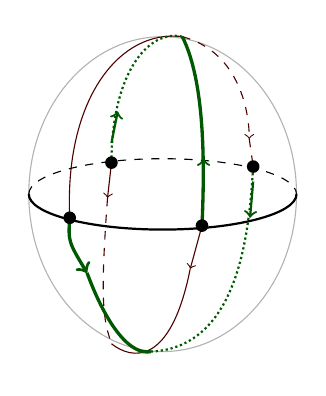
\begin{tikzpicture}[scale=1]
\draw[gray!60] (0,0) ellipse (1.7 and 2);
\draw[thick] (-1.7,0) arc[start angle=180,end angle=360,x radius=1.7,y radius=.45];
\draw[dashed] (-1.7,0) arc[start angle=180,end angle=0,x radius=1.7,y radius=.45];
\draw[red!30!black] (-1.18,-.3)..controls(-1.25,1.2)and(-.55,2.1)..(.25,2);
\draw[red!30!black,dashed,->] (.25,2)..controls(1,1.8)and(1.1,1)..(1.1,.7);
\draw[red!30!black,dashed] (1.1,.7)--(1.15,.35);
\draw[red!30!black,->] (.5,-.4)--(.35,-.95);
\draw[red!30!black] (.35,-.95)..controls(.1,-2.2)and(-.4,-2.1)..(-.65,-1.9);
\draw[red!30!black,->] (-.65,.4)--(-.7,-.05);
\draw[red!30!black,dashed] (-.7,-.05)..controls(-.8,-1.4)and(-.75,-1.6)..(-.65,-1.9);
\draw[green!35!black,very thick] (.25,2)..controls(.55,1.4)and(.53,.3)..(.5,-.4);
\draw[green!35!black,->,thick] (.52,.05)--(.52,.45);
\draw[green!35!black,densely dotted,thick] (-.65,.4)..controls(-.65,1.5)and(-.2,2.1)..(.25,2);
\draw[green!35!black,->,thick] (-.65,.65)--(-.57,1.05);
\draw[green!35!black,very thick,->] (-1.18,-.3)..controls(-1.2,-.6)..(-.96,-1);
\draw[green!35!black,very thick] (-.96,-1)..controls(-.7,-1.7)and(-.4,-2.05)..(-.15,-2);
\draw[green!35!black,densely dotted,thick] (-.15,-2)..controls(1,-1.95)and(1.1,-.4)..(1.15,.35);
\draw[green!35!black,->,thick] (1.15,.16)--(1.11,-.3);
\foreach \p in {(-1.18,-.3),(.5,-.4),(-.65,.4),(1.15,.35)}{\fill \p circle (.08);}
\end{tikzpicture}}

Pour avoir le passage \unsure{aux autres} structures pantaloniques, il faut introduire la \deleted{\unsure{double}}\unsure{subdivision} barycentrique complète de la carte carrée.

dans les deux cas \inserted{``\unsure{spéciaux}''} non dégénérés (carré, tétraèdre) les frontières adjacentes sont \deleted{\unsure{toutes}} ``contenues dans la subdivision barycentrique

\begin{flushright}
\texttt{NS 001 072}\\
\texttt{L ===> PAGE}\\
\texttt{************}
\end{flushright}

\figure{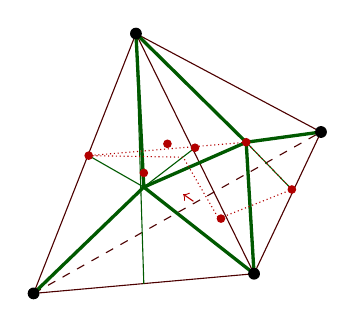
\begin{tikzpicture}[scale=1]
\coordinate (A) at (0,0); \coordinate (B) at (1.3,3.3);
\coordinate (C) at (2.8,.25); \coordinate (D) at (3.65,2.05);
\coordinate (O) at (1.4,1.35); \coordinate (P) at (2.7,1.92);
\draw[red!30!black] (A)--(B)--(C)--(D)--(B);
\draw[red!30!black] (A)--(C);
\draw[red!30!black,dashed] (A)--(D);
\draw[green!35!black,very thick] (B)--(O)--(A) (O)--(C) (O)--(P)--(D) (B)--(P)--(C);
\draw[green!35!black] (B)--(1.4,.12) (.7,1.75)--(O)--(2.05,1.85) (2.7,1.92)--(3.28,1.32);
\draw[red!70!black,densely dotted] (.7,1.75)--(1.9,1.73)--(2.35,.95)--(3.28,1.32)--(2.7,1.92)--cycle;
\foreach \p in {A,B,C,D}{\fill (\p) circle (.075);}
\foreach \p in {(.7,1.75),(1.4,1.53),(2.05,1.85),(2.7,1.92),(3.28,1.32),(1.7,1.9),(2.38,.95)}{\fill[red!70!black] \p circle (.055);}
\draw[red!70!black,->] (2.03,1.17)--(1.9,1.26);
\end{tikzpicture}}

cette carte \inserted{\unsure{commune}} (subdivision bar. du tétraèdre) contient également les subdivisions barycentriques des trois \unsure{coins|cas} ``carrés'' associés, (dont l'une est marquée en pointillés rouges)

\figure{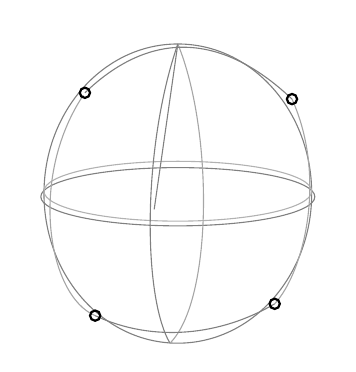
\begin{tikzpicture}[scale=1]
\draw[gray] (0,0) ellipse (1.7 and 1.9);
\draw[gray] (0,-.04) ellipse (1.74 and .37);
\draw[gray!60] (0,.03) ellipse (1.7 and .38);
\draw[gray] (0,1.9)..controls(-.45,.6)and(-.45,-1.3)..(-.1,-1.9);
\draw[gray!70] (0,1.9)..controls(.45,.8)and(.45,-1.35)..(-.1,-1.9);
\draw[gray] (-1.18,1.28)..controls(-.4,2.03)and(.5,2.1)..(1.45,1.2);
\draw[gray] (-1.05,-1.55)..controls(-.3,-1.9)and(.55,-1.8)..(1.23,-1.4);
\draw[gray!70] (-1.2,1.25)..controls(-1.9,.2)and(-1.65,-1.3)..(-1.05,-1.55);
\draw[gray!70] (1.45,1.2)..controls(1.9,.2)and(1.6,-1)..(1.23,-1.4);
\foreach \p in {(-1.18,1.28),(1.45,1.2),(-1.05,-1.55),(1.23,-1.4)}{\draw[thick] \p circle (.065);}
\draw[gray] (0,1.9)--(-.3,-.2);
\end{tikzpicture}}

\margin{18}
\scanpage{20}

\figure{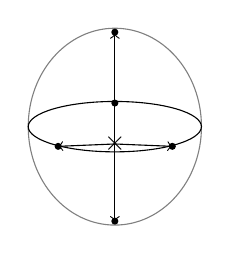
\begin{tikzpicture}[scale=1]
\draw[gray] (0,0) ellipse (1.1 and 1.25);
\draw (0,0) ellipse (1.1 and .32);
\draw[->] (0,-.22)--(0,1.18);
\draw[->] (0,-.22)--(0,-1.2);
\draw[->] (0,-.22)--(-.72,-.25);
\draw[->] (0,-.22)--(.73,-.25);
\node at (0,-.22) {$\times$};
\foreach \p in {(0,1.2),(0,.3),(-.72,-.25),(.73,-.25),(0,-1.2)}{\fill \p circle (.045);}
\end{tikzpicture}}

\figure{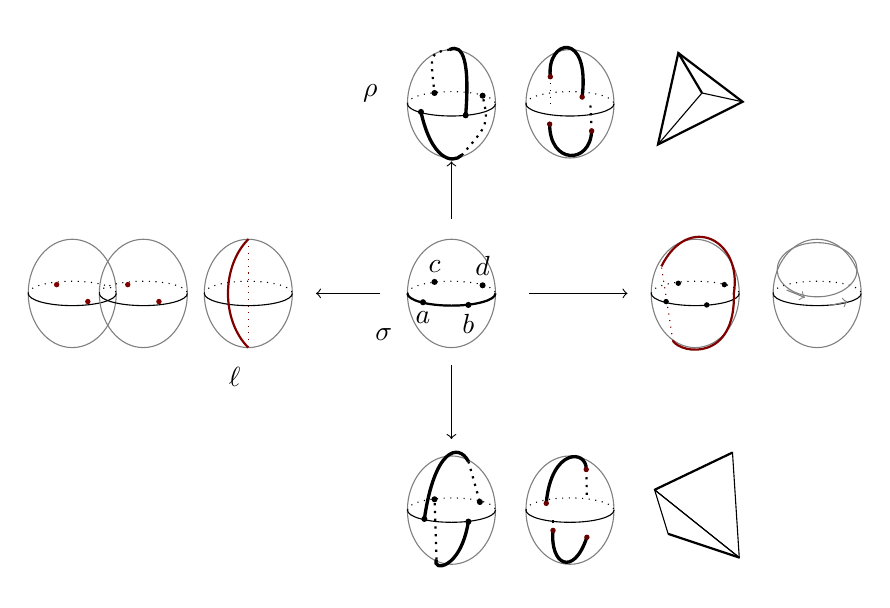
\begin{tikzpicture}[scale=.86]
\foreach \x/\y in {0/0,1.05/0,2.6/0,5.6/0,9.2/0,11/0,5.6/2.8,7.35/2.8,5.6/-3.2,7.35/-3.2}{
\begin{scope}[shift={(\x,\y)}]
\draw[gray] (0,0) ellipse (.65 and .8);
\draw (-.65,0) arc[start angle=180,end angle=360,x radius=.65,y radius=.18];
\draw[dotted] (-.65,0) arc[start angle=180,end angle=0,x radius=.65,y radius=.18];
\end{scope}}
\foreach \x in {0,1.05}{
\fill[red!50!black] (\x-.23,.13) circle (.04);
\fill[red!50!black] (\x+.23,-.12) circle (.04);}
\begin{scope}[shift={(2.6,0)}]
\draw[red!50!black,thick] (0,.8)..controls(-.4,.4)and(-.4,-.4)..(0,-.8);
\draw[red!50!black,dotted] (0,.8)--(0,-.8);
\node[below] at (-.2,-.95) {$\ell$};
\end{scope}
\begin{scope}[shift={(5.6,0)}]
\draw[thick] (-.65,0) arc[start angle=180,end angle=360,x radius=.65,y radius=.18];
\foreach \p in {(-.42,-.13),(.25,-.17),(-.25,.17),(.46,.12)}{\fill \p circle (.045);}
\node[below] at (-.42,-.13) {$a$};
\node[below] at (.25,-.17) {$b$};
\node[above] at (-.25,.17) {$c$};
\node[above] at (.46,.12) {$d$};
\node at (-1,-.6) {$\sigma$};
\end{scope}
\draw[->] (4.55,0)--(3.6,0);
\draw[->] (6.75,0)--(8.2,0);
\draw[->] (5.6,1.1)--(5.6,1.95);
\draw[->] (5.6,-1.05)--(5.6,-2.15);
\begin{scope}[shift={(9.2,0)}]
\draw[red!50!black,thick] (-.5,.4)..controls(-.1,1.2)and(.7,.8)..(.57,0)..controls(.6,-1)and(-.2,-.9)..(-.33,-.7);
\draw[red!50!black,dotted] (-.33,-.7)--(-.5,.4);
\foreach \p in {(-.43,-.12),(.17,-.17),(-.25,.15),(.43,.13)}{\fill \p circle (.04);}
\end{scope}
\begin{scope}[shift={(11,0)}]
\draw[gray] (0,.35) ellipse (.59 and .4);
\draw[->,gray] (-.45,.05)--(-.18,-.06);
\draw[->,gray] (.18,-.18)--(.45,-.12);
\end{scope}
\begin{scope}[shift={(5.6,2.8)}]
\draw[very thick] (-.45,-.12)..controls(-.3,-.8)and(0,-.9)..(.15,-.76);
\draw[dotted,thick] (.15,-.76)..controls(.55,-.3)..(.46,.12);
\draw[very thick] (.21,-.17)..controls(.27,.6)and(.18,.9)..(-.03,.8);
\draw[dotted,thick] (-.03,.8)..controls(-.32,.75)..(-.25,.16);
\foreach \p in {(-.45,-.12),(.21,-.17),(-.25,.16),(.46,.12)}{\fill \p circle (.045);}
\node at (-1.2,.15) {$\rho$};
\end{scope}
\begin{scope}[shift={(7.35,2.8)}]
\draw[very thick] (-.3,-.3)..controls(-.3,-.9)and(.3,-.9)..(.32,-.4);
\draw[dotted,thick] (.32,-.4)--(.3,0);
\draw[very thick] (.18,.1)..controls(.3,1.1)and(-.35,.95)..(-.29,.4);
\draw[dotted] (-.29,.4)--(-.29,0);
\foreach \p in {(-.3,-.3),(.32,-.4),(.18,.1),(-.29,.4)}{\fill[red!40!black] \p circle (.04);}
\end{scope}
\begin{scope}[shift={(9.2,2.8)}]
\draw[thick] (-.55,-.6)--(-.25,.75)--(.7,.03)--cycle;
\draw (-.55,-.6)--(.1,.16)--(.7,.03);
\draw[thick] (-.25,.75)--(.1,.16);
\end{scope}
\begin{scope}[shift={(5.6,-3.2)}]
\draw[very thick] (-.4,-.13)..controls(-.25,.9)and(.1,1)..(.25,.72);
\draw[dotted,thick] (.25,.72)--(.42,.12);
\draw[very thick] (.25,-.17)..controls(.13,-.9)and(-.3,-.9)..(-.22,-.73);
\draw[dotted,thick] (-.22,-.73)--(-.25,.16);
\foreach \p in {(-.4,-.13),(.42,.12),(.25,-.17),(-.25,.16)}{\fill \p circle (.045);}
\end{scope}
\begin{scope}[shift={(7.35,-3.2)}]
\draw[very thick] (-.35,.1)..controls(-.28,.92)and(.25,.9)..(.24,.6);
\draw[dotted,thick] (.24,.6)--(.25,.2);
\draw[very thick] (.25,-.4)..controls(.05,-1)and(-.3,-.8)..(-.25,-.3);
\draw[dotted,thick] (-.25,-.3)--(-.25,-.12);
\foreach \p in {(-.35,.1),(.24,.6),(.25,-.4),(-.25,-.3)}{\fill[red!40!black] \p circle (.04);}
\end{scope}
\begin{scope}[shift={(9.2,-3.2)}]
\draw (-.6,.3)--(.55,.85)--(.65,-.7)--cycle;
\draw[thick] (-.6,.3)--(.55,.85) (-.4,-.35)--(.65,-.7);
\draw (-.6,.3)--(-.4,-.35)--(.65,-.7) (-.6,.3)--(.65,-.7);
\end{scope}
\end{tikzpicture}}

\figure{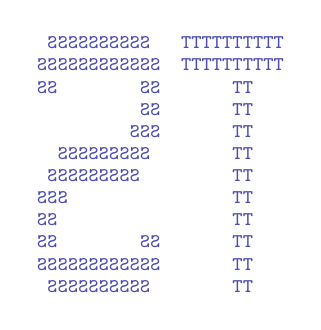
\begin{tikzpicture}
\node[xscale=-1,transform shape,align=left,text=blue!40!gray,font=\ttfamily\scriptsize] {
\unsure{TTTTTTTTTT}\quad\phantom{S}\unsure{SSSSSSSSSS}\phantom{S}\\
\unsure{TTTTTTTTTT}\quad\unsure{SSSSSSSSSSSS}\\
\phantom{TTT}\unsure{TT}\phantom{TTTTT}\quad\unsure{SS}\phantom{SSSSSSSS}\unsure{SS}\\
\phantom{TTT}\unsure{TT}\phantom{TTTTT}\quad\unsure{SS}\phantom{SSSSSSSSSS}\\
\phantom{TTT}\unsure{TT}\phantom{TTTTT}\quad\unsure{SSS}\phantom{SSSSSSSSS}\\
\phantom{TTT}\unsure{TT}\phantom{TTTTT}\quad\phantom{S}\unsure{SSSSSSSSS}\phantom{SS}\\
\phantom{TTT}\unsure{TT}\phantom{TTTTT}\quad\phantom{SS}\unsure{SSSSSSSSS}\phantom{S}\\
\phantom{TTT}\unsure{TT}\phantom{TTTTT}\quad\phantom{SSSSSSSSS}\unsure{SSS}\\
\phantom{TTT}\unsure{TT}\phantom{TTTTT}\quad\phantom{SSSSSSSSSS}\unsure{SS}\\
\phantom{TTT}\unsure{TT}\phantom{TTTTT}\quad\unsure{SS}\phantom{SSSSSSSS}\unsure{SS}\\
\phantom{TTT}\unsure{TT}\phantom{TTTTT}\quad\unsure{SSSSSSSSSSSS}\\
\phantom{TTT}\unsure{TT}\phantom{TTTTT}\quad\phantom{S}\unsure{SSSSSSSSSS}\phantom{S}
};
\end{tikzpicture}}

\[
\begin{aligned}
I&=I_Q=\coprod_{d\in D_Q}d\\
A_Q&=\prod_{d\in D_Q}d\\
C_Q&=\bigwedge_{d\in D_Q}d=\unsure{\perp}\\
\omega_Q&=C_Q\wedge D_Q\\
\omega_I&\simeq\omega_J\simeq C_Q\simeq J\setminus\{Q\}
\end{aligned}
\]

\[
\boxed{\begin{gathered}
a\ b\ c\ d\\
(ad)(bc)=Q_0\\
(b,d)(ac)=Q_1\\
(cd)(ab)=Q_\infty
\end{gathered}}
\]

\[
\underbrace{
(\text{tétraèdre \inserted{orienté}}+\text{diagonale})
\longleftrightarrow
(\text{carré}+\text{codiagonale})
}_{\substack{\omega_I\times J\\ \simeq J\times\omega_I}}
\]

\margin{$\unsure{\omega_I\times J}$}

\figure{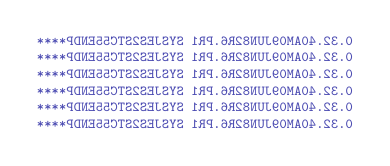
\begin{tikzpicture}
\node[xscale=-1,transform shape,align=left,text=blue!40!gray,font=\ttfamily\tiny] {
\unsure{0.32.40AM09JUN82R6.PR1 SYSJES2STC55ENDP****}\\
\unsure{0.32.40AM09JUN82R6.PR1 SYSJES2STC55ENDP****}\\
\unsure{0.32.40AM09JUN82R6.PR1 SYSJES2STC55ENDP****}\\
\unsure{0.32.40AM09JUN82R6.PR1 SYSJES2STC55ENDP****}\\
\unsure{0.32.40AM09JUN82R6.PR1 SYSJES2STC55ENDP****}\\
\unsure{0.32.40AM09JUN82R6.PR1 SYSJES2STC55ENDP****}
};
\end{tikzpicture}}

\diagram{\begin{tikzcd}
0\arrow[r]&V(J)\arrow[r]&\unsure{\mathfrak S_I}\arrow[r]&\unsure{\mathfrak S_J}\arrow[r]&1
\end{tikzcd}}

\figure{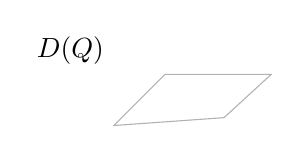
\begin{tikzpicture}[scale=1]
\node[above left] at (0,0.65) {$\unsure{D(Q)}$};
\draw[gray!60] (0,0)--(.65,.65)--(2,.65)--(1.4,.1)--cycle;
\end{tikzpicture}}

\[
\boxed{\left\{\begin{aligned}
\rho^3&=\sigma^2=1\\
\rho\sigma&=\ell
\end{aligned}\right.}
\]

\diagram{\begin{tikzcd}[column sep=small,row sep=large]
1\arrow[r]&
\unsure{\Gamma|\mathcal T}_{0,4}^{!}\arrow[r]\arrow[d,"\simeq",draw=none]&
\unsure{\Gamma|\mathcal T}_{04}^{\deleted{\unsure{!}}}\arrow[r]\arrow[d]&
\unsure{\mathfrak S_4}\arrow[r]\arrow[d]&1\\
1\arrow[r]&
\Pi_{0,3}\arrow[r,very thick]\arrow[d,"\simeq",draw=none]&
\unsure{\Gamma|\mathcal T}_{04}'\arrow[r]&
\unsure{\mathfrak S_3}\arrow[r,dash]&1\\
1\arrow[r]&
\Pi_{0,\unsure{3|5}}^{\unsure{2}}\arrow[r,very thick]&
\unsure{\Gamma|\mathcal T}_{1,1}\arrow[r]\arrow[u]&
\unsure{\widetilde{\mathfrak S}_3}\arrow[u]
\end{tikzcd}}

\margin{cart}

\[
\begin{aligned}
\unsure{\mathfrak S_4}&\simeq\operatorname{Aff}(2,\mathbb Z/2\mathbb Z)\\
\unsure{\mathfrak S_3}&\quad\text{``}\operatorname{Sl}(2,\mathbb Z/2\mathbb Z)\\
\unsure{\widetilde{\mathfrak S}_3}&\simeq\operatorname{Sl}(2,\mathbb Z/4\mathbb Z)/-\\
\unsure{\Gamma|\mathcal T}_{1,1}&\simeq\operatorname{Sl}(2,\mathbb Z)
\end{aligned}
\]

\margin{19}
\scanpage{21}

\figure{\begin{tikzpicture}[scale=.9]
\draw (-4.5,4.5)..controls(-4.2,4.65)and(-4,4.6)..(-3.8,4.45);
\draw[gray!65] (0.1,2.1)..controls(-.05,2.4)and(.02,5.1)..(.12,5.1)..controls(.24,5.1)and(.27,2.2)..(.1,2.1);
\draw[gray!65] (-3.6,3.5)--(-1.4,1.1);
\draw[gray!65] (-3.9,-1.5)--(-1.9,0);
\draw[gray!65] (-.25,-.8)--(-.3,-3.4);
\draw[gray!65] (.65,-.15)..controls(1.5,-.7)..(2.6,-1.7);
\draw[gray!65] (2.25,2.2)--(3.8,3.8);
\draw[thick] (-1.15,.2)--(-.15,1.55)--(.7,.55)--(.18,-.3)--cycle;
\draw[thick] (-.15,1.55)--(.18,-.3);
\draw[dashed] (-1.15,.2)--(.7,.55);
\draw[gray] (1.4,1.2)--(2.15,2.4)--(3.05,1.75)--(2.55,.95)--cycle;
\draw[gray] (2.15,2.4)--(2.55,.95) (1.4,1.2)--(3.05,1.75);
\draw[gray,thick] (1.35,.85)--(2.75,2.05);
\draw[dashed] (1.8,1.05)--(2.75,2.05);
\end{tikzpicture}}

\scalebox{-1}[1]{\diagram{\begin{array}{ll}
\unsure{\mathtt{\phantom{G}GGGGGGGGGG\phantom{G}}}&\unsure{\mathtt{UU\phantom{UUUUUUUU}UU}}\\
\unsure{\mathtt{GGGGGGGGGGGG}}&\unsure{\mathtt{UU\phantom{UUUUUUUU}UU}}\\
\unsure{\mathtt{GG\phantom{GGGGGGGG}GG}}&\unsure{\mathtt{UU\phantom{UUUUUUUU}UU}}\\
\unsure{\mathtt{GG\phantom{GGGGGGGGGG}}}&\unsure{\mathtt{UU\phantom{UUUUUUUU}UU}}\\
\unsure{\mathtt{GG\phantom{GGGGGGGGGG}}}&\unsure{\mathtt{UU\phantom{UUUUUUUU}UU}}\\
\unsure{\mathtt{GG\phantom{GGGGGGGGGG}}}&\unsure{\mathtt{UU\phantom{UUUUUUUU}UU}}\\
\unsure{\mathtt{GG\phantom{GGGGG}GGGGG}}&\unsure{\mathtt{UU\phantom{UUUUUUUU}UU}}\\
\unsure{\mathtt{GG\phantom{GGGGG}GGGGG}}&\unsure{\mathtt{UU\phantom{UUUUUUUU}UU}}\\
\unsure{\mathtt{GG\phantom{GGGGGGGG}GG}}&\unsure{\mathtt{UU\phantom{UUUUUUUU}UU}}\\
\unsure{\mathtt{GG\phantom{GGGGGGGG}GG}}&\unsure{\mathtt{UU\phantom{UUUUUUUU}UU}}\\
\unsure{\mathtt{GGGGGGGGGGGG}}&\unsure{\mathtt{UUUUUUUUUUUU}}\\
\unsure{\mathtt{\phantom{G}GGGGGGGGGG\phantom{G}}}&\unsure{\mathtt{\phantom{U}UUUUUUUUUU\phantom{U}}}
\end{array}}}

\scalebox{-1}[1]{\diagram{\begin{array}{llllll}
\unsure{\mathtt{****P}}&\unsure{\mathtt{END}}&\unsure{\mathtt{STC}}&\unsure{\mathtt{55|35}}&\unsure{\mathtt{GUTS}}&\unsure{\mathtt{ROOM}}\\
\unsure{\mathtt{****P}}&\unsure{\mathtt{END}}&\unsure{\mathtt{STC}}&\unsure{\mathtt{55|35}}&\unsure{\mathtt{GUTS}}&\unsure{\mathtt{ROOM}}\\
\unsure{\mathtt{****P}}&\unsure{\mathtt{END}}&\unsure{\mathtt{STC}}&\unsure{\mathtt{55|35}}&\unsure{\mathtt{GUTS}}&\unsure{\mathtt{ROOM}}\\
\unsure{\mathtt{****P}}&\unsure{\mathtt{END}}&\unsure{\mathtt{STC}}&\unsure{\mathtt{55|35}}&\unsure{\mathtt{GUTS}}&\unsure{\mathtt{ROOM}}\\
\unsure{\mathtt{****P}}&\unsure{\mathtt{END}}&\unsure{\mathtt{STC}}&\unsure{\mathtt{55|35}}&\unsure{\mathtt{GUTS}}&\unsure{\mathtt{ROOM}}\\
\unsure{\mathtt{****P}}&\unsure{\mathtt{END}}&\unsure{\mathtt{STC}}&\unsure{\mathtt{55|35}}&\unsure{\mathtt{GUTS}}&\unsure{\mathtt{ROOM}}
\end{array}}}

\margin{20}
\scanpage{22}

\texttt{//* GUTS 0055 I}

\[
\boxed{5400-5420}
\]

\margin{(93) 51, 81, 00 \quad \unsure{411}}

\diagram{\begin{array}{ll}
\left[
\begin{array}{ll}
\left\{\begin{array}{l}
-\ \text{Mr BEZOT}\\
\text{lab \unsure{cl.|ch.} des liquides}\\
\text{parc Valrose}\\
\text{\unsure{06034|06024} Nice}
\end{array}\right.
&
\begin{array}{l}
-\ \text{soumission}\\
-\ \text{récupération}\\
\text{T.S.O.}
\end{array}
\end{array}
\right]
&
-\ \left\{\begin{array}{l}
\text{NPL PLN1A}\\
\text{BEZOT}
\end{array}\right.
\end{array}}

\diagram{\begin{array}{llll}
\mathtt{\phantom{G}GGGGGGGGGG\phantom{G}}&
\mathtt{UU\phantom{UUUUUUUU}UU}&
\mathtt{TTTTTTTTTTTT}&
\mathtt{\phantom{S}SSSSSSSSSS\phantom{S}}\\
\mathtt{GGGGGGGGGGGG}&
\mathtt{UU\phantom{UUUUUUUU}UU}&
\mathtt{TTTTTTTTTTTT}&
\mathtt{SSSSSSSSSSSS}\\
\mathtt{GG\phantom{GGGGGGGG}GG}&
\mathtt{UU\phantom{UUUUUUUU}UU}&
\mathtt{\phantom{TTTTT}TT\phantom{TTTTT}}&
\mathtt{SS\phantom{SSSSSSSS}SS}\\
\mathtt{GG\phantom{GGGGGGGGGG}}&
\mathtt{UU\phantom{UUUUUUUU}UU}&
\mathtt{\phantom{TTTTT}TT\phantom{TTTTT}}&
\mathtt{SS\phantom{SSSSSSSSSS}}\\
\mathtt{GG\phantom{GGGGGGGGGG}}&
\mathtt{UU\phantom{UUUUUUUU}UU}&
\mathtt{\phantom{TTTTT}TT\phantom{TTTTT}}&
\mathtt{SSS\phantom{SSSSSSSSS}}\\
\mathtt{GG\phantom{GGGGGGGGGG}}&
\mathtt{UU\phantom{UUUUUUUU}UU}&
\mathtt{\phantom{TTTTT}TT\phantom{TTTTT}}&
\mathtt{\phantom{S}SSSSSSSSS\phantom{SS}}\\
\mathtt{GG\phantom{GGGGG}GGGGG}&
\mathtt{UU\phantom{UUUUUUUU}UU}&
\mathtt{\phantom{TTTTT}TT\phantom{TTTTT}}&
\mathtt{\phantom{SS}SSSSSSSSS\phantom{S}}\\
\mathtt{GG\phantom{GGGGG}GGGGG}&
\mathtt{UU\phantom{UUUUUUUU}UU}&
\mathtt{\phantom{TTTTT}TT\phantom{TTTTT}}&
\mathtt{\phantom{SSSSSSSSS}SSS}\\
\mathtt{GG\phantom{GGGGGGGG}GG}&
\mathtt{UU\phantom{UUUUUUUU}UU}&
\mathtt{\phantom{TTTTT}TT\phantom{TTTTT}}&
\mathtt{\phantom{SSSSSSSSSS}SS}\\
\mathtt{GG\phantom{GGGGGGGG}GG}&
\mathtt{UU\phantom{UUUUUUUU}UU}&
\mathtt{\phantom{TTTTT}TT\phantom{TTTTT}}&
\mathtt{SS\phantom{SSSSSSSS}SS}\\
\mathtt{GGGGGGGGGGGG}&
\mathtt{UUUUUUUUUUUU}&
\mathtt{\phantom{TTTTT}TT\phantom{TTTTT}}&
\mathtt{SSSSSSSSSSSS}\\
\mathtt{\phantom{G}GGGGGGGGGG\phantom{G}}&
\mathtt{\phantom{U}UUUUUUUUUU\phantom{U}}&
\mathtt{\phantom{TTTTT}TT\phantom{TTTTT}}&
\mathtt{\phantom{S}SSSSSSSSSS\phantom{S}}
\end{array}}

\begin{tabular}{l}
\texttt{****P END STC 55 GUTS}\quad\texttt{ROOM}\quad\texttt{10.32.40 AM 09 JUN 82 R6.PR1}\quad\texttt{SYS JES2 STC 55 END P****}\\
\texttt{****P END STC 55 GUTS}\quad\texttt{ROOM}\quad\texttt{10.32.40 AM 09 JUN 82 R6.PR1}\quad\texttt{SYS JES2 STC 55 END P****}\\
\texttt{****P END STC 55 GUTS}\quad\texttt{ROOM}\quad\texttt{10.32.40 AM 09 JUN 82 R6.PR1}\quad\texttt{SYS JES2 STC 55 END P****}\\
\texttt{****P END STC 55 GUTS}\quad\texttt{ROOM}\quad\texttt{10.32.40 AM 09 JUN 82 R6.PR1}\quad\texttt{SYS JES2 STC 55 END P****}\\
\texttt{****P END STC 55 GUTS}\quad\texttt{ROOM}\quad\texttt{10.32.40 AM 09 JUN 82 R6.PR1}\quad\texttt{SYS JES2 STC 55 END P****}\\
\texttt{****P END STC 55 GUTS}\quad\texttt{ROOM}\quad\texttt{10.32.40 AM 09 JUN 82 R6.PR1}\quad\texttt{SYS JES2 STC 55 END P****}
\end{tabular}

\margin{21}
\scanpage{23}

\begin{flushright}
\texttt{AVANCE SUR PROGRAMMATION AU 26/0}
\end{flushright}

\texttt{MAIN-D'OEUVRE NECESSAIRES A LA FABRICATION DE 1 S}

\begin{tabular}{lll}
002&TRONCONNAGE ALU&0,18 HEURES\\
004&POINCONNAGE ALU&0,18 HEURES\\
013&SOUDURE SKYDOME&0,34 HEURES\\
020&EBARBAGE&0,20 HEURES\\
021&PLAQUES&0,16 HEURES\\
025&COLLAGE&0,42 \unsure{HEURES}\\
026&MONTAGE SKYDOME&1,0\unsure{8} \unsure{HEURES}
\end{tabular}

\texttt{CHARGE GLOBALE MAIN-D OEUVRE POUR \unsure{LA FABRICATION} DE}

\texttt{COUT PRODUCTION \quad \unsure{418,60|418.60} FRS \quad \unsure{PRIX DE CES}}

\figure{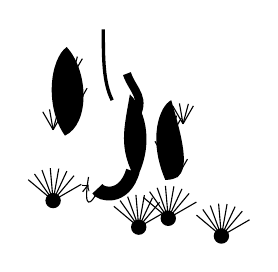
\begin{tikzpicture}[scale=.75]
\fill (0,1.1)..controls(-.35,1.6)and(-.25,2.4)..(.03,2.6)..controls(.4,2.2)and(.43,1.3)..(0,1.1);
\fill (1.2,.35)..controls(.9,.9)and(1,1.2)..(1.1,1.8)..controls(1.4,1.5)and(1.5,.9)..(1.2,.35);
\draw[very thick] (.8,1.7)..controls(.65,2)and(.65,2.4)..(.65,2.9);
\draw[line width=3pt] (1.16,1.35)..controls(1.4,1.75)and(1.15,1.85)..(1.05,2.15);
\draw[line width=5pt] (1.15,.5)..controls(1,0)and(.6,.1)..(.55,.2);
\fill (1.7,.35)..controls(1.4,1.05)and(1.6,1.6)..(1.8,1.7)..controls(2.1,.7)and(2.1,.35)..(1.7,.35);
\foreach \x/\y in {-.2/1.2,0/1.7,.12/2.1,.2/1.6,1.7/.7,1.8/1.1,1.9/.4,2/1.3}{
\foreach \a in {60,75,100,120}{\draw[thin] (\x,\y)--++(\a:.35);}}
\foreach \x/\y in {-.2/0,1.25/-.45,1.75/-.3,2.65/-.6}{
\fill (\x,\y) ellipse (.13 and .13);
\foreach \a in {30,50,65,80,95,110,125,140}{\draw (\x,\y)--++(\a:.55);}}
\draw (.4,.4)..controls(.3,-.2)and(.45,-.05)..(.55,.15);
\draw[->] (.3,.15)--(.4,.27);
\end{tikzpicture}}

\figure{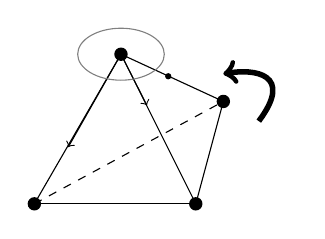
\begin{tikzpicture}[scale=1]
\coordinate (A) at (0,0); \coordinate (B) at (1.1,1.9);
\coordinate (C) at (2.05,0); \coordinate (D) at (2.4,1.3);
\draw (A)--(B)--(C)--(D)--(B);
\draw[thin] (A)--(C);
\draw[dashed] (A)--(D);
\foreach \p in {A,B,C,D}{\fill (\p) circle (.085);}
\draw[->] (B)--(.43,.72);
\draw[->] (B)--(1.43,1.25);
\fill (1.7,1.62) circle (.04);
\draw[gray] (B) ellipse (.55 and .33);
\draw[line width=2pt,->] (2.85,1.05)..controls(3.3,1.65)and(2.8,1.72)..(2.4,1.65);
\end{tikzpicture}}

\diagram{\begin{tikzcd}[column sep=small]
\left.\begin{array}{l}\deleted{\unsure{4|6}\text{ hexagones}}\\\deleted{4\text{ sommets}}\end{array}\right\}
\arrow[r,bend left]
&
\begin{array}{l}
8\text{ triangles}\\
4\text{ sommets d'ordre }6\\
12\text{ arêtes}
\end{array}
\end{tikzcd}}

\[
\unsure{A_4|\mathfrak S_4}
\]

\[
\deleted{\unsure{\widetilde{\mathfrak S}_3}}:
\qquad \unsure{\mu_6|\mathbb H_6}\times(\mathbb Z/2\mathbb Z)^2
\]
\[
\unsure{\mu_4|\mathbb H_4}\times(\mathbb Z/2\mathbb Z)^2
\]

\uline{Hexagone}

\uline{orienté}

\figure{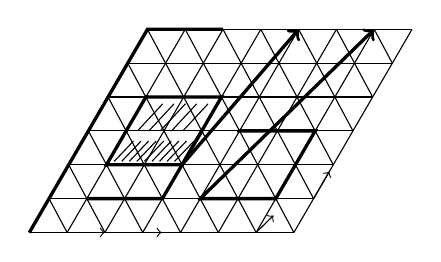
\begin{tikzpicture}[x={(.48cm,0cm)},y={(.25cm,.43cm)}]
\foreach \y in {0,...,6}{\draw (0,\y)--(7,\y);}
\foreach \x in {0,...,7}{\draw (\x,0)--(\x,6);}
\foreach \s in {1,...,12}{
\draw ({max(0,\s-6)},{min(6,\s)})--({min(7,\s)},{max(0,\s-7)});
}
\draw[very thick] (0,0)--(0,6)--(2,6);
\draw[very thick] (1,2)--(1,4)--(3,4)--(3,2)--cycle;
\draw[very thick,->] (3,2)--(4,6);
\draw[very thick,->] (4,1)--(6,6);
\draw[very thick] (4,1)--(6,1)--(6,3)--(4,3);
\draw[very thick] (1,1)--(3,1)--(3,3);
\foreach \x in {1.15,1.35,1.55,1.75,1.95,2.15,2.35,2.55,2.75}{\draw[thin] (\x,2.1)--(\x+.2,2.7);}
\foreach \x in {1.3,1.6,1.9,2.2,2.5}{\draw[thin] (\x,3)--(\x+.25,3.8);}
\draw[->] (1,0)--(2,0); \draw[->] (3,0)--(3.5,0);
\draw[->] (6,0)--(6.2,.5); \draw[->] (7,1)--(7,1.8);
\foreach \p in {(1,2),(1,4),(3,4),(3,2),(4,1),(6,1),(6,3),(4,3)}{\fill \p circle (.06);}
\end{tikzpicture}}

\margin{trois arêtes\\trois sommets}

\uline{Carré orienté}

\figure{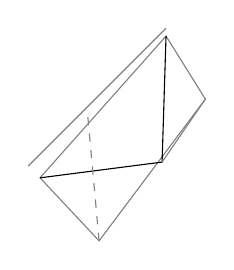
\begin{tikzpicture}[scale=1]
\draw[gray] (0,0)--(1.6,1.8)--(2.1,1)--(.75,-.8)--cycle;
\draw (0,0)--(1.55,.2)--(1.6,1.8);
\draw[gray] (1.55,.2)--(2.1,1);
\draw[dashed,gray] (.75,-.8)--(.6,.85);
\draw[gray] (-.15,.15)--(1.6,1.9);
\end{tikzpicture}}

\figure{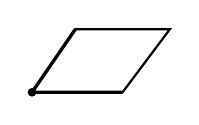
\begin{tikzpicture}[scale=1]
\draw[thick] (0,0)--(.55,.8)--(1.75,.8)--(1.15,0)--cycle;
\draw[very thick] (0,0)--(.55,.8) (0,0)--(1.15,0);
\fill (0,0) circle (.055);
\end{tikzpicture}}

\figure{\begin{tikzpicture}[scale=.8]
\draw[->] (0,1.3)--(0,0);
\draw[gray] (0,1.3)--(1.2,1.3)--(1.2,0);
\draw[gray] (0,1.3)--(.25,1.02);
\end{tikzpicture}}

\figure{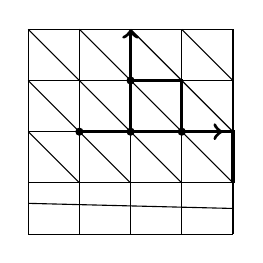
\begin{tikzpicture}[scale=.65]
\foreach \x in {0,1,2,3,4}{\draw (\x,0)--(\x,4);}
\foreach \y in {0,1,2,3,4}{\draw (0,\y)--(4,\y);}
\foreach \x in {0,1,2,3}{\foreach \y in {1,2,3}{\draw (\x,\y+1)--(\x+1,\y);}}
\draw[very thick,->] (2,2)--(2,4);
\draw[very thick,->] (1,2)--(3.8,2);
\draw[very thick] (2,3)--(3,3)--(3,2)--(4,2)--(4,1);
\foreach \p in {(1,2),(2,2),(2,3),(3,2)}{\fill \p circle (.08);}
\draw (0,.6)--(4,.5);
\end{tikzpicture}}

\figure{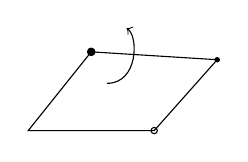
\begin{tikzpicture}[scale=1]
\draw (0,0)--(.8,1)--(2.4,.9)--(1.6,0)--cycle;
\fill (.8,1) circle (.055); \fill (2.4,.9) circle (.035);
\draw (1.6,0) circle (.04);
\draw[->] (1,.6)..controls(1.4,.6)and(1.4,1.2)..(1.25,1.3);
\end{tikzpicture}}

$4$ carrés

$8$ arêtes

$4$ sommets

\fbox{\diagram{\begin{tikzcd}
E_{\varepsilon+}\arrow[r,bend left,very thick]\arrow[d,leftrightarrow,very thick]&
E_{\varepsilon,-}\arrow[l,bend left,very thick]\arrow[d,leftrightarrow,very thick]\\
\overline E_Q\arrow[r,very thick]&\overline E_H
\end{tikzcd}}}

\margin{22}
\scanpage{24}
\margin{Mireille \& enfants}
\figure{
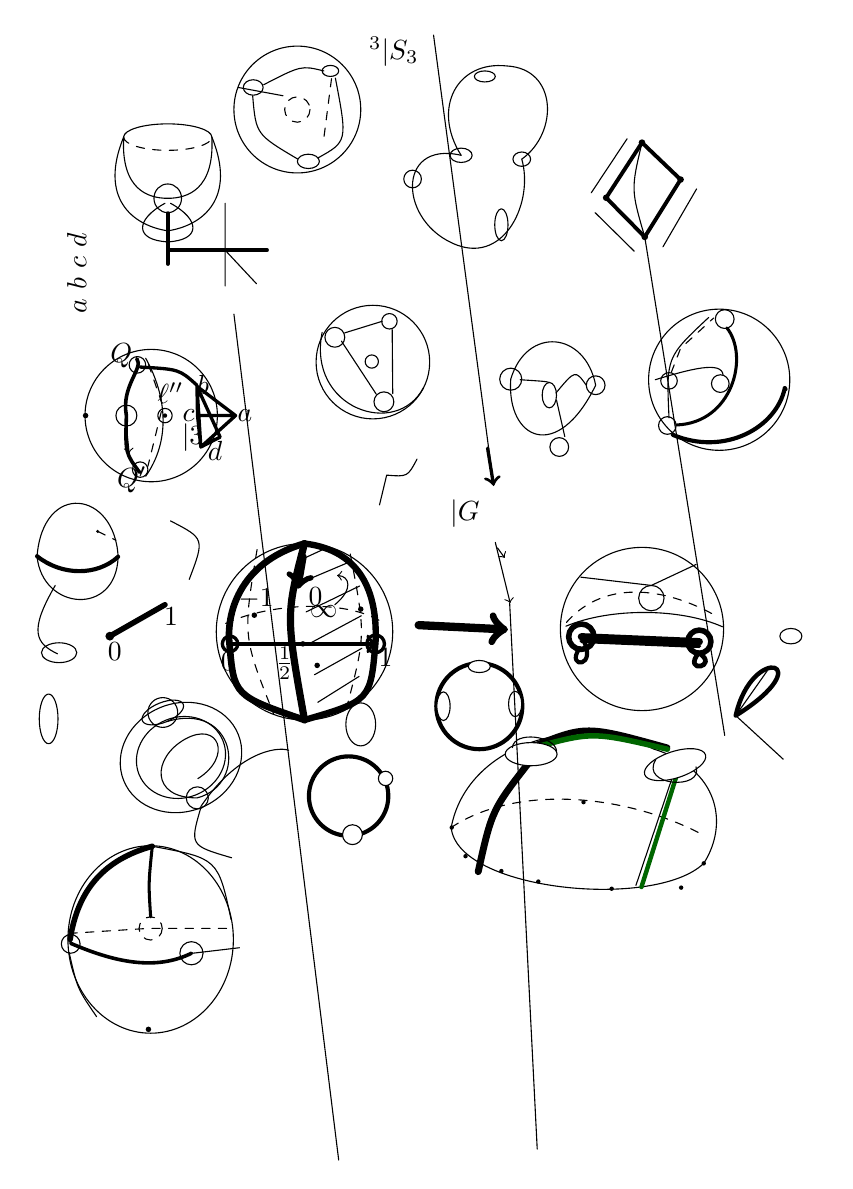
\begin{tikzpicture}[x=.007cm,y=-.007cm,line cap=round,line join=round]
\begin{scope}[shift={(330,425)}]
\draw (-80,-80) arc[start angle=180,end angle=360,x radius=80,y radius=24];
\draw[dashed] (-80,-80) arc[start angle=180,end angle=0,x radius=80,y radius=24];
\draw (-80,-80) .. controls (-125,30) and (-65,80) .. (0,90) .. controls (65,80) and (125,30) .. (80,-80);
\draw (-80,-80) .. controls (-85,15) and (-36,31) .. (0,31) .. controls (36,31) and (85,15) .. (80,-80);
\draw (0,31) ellipse (25 and 26);
\draw (-5,40) .. controls (-60,70) and (-60,107) .. (0,110) .. controls (60,107) and (60,70) .. (5,40);
\draw[line width=1.4pt] (0,58)--(0,125)--(180,125) (0,98)--(0,150);
\draw (104,40)--(104,190) (104,125)--(161,186);
\end{scope}
\begin{scope}[shift={(565,295)}]
\draw (0,0) circle (115);
\draw (-80,-40) ellipse (18 and 14) (20,94) ellipse (20 and 13) (60,-70) ellipse (15 and 10);
\draw (-81,-25) .. controls (-75,45) .. (1,90) (37,88) .. controls (91,58) .. (69,-57);
\draw (-61,-45) .. controls (7,-80) .. (48,-70);
\draw[dashed] (62,-56)--(47,60) (0,0) circle (23);
\draw (-107,-40)--(-26,-25);
\end{scope}
\node at (740,190) {\(\unsure{\circlearrowleft^{3}|\mathfrak S_3}\)};
\begin{scope}[shift={(900,380)}]
\draw (-38,-2) .. controls (-92,-88) and (-45,-174) .. (45,-164) .. controls (137,-159) and (139,-43) .. (72,5);
\draw (-38,-2) ellipse (20 and 13) (72,5) ellipse (16 and 13) (5,-145) ellipse (19 and 10);
\draw (-38,-2) .. controls (-157,-30) and (-152,121) .. (-45,161) .. controls (42,193) and (94,82) .. (72,5);
\draw (-126,41) circle (16);
\draw (35,124) ellipse (12 and 29);
\end{scope}
\draw (812,160)--(921,977);
\draw[->,line width=1.2pt] (910,909)--(921,977);
\node at (869,1028) {\(\unsure{\circlearrowleft|G}\)};
\draw[->] (924,1080)--(951,1190);
\draw[->] (928,1090)--(941,1108);
\draw (450,666)--(640,2200);
\draw (714,1012)--(727,958) .. controls (765,961) .. (782,929);
\draw (335,1041) .. controls (397,1073) .. (369,1147);
\begin{scope}[shift={(1190,440)}]
\draw[line width=1.4pt] (0,-85)--(-65,15)--(5,86)--(70,-18)--cycle;
\draw (0,-85) .. controls (-20,0) .. (5,86);
\foreach \x/\y in {0/-85,-65/15,5/86,70/-18}{\fill (\x,\y) circle (6);}
\draw (-92,6)--(-27,-92) (-85,42)--(-14,112) (38,104)--(99,-1);
\end{scope}
\draw (1195,526)--(1340,1430);
\begin{scope}[shift={(300,850)},rotate=-90]
\draw (0,0) circle (120);
\draw[line width=1.3pt] (-103,26) .. controls (-86,13) and (-54,55) .. (0,45) .. controls (68,47) .. (103,21);
\draw (-104,10) .. controls (-34,-29) and (46,-35) .. (110,10);
\draw[dashed] (-93,5)--(-18,-21)--(92,6);
\draw (-92,25) circle (15) (98,20) circle (14) (0,-25) circle (13);
\draw (0,45) circle (19);
\fill (0,-25) circle (4);
\fill (0,119) circle (5);
\draw[line width=1.2pt] (-88,20) .. controls (-84,-51) .. (-55,-83);
\draw[line width=1.2pt] (-53,-83)--(0,-153)--(57,-90)--(-53,-83)--(0,-84)--(0,-153) (-53,-83)--(39,-125)--(57,-90) (0,-84)--(57,-90);
\node at (0,-170) {\(a\)};
\node at (-55,-94) {\(\unsure{b}\)};
\node at (0,-68) {\(\unsure{c}\)};
\node at (64,-116) {\(\unsure{d}\)};
\node at (40,-75) {\(\unsure{\circlearrowleft|3}\)};
\node at (-40,-35) {\(\ell''\)};
\node at (-108,54) {\(Q\)};
\node at (117,35) {\(Q'\)};
\draw[->] (18,45)--(68,40);
\end{scope}
\node[rotate=90] at (165,592) {\(a\ b\ c\ d\)};
\begin{scope}[shift={(702,753)}]
\draw (0,0) circle (103);
\draw (-69,-45) circle (18) (30,-74) circle (14) (20,72) circle (18) (-2,-1) circle (12);
\draw (-57,-38)--(6,58) (36,57)--(35,-60) (17,-74)--(-51,-53);
\draw (-92,-54) .. controls (-120,84) and (43,140) .. (92,46);
\end{scope}
\begin{scope}[shift={(1030,802)}]
\draw (-78,-18) .. controls (-86,91) and (6,136) .. (76,-7) .. controls (57,-105) and (-49,-115) .. (-78,-18);
\draw (-78,-18) circle (20) (76,-7) circle (17) (10,105) circle (17);
\draw (-8,11) ellipse (13 and 23);
\draw (-61,-17) .. controls (-15,-14) .. (-8,-12) (5,20)--(20,86) (4,7) .. controls (39,-35) .. (59,-7);
\end{scope}
\begin{scope}[shift={(1330,785)}]
\draw (0,0) circle (128);
\draw (-94,83) circle (16) (2,7) circle (16) (10,-110) circle (17) (-91,2) circle (15);
\draw[line width=1.1pt] (-77,82) .. controls (24,78) and (55,-42) .. (14,-94);
\draw[line width=1.5pt] (-84,100) .. controls (10,139) and (104,87) .. (119,15);
\draw (-91,69) .. controls (-96,-41) .. (-19,-113);
\draw[dashed] (-87,-13)--(-70,-57)--(-10,-112);
\draw (-116,0) .. controls (-50,-20) and (4,-34) .. (7,-9);
\fill (120,17) circle (4);
\end{scope}
\begin{scope}[shift={(168,1110)}]
\draw (-75,-5) .. controls (-64,-142) and (66,-124) .. (72,-4) .. controls (69,105) and (-66,94) .. (-75,-5);
\draw[line width=1.5pt] (-75,-5) .. controls (-30,31) and (34,31) .. (72,-4);
\fill (35,-50) circle (3);
\draw[dashed] (35,-50)--(68,-34);
\draw (-42,48) .. controls (-91,132) and (-77,153) .. (-38,172);
\draw (-35,170) ellipse (32 and 18);
\end{scope}
\draw[line width=2pt] (225,1250)--(325,1193);
\fill (225,1250) circle (8);
\node at (234,1278) {\(0\)};
\node at (336,1214) {\(1\)};
\draw (114,1400) ellipse (17 and 45);
\begin{scope}[shift={(578,1242)}]
\draw (0,0) circle (160);
\draw[line width=2.4pt] (0,-160) .. controls (-121,-125) and (-142,-29) .. (-136,22) .. controls (-128,116) .. (0,160);
\draw[line width=2.3pt] (0,-160) .. controls (102,-148) and (132,-71) .. (129,16) .. controls (120,125) .. (0,160);
\draw[line width=2.6pt] (0,-160) .. controls (-34,-30) .. (0,160);
\draw[->,line width=2.4pt] (-2,-136)--(-12,-78);
\draw[->,line width=1.4pt] (-138,22)--(131,22);
\draw[dashed] (-143,-15) .. controls (-71,-49) and (72,-63) .. (143,-16);
\draw[dashed] (-86,-149) .. controls (-112,8) .. (-56,149) (83,-141) .. controls (111,6) .. (76,139);
\foreach \x/\y in {-135/22,-3/22,129/22,-91/-30,102/-41,23/61,0/156}{\fill (\x,\y) circle (5);}
\draw[line width=1.2pt] (-135,22) circle (14) (129,22) circle (16);
\foreach \a/\b/\c/\d in {3/-135/42/-153,0/-92/78/-125,3/-36/100/-83,8/22/103/-29,18/78/104/30,24/128/99/81}{\draw (\a,\b)--(\c,\d);}
\draw[->] (55,-49) .. controls (89,-77) and (82,-101) .. (59,-102);
\node at (-88,-60) {\(-1\)};
\node at (-36,57) {\(\frac12\)};
\node at (20,-64) {\(\unsure{0}\)};
\node at (35,-37) {\(\unsure{\infty}\)};
\node at (-139,55) {\(\unsure{0}\)};
\node at (147,46) {\(\unsure{1}\)};
\end{scope}
\draw[->,line width=3pt] (785,1230)--(947,1238);
\begin{scope}[shift={(1190,1237)}]
\draw (0,0) circle (148);
\draw (-138,-5) .. controls (-57,-39) and (70,-38) .. (146,-4);
\draw[dashed] (-137,-12) .. controls (-64,-95) and (52,-72) .. (139,-21);
\draw[line width=1.4pt] (-110,22)--(104,31);
\draw[line width=2.6pt] (-110,14)--(104,23);
\draw[line width=2pt] (-110,14) circle (23) (104,23) circle (21);
\draw (17,-56) circle (23);
\draw (-111,-94)--(17,-79)--(98,-117);
\draw[line width=1.5pt] (-113,35) .. controls (-141,73) and (-75,72) .. (-110,14);
\draw[line width=1.7pt] (103,43) .. controls (72,82) and (142,69) .. (103,43);
\end{scope}
\draw (1460,1250) ellipse (20 and 14);
\draw[line width=1.6pt] (1360,1394) .. controls (1390,1261) and (1517,1296) .. (1360,1394);
\draw (1360,1394)--(1446,1473) (1360,1394)--(1417,1313);
\draw (680,1410) ellipse (27 and 39);
\begin{scope}[shift={(895,1377)}]
\draw[line width=1.5pt] (0,0) circle (78);
\draw[fill=white] (-65,0) ellipse (12 and 26) (65,-4) ellipse (12 and 23) (0,-72) ellipse (20 and 11);
\end{scope}
\begin{scope}[shift={(354,1470)},rotate=22]
\draw (0,0) ellipse (112 and 98);
\draw (0,0) ellipse (82 and 73);
\draw (0,-88) ellipse (40 and 18);
\draw (0,-88) circle (27);
\draw (0,79) circle (20);
\draw (0,-70) .. controls (130,-59) and (97,91) .. (0,79) .. controls (-79,48) and (-49,-19) .. (19,-28) .. controls (89,-37) and (88,34) .. (14,47);
\draw (0,97) .. controls (-45,154) .. (17,203);
\draw (0,96) .. controls (96,31) and (167,45) .. (186,61);
\end{scope}
\begin{scope}[shift={(658,1540)}]
\draw[line width=1.5pt] (0,0) circle (72);
\draw[fill=white] (7,70) circle (18) (67,-32) circle (13);
\draw[dashed] (-66,-32)--(-44,-59);
\end{scope}
\begin{scope}[shift={(299,1800)}]
\draw (0,0) ellipse (150 and 170);
\draw[line width=2pt] (-146,0) .. controls (-130,-105) and (-69,-149) .. (3,-169);
\draw (3,-169) .. controls (122,-147) .. (146,-36);
\draw[line width=1.3pt] (-145,7) .. controls (-68,40) and (7,58) .. (74,25);
\draw (76,25)--(161,15);
\draw[dashed] (-148,-11)--(-5,-20)--(139,-20);
\draw (-145,8) circle (17) (74,25) circle (21);
\draw[dashed] (0,-20) circle (21);
\draw[line width=1.1pt] (3,-169) .. controls (-4,-102) .. (0,-41);
\draw (-148,23) .. controls (-133,89) .. (-98,140);
\fill (-4,163) circle (5);
\end{scope}
\begin{scope}[shift={(1080,1557)}]
\draw (-236,40) .. controls (-208,-108) and (-15,-171) .. (132,-102) .. controls (249,-66) and (268,33) .. (222,105);
\draw (-236,40) .. controls (-225,155) and (134,190) .. (222,105);
\draw[dashed] (-236,40) .. controls (-115,-40) and (83,-20) .. (222,54);
\draw[line width=2.5pt] (-187,120) .. controls (-162,8) .. (-91,-83);
\draw[line width=2.2pt] (-91,-106) .. controls (8,-146) .. (156,-105);
\draw[green!40!black,line width=2pt] (-89,-104) .. controls (20,-134) .. (156,-102);
\draw[green!40!black,line width=1.6pt] (174,-58)--(109,148);
\draw (164,-48)--(99,145);
\draw[fill=white] (-91,-93) ellipse (47 and 21);
\draw (-125,-105) .. controls (-122,-136) and (-47,-126) .. (-45,-99);
\draw[fill=white,rotate around={18:(170,-74)}] (170,-74) ellipse (58 and 24);
\draw (135,-83) .. controls (105,-35) and (222,-27) .. (208,-70);
\foreach \x/\y in {-235/40,-210/92,-145/119,-78/138,55/151,181/149,222/105,4/-6}{\fill (\x,\y) circle (4);}
\end{scope}
\draw (950,1190)--(1000,2180);
\end{tikzpicture}
}% crop-candidate: scan 24
\margin{\(\operatorname{diag}_Q\simeq\omega_Q\)\quad
\(\operatorname{diag}_Q\wedge\omega_Q\simeq\operatorname{codiag}_Q\)}
\margin{\unsure{avec} un ens à trois éléments, on fait \(3\times2=6\) courbes \unsure{elliptiques} de type \((1,1)\)}
avec un ens \(I\) de card \(4\),
\unsure{on} trouve \(\unsure{17|14}\) \unsure{points|ponts} \unsure{or|ou} canoniques \inserted{de type \((0,4)\)}
\((14=3\times4+\deleted{3\times}2)\)
dont deux tétraèdres,
\deleted{quatre}\inserted{trois} carrés, \deleted{deux} \(2\times3=6\)
assemblages de \deleted{\unsure{F}} ``T'' droits,
\(6=2\times3\) assemblages de \inserted{\(1\)} T gauches.
\margin{23}
\scanpage{25}
\diagram{\begin{array}{ll}
\unsure{A|\Delta}&\text{triangle}\\
\vec T&\text{tétraèdre orienté}\\
\overset{\deleted{\rightarrow}}{Q}&\text{carré }\deleted{\text{orienté}}\\
\unsure{\bar Q|\bar E}&\deleted{\text{hexagone}}\ \text{carré orienté}\\
\bar H&\text{hexagone orienté}
\end{array}}
\diagram{\begin{array}{c|c}
\begin{tikzcd}[row sep=small,column sep=large]
\Sigma_A & (0,3)\\
\Sigma_T \arrow[d,bend left=45,leftrightarrow] & (0,4)\\
\Sigma_Q & \\
E_{\vec Q} & \Bigg\}(1,1)\\
E_{\vec H} & \\
 & (0,5)\\
 & (1,2)
\end{tikzcd}
&
\begin{array}{l}
d=0\\[5pt]
\left.\begin{array}{c}d=1\\[9pt]\\[9pt]\\[9pt]\end{array}\right\}\\[10pt]
\left\{\begin{array}{c}\\[9pt]\end{array}\right. d=2
\end{array}
\end{array}}
\figure{\begin{tikzpicture}[x=.75cm,y=.75cm,line cap=round]
\draw (0,1.5)--(.45,1.54) (.85,1.55)--(1.2,1.59) (1.6,1.62)--(2.15,1.67) (2.55,1.71)--(3.1,1.73) (3.5,1.76)--(4.9,1.89);
\draw (.15,.42) .. controls (.36,.49) and (.48,.42) .. (.62,.45);
\draw (.85,.44) .. controls (1.4,.34) and (1.65,.65) .. (2.1,.58) .. controls (2.25,.57) and (2.4,.62) .. (2.7,.65)--(5.45,.96);
\draw (4.7,-2.1)--(4.94,-2.07);
\end{tikzpicture}}
\figure{\begin{tikzpicture}[x=.9cm,y=.9cm,line cap=round]
\draw (0,0)--(.8,2.1)--(2.1,1.1)--(1.4,-.9)--cycle;
\draw (.8,2.1)--(.53,3.5) (2.1,1.1)--(3.68,1.8) (1.4,-.9)--(1.79,-2.45) (0,0)--(-1.5,-.5);
\foreach \x/\y in {0/0,.8/2.1,2.1/1.1,1.4/-.9}{\fill (\x,\y) circle (2.4pt);}
\end{tikzpicture}}
\margin{24}
\scanpage{26}
\diagram{\begin{tikzcd}[column sep=large]
\begin{gathered}\text{Carte cellulaire (pas orientée) }\unsure{\text{conn}}\\
\text{dont tous les sommets sont}\\
\text{d'ordre }3\ \inserted{\text{ou }1}
\end{gathered}
\arrow[r,leftrightarrow] & \text{Cartes }\uline{\text{cellulaires}}
\end{tikzcd}}
\margin{\(\unsure{\mathrm{or}^{t}}\)}
triangulée \(\simeq\)
\margin{\(\deleted{\unsure{\mathbf Z}}\unsure{n-}\)}
revêtements de \(\mathbb P^1_{\unsure{\mathbb Q|\mathbb C}}\) ramifiés \unsure{seulement} en \(0,1,\infty\),
\figure{\begin{tikzpicture}[x=.0065cm,y=-.0065cm,line cap=round,line join=round]
\begin{scope}[shift={(1112,150)}]
\draw (0,-55) .. controls (-45,43) and (-13,83) .. (11,28) .. controls (29,-5) .. (0,-55);
\draw (0,-55) .. controls (-28,24) and (-17,67) .. (7,30) .. controls (15,0) .. (0,-55);
\draw (0,-51)--(-16,27)--(12,-12)--(-18,6) (0,-25)--(1,29);
\end{scope}
\begin{scope}[shift={(1340,170)}]
\draw (-110,101)--(0,-94)--(134,-62) (127,-52)--(83,91) (0,-94)..controls (18,-1)..(89,95) (-110,101)--(64,91);
\draw[line width=1.3pt] (-110,101)--(22,-12);
\draw (-119,111)--(17,-8)--(127,-52);
\end{scope}
\begin{scope}[shift={(1577,221)}]
\draw (0,0) ellipse (46 and 55);
\foreach \x/\y in {-6/-44,38/8,-31/48}{\draw (\x,\y) circle (15);\fill (\x,\y) circle (5);}
\end{scope}
\begin{scope}[shift={(300,680)}]
\draw[line width=1.5pt] (-104,-125) .. controls (-17,-98) and (4,-67) .. (80,-178);
\draw[line width=1.5pt] (165,-111) .. controls (74,-1) and (60,62) .. (94,151);
\draw[line width=1.5pt] (-134,-44) .. controls (-17,15) and (11,64) .. (18,179);
\draw (-139,-45) .. controls (-9,26) and (29,74) .. (18,179);
\draw (165,-111) .. controls (99,-28) and (69,29) .. (94,151);
\draw (-104,-125) .. controls (-147,-137) and (-169,-54) .. (-134,-44) .. controls (-106,-56) and (-94,-101) .. (-104,-125);
\draw (80,-178) .. controls (128,-189) and (184,-130) .. (165,-111) .. controls (124,-110) and (84,-146) .. (80,-178);
\draw (18,179) .. controls (28,136) and (74,126) .. (94,151) .. controls (74,177) and (34,186) .. (18,179);
\draw[->] (153,-120) .. controls (119,-132) .. (97,-164);
\draw[->] (-100,-117) .. controls (-109,-73) .. (-126,-55);
\draw[->] (24,172) .. controls (33,141) .. (78,144);
\foreach \x/\y in {-104/-125,-134/-44,80/-178,165/-111,18/179,94/151}{\fill (\x,\y) circle (5);}
\node at (-158,-105) {\(C\)};
\node at (174,-172) {\(B\)};
\node at (65,218) {\(A\)};
\node at (-91,-138) {\(c_B\)};
\node at (-135,-8) {\(c_A\)};
\node at (63,-195) {\(b_C\)};
\node at (194,-103) {\(b_A\)};
\node at (134,148) {\(a_B\)};
\node at (2,216) {\(a_C\)};
\node at (50,-47) {\(\unsure{\circlearrowleft|J}\)};
\end{scope}
\draw (529,370)--(700,553)--(639,759) (562,359)--(702,514) (527,394)--(659,550)--(612,739);
\draw (689,739)--(727,582)--(964,505) (700,553)--(961,459) (697,518)--(948,438);
\draw (498,645)--(788,356)--(849,681);
\draw (498,645) .. controls (658,640) and (748,707) .. (847,686);
\draw (870,690)--(1065,420);
\draw (1007,200)--(961,459)--(1113,582)--(1370,494);
\draw (1113,582) .. controls (1081,793) and (1037,863) .. (1054,1060);
\draw (431,950)--(626,771) .. controls (780,843) and (945,902) .. (1050,938)--(1333,896);
\draw[->] (1034,935)--(1080,936);
\draw[->] (1051,1030)--(1054,1060);
\foreach \x/\y in {961/459,1113/582,1370/494}{\fill (\x,\y) circle (5);}
\begin{scope}[shift={(1370,494)}]
\draw[line width=1.5pt] (0,0) .. controls (91,-197) and (266,-191) .. (232,-69) .. controls (216,33) and (115,46) .. (0,0);
\draw (0,0) .. controls (103,-191) and (229,-203) .. (226,-79) .. controls (231,19) and (78,52) .. (0,0);
\draw (0,0) .. controls (79,-198) and (253,-210) .. (241,-84) .. controls (232,40) and (78,42) .. (0,0);
\node at (187,-61) {\(\pm\)};
\end{scope}
\node at (1211,574) {\(\sigma_0\ \sigma_1\ \sigma_2\)};
\draw (1200,608)--(1200,615)--(1275,617)--(1275,608) (1294,612)--(1294,618)--(1353,620)--(1353,614);
\draw (945,684) .. controls (858,662) and (938,555) .. (1041,591) .. controls (1114,610) and (1153,663) .. (1079,673);
\draw[line width=2.2pt] (977,683)--(1071,671);
\fill (977,683) circle (8);
\node at (983,715) {\(0\)};
\node at (1073,700) {\(1\)};
\begin{scope}[shift={(1510,739)}]
\draw (-51,-105) .. controls (-6,-190) and (60,-192) .. (121,-136);
\draw (130,-26) .. controls (128,25) .. (111,80);
\draw (7,151) .. controls (-139,185) and (-119,53) .. (-116,7);
\draw (-74,-51) ellipse (49 and 64);
\draw (120,-79) ellipse (34 and 57);
\draw (64,122) ellipse (59 and 42);
\draw (-74,-113) .. controls (-156,-130) .. (-151,-43);
\draw (11,128) .. controls (10,81) .. (88,76);
\foreach \x/\y in {-51/-105,-116/7,121/-136,130/-26,111/80,7/151}{\fill (\x,\y) circle (3);}
\end{scope}
\draw (127,875) .. controls (77,786) and (226,757) .. (191,850) .. controls (173,879) .. (127,875)--(68,914) .. controls (102,988) and (19,959) .. (50,917);
\begin{scope}[shift={(287,1091)}]
\draw (0,0) ellipse (126 and 126);
\draw (0,0) ellipse (61 and 54);
\draw[line width=1.2pt] (0,-126) .. controls (-105,-97) and (-154,35) .. (-77,106) .. controls (0,152) .. (73,102);
\draw (0,-126) .. controls (-42,-113) and (-6,-9) .. (14,-102) .. controls (19,-126) .. (0,-126);
\fill (0,-126) circle (6);
\end{scope}
\begin{scope}[shift={(522,1113)}]
\draw[line width=1.2pt] (0,0) .. controls (61,-237) and (282,-129) .. (107,-43) .. controls (55,-17) .. (0,0) .. controls (-64,177) and (152,178) .. (0,0);
\fill (51,-24) circle (3);
\end{scope}
\draw (791,1105) .. controls (738,1062) and (903,1042) .. (926,1075);
\draw (947,1087) .. controls (998,1125) and (829,1160) .. (791,1105);
\foreach \x/\y in {878/1064,837/1127,925/1123}{\fill (\x,\y) circle (3);}
\draw (521,962)--(535,940);
\end{tikzpicture}}% crop-candidate: scan 26
\deleted{\unsure{cartes sphériques} \unsure{d}}
\[
\sigma_0^2=\sigma_1^2=\sigma_2^2=(\sigma_0\sigma_2)^2=(\sigma_0\sigma_1)^3=1
\]
\(\mathbb R\)-cartes \unsure{rigidifiées}
\margin{\(\sigma_0,\sigma_1,\sigma_2\)\quad \unsure{ses} pts fixes}
\margin{25}
\scanpage{27}
\figure{\begin{tikzpicture}[x=.009cm,y=-.009cm,line cap=round]
\draw (-140,-95) .. controls (-35,-143) and (46,-65) .. (62,18) .. controls (67,158) and (-27,220) .. (-78,233) .. controls (-198,204) and (-246,31) .. (-140,-95);
\draw (62,18) .. controls (127,-135) and (290,-143) .. (342,-44) .. controls (374,59) and (369,149) .. (286,190) .. controls (171,254) and (71,196) .. (51,119);
\draw (62,18) .. controls (8,69) and (8,129) .. (51,119);
\draw[dashed] (62,18) .. controls (87,89) .. (51,119);
\draw (-170,-68) .. controls (-106,-130) and (-103,-71) .. (-141,-60) .. controls (-184,-34) .. (-170,-68);
\draw (-171,171) .. controls (-112,147) and (-86,218) .. (-141,209);
\draw (270,-94) .. controls (250,-66) and (331,-19) .. (335,-47);
\draw[dashed] (270,-94)--(325,-65);
\draw (128,202) .. controls (150,222) and (224,227) .. (245,205);
\draw[dashed] (128,202) .. controls (173,178) .. (245,205);
\draw[gray!30] (-155,-13) .. controls (-31,5) and (-86,178) .. (-179,114);
\end{tikzpicture}}
\diagram{\begin{tikzcd}[column sep=large]
\left.\begin{array}{l}
4\text{ hexagones}\\16\ \unsure{\text{côtés}|\text{arêtes}}\\10\text{ sommets}
\end{array}\right\}
\arrow[r,Rightarrow] &
\begin{array}{l}8\text{ hexagones}\\\unsure{82|32}\text{ arêtes}\\16\text{ sommets}\end{array}
\\
\begin{array}{l}(\text{dont }4\text{ ramifiés})\\\text{d'ordre}\end{array}&
\end{tikzcd}}
\begin{gather*}
2\text{ hexag.}\\9\text{ arêtes}\\6\text{ sommets}
\end{gather*}
\figure{\begin{tikzpicture}[x=.0075cm,y=-.0075cm,line cap=round]
\draw[gray!30] (320,-440) ellipse (160 and 173);
\draw[gray!30] (178,-520)--(405,-582)--(474,-370)--(222,-293)--cycle;
\draw[gray!30] (178,-520)--(474,-370) (405,-582)--(222,-293);
\draw[gray!40] (-390,-175) .. controls (-275,-240) and (-142,-147) .. (-157,-34) .. controls (-184,67) and (-337,45) .. (-390,-175);
\draw[gray!40] (-400,-80) .. controls (-370,36) and (-261,98) .. (-231,79) .. controls (-205,47) and (-154,71) .. (-158,102);
\draw[gray!40] (-507,88)--(-392,31)--(-281,125)--(-301,255)--(-462,215)--cycle;
\draw[gray!40] (-507,88)--(-281,125) (-392,31)--(-462,215);
\fill[gray!50] (-507,88) circle (3);
\draw[gray!40] (321,-124) circle (130);
\draw[gray!40] (214,-183) .. controls (307,-265) and (454,-154) .. (425,-78) .. controls (377,-17) .. (283,-74);
\draw[gray!40] (288,-145) ellipse (58 and 42);
\draw[gray!40] (612,-303)--(781,-240)--(722,-43)--(560,-84)--cycle;
\draw[gray!40] (612,-303)--(722,-43) (781,-240)--(560,-84);
\draw[gray!40] (653,115) .. controls (687,113) and (705,147) .. (691,175) .. controls (661,182) and (643,158) .. (653,115);
\draw[gray!40] (553,102)--(653,115) (691,175)--(724,206)--(600,342)--(478,285)--(553,102);
\draw[gray!40] (553,102)--(600,342) (478,285)--(724,206);
\foreach \x/\y in {553/102,724/206,600/342}{\draw[gray!40] (\x,\y) ellipse (20 and 14);}
\draw (-25,-140) .. controls (-150,-71) and (-160,100) .. (-41,123) .. controls (37,143) and (108,112) .. (142,61);
\draw (-25,-140) .. controls (41,-190) and (106,-131) .. (164,-46);
\draw (164,-46) .. controls (234,-176) and (342,-173) .. (385,-98) .. controls (426,-7) and (434,125) .. (345,160) .. controls (209,201) and (149,151) .. (142,61);
\draw[line width=1.4pt] (164,-46) .. controls (126,2) .. (142,61);
\draw (164,-46) .. controls (188,17) .. (142,61);
\draw[dashed] (166,-42) .. controls (181,6) .. (146,58);
\draw (305,-149) .. controls (384,-158) .. (393,-29);
\foreach \x/\y in {-25/-140,164/-46,142/61,384/-106,304/168}{\fill (\x,\y) circle (5);}
\draw (-28,121) circle (5);
\draw[->,line width=1pt] (306,148)--(304,168);
\end{tikzpicture}}% crop-candidate: scan 27
\diagram{\begin{tikzcd}[column sep=large]
\left.\begin{array}{l}
6\text{ sommets}\\(\text{dont }4\text{ ramifiés})\\
8\text{ arêtes}\\
4\ \deleted{\text{triangles}}\inserted{\text{carrés}}
\end{array}\right\}
\arrow[r,Rightarrow]&
\begin{array}{l}
8\text{ sommets}\\\text{d'ordre }4\\16\text{ arêtes}\\
8\ \deleted{\text{triangles}}\inserted{\text{carrés}}
\end{array}\arrow[d,bend right=20]\\
&\deleted{\unsure{1|4}\times4\text{ d'ordre}}\ 4
\end{tikzcd}}
\figure{\begin{tikzpicture}[x=.8cm,y=.8cm,line cap=round]
\draw (0,0) ellipse (1 and 1.2);
\draw (0,1.08) ellipse (.37 and .13) (0,-1.08) ellipse (.35 and .13);
\draw[line width=1.4pt] (-.94,.1) ellipse (.1 and .43);
\draw (.94,.1) ellipse (.17 and .48);
\draw (.86,.5) .. controls (1.1,.81) .. (1.51,.89) (.96,-.32)--(1.28,-.59);
\draw (-.95,.5)..controls (-1.04,.95)..(-1.38,1.13) (-.97,-.29)--(-1.3,-.94);
\draw (0,1.18)..controls (-.5,.15)..(-.22,-1.2);
\draw[dashed] (.1,1.03)..controls (.4,0)..(.04,-1.09);
\draw[line width=1.1pt] (-.93,.51)..controls (-.51,1.19)..(0,1.2) (.92,-.29)..controls (.61,-1.05)..(.03,-1.19);
\draw (0,1.14)--(.17,.99) (0,-1.18)--(.13,-1.03);
\end{tikzpicture}}
\figure{\begin{tikzpicture}[x=.8cm,y=.8cm,line cap=round]
\draw (-1.4,-.1) .. controls (-.89,1.26) and (1.73,1.13) .. (1.63,-.17);
\draw (-1.42,-.08) .. controls (-.89,1) and (1.52,.92) .. (1.3,-.18);
\draw (-1.08,-.31) .. controls (-.68,.59) and (.7,.71) .. (.97,-.33);
\draw (-1.37,-.31) circle (.31) (1.29,-.42) ellipse (.37 and .26);
\draw (1.29,-.15)--(1.29,-.7);
\draw[dashed] (-1.4,-.51)--(-1.17,-.15)..controls (-.7,.67)..(.22,.68);
\fill (.14,.75) circle (.16);
\draw[line width=1.5pt] (-.19,.65)--(.57,.78) (-.08,.47)--(.24,.57)--(-.13,.5);
\fill (-1.33,-.04) circle (.05);
\fill (-.45,-.37) circle (.025);
\draw (.2,-1.65) ellipse (.18 and .26);
\draw (.2,-1.87)--(.18,-1.99) (.18,-1.39) .. controls (.13,-1.22) and (.28,-1.24) .. (.23,-1.45);
\end{tikzpicture}}
\margin{Justine}
\margin{26}
\scanpage{28}
\figure{\begin{tikzpicture}[x=.007cm,y=-.007cm,line cap=round,line join=round]
\begin{scope}[shift={(246,60)}]
\draw[line width=1.3pt] (0,0) .. controls (60,3) .. (163,79);
\draw (0,0)--(-130,140) (0,0) .. controls (-34,172) .. (-78,271);
\draw (0,0) .. controls (26,102) .. (147,229);
\draw (-130,140) .. controls (-91,127) and (-65,226) .. (-78,271);
\draw (-128,145)--(-90,268);
\draw[line width=1.6pt] (163,79) .. controls (120,107) and (104,205) .. (147,229) .. controls (171,191) and (176,117) .. (163,79);
\draw (163,79)--(147,229);
\draw[line width=1.2pt] (-78,271) .. controls (-18,245) and (80,219) .. (147,229);
\draw[line width=1.5pt] (-78,271)--(26,328) .. controls (83,292) .. (147,229);
\draw (-78,271) .. controls (-29,284) and (1,297) .. (26,328);
\draw (-78,271) .. controls (-18,281) and (6,285) .. (21,314);
\draw[->] (-77,271)--(120,250);
\draw[->] (0,0)--(-111,117);
\draw[->] (-127,143) .. controls (-83,173) .. (-66,235);
\draw[->] (25,143) .. controls (-6,192) and (66,190) .. (50,133);
\fill (0,0) circle (9); \fill (-78,271) circle (7);
\draw[gray!25] (202,53) .. controls (202,-29) and (375,-12) .. (405,62) .. controls (465,214) and (282,271) .. (222,158);
\end{scope}
\begin{scope}[shift={(877,251)}]
\draw (-132,22) .. controls (-143,-142) and (111,-210) .. (119,-32);
\draw (119,-32) .. controls (79,-28) and (85,19) .. (122,18) .. controls (159,153) .. (-81,102);
\draw (-132,22) .. controls (-80,22) .. (-79,91);
\draw (-79,102) .. controls (33,146) .. (122,77);
\draw (-32,-127) ellipse (7 and 11);
\fill (-31,-126) circle (5);
\fill (36,113) circle (4);
\draw[gray!30] (98,-170) ellipse (17 and 38);
\end{scope}
\begin{scope}[shift={(1253,121)}]
\draw[line width=2.1pt] (0,0) .. controls (-53,0) and (-102,89) .. (-78,151) .. controls (-13,151) .. (-15,213) .. controls (66,220) and (118,187) .. (155,123) .. controls (125,33) .. (0,0);
\draw (-78,151) .. controls (-89,219) .. (-15,213);
\draw[line width=2.2pt] (-15,213) .. controls (53,139) .. (155,105);
\draw[line width=1.5pt] (0,0)--(-15,213) (0,0)--(118,173) (0,0)--(58,199);
\draw (0,0) .. controls (32,-37) and (84,20) .. (35,9) .. controls (68,29) .. (91,61);
\draw[line width=1.3pt] (-15,213)--(58,199)--(118,173);
\draw (155,123) ellipse (12 and 28);
\draw (-78,151) .. controls (-9,152) .. (-15,213);
\draw[dashed] (-78,151) .. controls (-89,206) .. (-15,213);
\draw (17,83) ellipse (10 and 33);
\draw[->] (13,110)--(27,65);
\foreach \x/\y in {0/0,-78/151,-15/213,118/173,155/123}{\fill (\x,\y) circle (6);}
\node at (21,181) {\(\unsure{1}\)};
\node at (77,171) {\(2\)};
\node at (130,136) {\(3\)};
\node at (88,72) {\(4\)};
\node at (-47,82) {\(5\)};
\node at (-18,142) {\(6\)};
\node at (109,218) {\(1'\)};
\node at (18,243) {\(\unsure{2'|1'}\)};
\node at (-68,232) {\(3'\)};
\node at (-123,89) {\(4'\)};
\node at (131,17) {\(5'\)};
\node at (185,140) {\(6'\)};
\node at (148,278) {\(\unsure{6|b}\)};
\end{scope}
\draw[line width=1.6pt] (1519,113)--(1663,139) (1615,61)--(1569,195);
\begin{scope}[shift={(486,468)}]
\draw (-218,110) .. controls (-228,-250) and (330,-250) .. (190,32);
\draw (-164,54) .. controls (-120,-203) and (273,-190) .. (139,105);
\draw (-125,64) .. controls (-42,-118) and (218,-91) .. (103,116);
\draw[dashed] (-131,27) .. controls (-48,-132) and (240,-155) .. (126,124);
\draw (-162,93) ellipse (58 and 43);
\draw (108,141) ellipse (45 and 51);
\draw (-158,69)--(-165,133) (120,105)--(91,186);
\draw (45,-130) ellipse (31 and 26);
\draw[line width=1.5pt] (12,-131)--(53,-133);
\fill (12,-131) circle (6);
\fill (-165,54) circle (5);
\end{scope}
\begin{scope}[shift={(1101,579)},rotate=-25]
\draw (0,0) ellipse (177 and 128);
\draw (0,0) ellipse (166 and 120);
\draw[line width=1.4pt] (0,0) ellipse (117 and 84);
\draw (0,10) ellipse (74 and 39);
\draw (0,0) ellipse (86 and 46);
\draw (-1,-112) ellipse (25 and 34) (0,91) ellipse (31 and 44);
\draw[line width=1.6pt] (-18,-85)--(20,-85) (-26,75)--(23,75);
\draw[dashed] (-124,57) .. controls (-190,-46) and (-117,-105) .. (-26,-100) (36,-102) .. controls (177,-90) and (180,50) .. (37,102);
\draw (-25,90)--(-26,125)--(31,125)--(31,89);
\fill (-25,90) circle (5); \fill (31,125) circle (4);
\draw (22,-128)--(22,-112);
\end{scope}
\draw (870,257)--(1557,869)--(1528,881);
\begin{scope}[shift={(1520,479)}]
\draw[line width=2pt] (0,0) .. controls (-59,-11) and (-122,69) .. (-123,139);
\draw[line width=2.2pt] (0,0) .. controls (96,-16) and (124,78) .. (113,125);
\draw (-123,139) .. controls (-60,153) .. (-77,230);
\draw (-123,139) .. controls (-109,201) .. (-77,230);
\draw (113,125) .. controls (65,128) and (57,192) .. (105,201);
\draw[line width=1.2pt] (0,0) .. controls (-12,122) .. (-77,230)--(105,201);
\draw[line width=1.4pt] (0,0) .. controls (4,177) .. (105,201);
\draw (-77,230) .. controls (3,301) .. (105,201);
\draw (-77,230) .. controls (15,275) .. (105,201);
\draw (-110,35) .. controls (-49,-33) and (-11,-101) .. (43,-75) .. controls (70,-60) .. (36,-18);
\fill (0,0) circle (6);
\fill (13,259) circle (3);
\node at (9,-33) {\(a\)};
\node at (-152,152) {\(b_a\)};
\node at (-79,263) {\(\unsure{b_a|b_c}\)};
\node at (142,130) {\(c_a\)};
\node at (138,214) {\(c_b\)};
\node at (24,287) {\(a'\)};
\end{scope}
\begin{scope}[shift={(203,884)},rotate=24]
\draw (-138,40) .. controls (-174,-131) and (112,-187) .. (125,-20) .. controls (143,114) .. (-119,120);
\draw (-119,120) .. controls (-153,109) .. (-138,40);
\draw (0,0) ellipse (58 and 37);
\draw (0,-37) .. controls (-40,-153) and (34,-157) .. (0,-37);
\draw (0,38) .. controls (-34,74) and (-22,137) .. (0,126) .. controls (29,121) .. (0,38);
\draw[dashed] (0,44)--(10,115);
\draw (-48,-11)--(46,-15);
\end{scope}
\begin{scope}[shift={(616,909)},rotate=-16]
\draw (0,0) ellipse (201 and 149);
\draw (9,-2) ellipse (90 and 58);
\draw[line width=1.3pt] (-75,-18) .. controls (-29,-94) and (149,-107) .. (96,-2) .. controls (51,73) .. (-37,65);
\draw (-57,-134) .. controls (-193,2) and (-8,179) .. (93,54);
\draw[dashed] (104,-116) .. controls (162,6) and (100,86) .. (8,125);
\draw[dashed] (-99,22) .. controls (-116,96) .. (-42,116);
\draw (-34,68) ellipse (16 and 20);
\draw (-34,68)--(-45,142) (-17,77)--(-14,140);
\draw (0,134) circle (4);
\draw (125,-65) circle (9);
\draw[->] (89,-126)--(121,-85);
\end{scope}
\begin{scope}[shift={(1231,890)},rotate=-23]
\draw (-165,174) .. controls (-425,-94) and (-32,-355) .. (205,-126) .. controls (260,-54) and (217,95) .. (177,134);
\draw (-133,112) .. controls (-291,-29) and (-11,-258) .. (147,-116) .. controls (235,-38) .. (101,79);
\draw (-121,57) .. controls (-245,-29) and (-3,-209) .. (112,-108) .. controls (197,-26) .. (53,59);
\draw (-131,121) ellipse (32 and 62);
\draw (119,114) ellipse (64 and 46);
\draw[dashed] (-138,172)--(-120,80) (129,67)--(109,159);
\draw[dashed] (-157,145) .. controls (-344,-34) and (-14,-286) .. (184,-109) .. controls (204,-38) .. (145,60);
\draw[->,line width=1.2pt] (-204,-55) .. controls (-202,48) .. (-144,117);
\draw[->] (115,69)--(171,97);
\fill (-113,61) circle (4); \fill (-144,117) circle (4); \fill (109,159) circle (4);
\draw[->] (-235,-91) .. controls (-272,-73) and (-240,-29) .. (-225,-59) .. controls (-211,-87) .. (-235,-91);
\end{scope}
\end{tikzpicture}}% crop-candidate: scan 28
\begin{gather*}
4\text{ sommets}\\6\text{ arêtes}\\2\text{ hexagones}
\end{gather*}
\margin{27}
